\documentclass[]{book}
\usepackage{lmodern}
\usepackage{amssymb,amsmath}
\usepackage{ifxetex,ifluatex}
\usepackage{fixltx2e} % provides \textsubscript
\ifnum 0\ifxetex 1\fi\ifluatex 1\fi=0 % if pdftex
  \usepackage[T1]{fontenc}
  \usepackage[utf8]{inputenc}
\else % if luatex or xelatex
  \ifxetex
    \usepackage{mathspec}
  \else
    \usepackage{fontspec}
  \fi
  \defaultfontfeatures{Ligatures=TeX,Scale=MatchLowercase}
\fi
% use upquote if available, for straight quotes in verbatim environments
\IfFileExists{upquote.sty}{\usepackage{upquote}}{}
% use microtype if available
\IfFileExists{microtype.sty}{%
\usepackage{microtype}
\UseMicrotypeSet[protrusion]{basicmath} % disable protrusion for tt fonts
}{}
\usepackage[margin=1in]{geometry}
\usepackage{hyperref}
\hypersetup{unicode=true,
            pdftitle={Curso de R para Meteorologia IAG/USP},
            pdfauthor={Sergio Ibarra-Espinosa, Amanda Rehbein, Daniel Schuch, Camila Lopes, Isabela Siqueira, e possivelmente outros (você está convidado para colaborar)},
            pdfborder={0 0 0},
            breaklinks=true}
\urlstyle{same}  % don't use monospace font for urls
\usepackage{natbib}
\bibliographystyle{apalike}
\usepackage{color}
\usepackage{fancyvrb}
\newcommand{\VerbBar}{|}
\newcommand{\VERB}{\Verb[commandchars=\\\{\}]}
\DefineVerbatimEnvironment{Highlighting}{Verbatim}{commandchars=\\\{\}}
% Add ',fontsize=\small' for more characters per line
\usepackage{framed}
\definecolor{shadecolor}{RGB}{248,248,248}
\newenvironment{Shaded}{\begin{snugshade}}{\end{snugshade}}
\newcommand{\KeywordTok}[1]{\textcolor[rgb]{0.13,0.29,0.53}{\textbf{#1}}}
\newcommand{\DataTypeTok}[1]{\textcolor[rgb]{0.13,0.29,0.53}{#1}}
\newcommand{\DecValTok}[1]{\textcolor[rgb]{0.00,0.00,0.81}{#1}}
\newcommand{\BaseNTok}[1]{\textcolor[rgb]{0.00,0.00,0.81}{#1}}
\newcommand{\FloatTok}[1]{\textcolor[rgb]{0.00,0.00,0.81}{#1}}
\newcommand{\ConstantTok}[1]{\textcolor[rgb]{0.00,0.00,0.00}{#1}}
\newcommand{\CharTok}[1]{\textcolor[rgb]{0.31,0.60,0.02}{#1}}
\newcommand{\SpecialCharTok}[1]{\textcolor[rgb]{0.00,0.00,0.00}{#1}}
\newcommand{\StringTok}[1]{\textcolor[rgb]{0.31,0.60,0.02}{#1}}
\newcommand{\VerbatimStringTok}[1]{\textcolor[rgb]{0.31,0.60,0.02}{#1}}
\newcommand{\SpecialStringTok}[1]{\textcolor[rgb]{0.31,0.60,0.02}{#1}}
\newcommand{\ImportTok}[1]{#1}
\newcommand{\CommentTok}[1]{\textcolor[rgb]{0.56,0.35,0.01}{\textit{#1}}}
\newcommand{\DocumentationTok}[1]{\textcolor[rgb]{0.56,0.35,0.01}{\textbf{\textit{#1}}}}
\newcommand{\AnnotationTok}[1]{\textcolor[rgb]{0.56,0.35,0.01}{\textbf{\textit{#1}}}}
\newcommand{\CommentVarTok}[1]{\textcolor[rgb]{0.56,0.35,0.01}{\textbf{\textit{#1}}}}
\newcommand{\OtherTok}[1]{\textcolor[rgb]{0.56,0.35,0.01}{#1}}
\newcommand{\FunctionTok}[1]{\textcolor[rgb]{0.00,0.00,0.00}{#1}}
\newcommand{\VariableTok}[1]{\textcolor[rgb]{0.00,0.00,0.00}{#1}}
\newcommand{\ControlFlowTok}[1]{\textcolor[rgb]{0.13,0.29,0.53}{\textbf{#1}}}
\newcommand{\OperatorTok}[1]{\textcolor[rgb]{0.81,0.36,0.00}{\textbf{#1}}}
\newcommand{\BuiltInTok}[1]{#1}
\newcommand{\ExtensionTok}[1]{#1}
\newcommand{\PreprocessorTok}[1]{\textcolor[rgb]{0.56,0.35,0.01}{\textit{#1}}}
\newcommand{\AttributeTok}[1]{\textcolor[rgb]{0.77,0.63,0.00}{#1}}
\newcommand{\RegionMarkerTok}[1]{#1}
\newcommand{\InformationTok}[1]{\textcolor[rgb]{0.56,0.35,0.01}{\textbf{\textit{#1}}}}
\newcommand{\WarningTok}[1]{\textcolor[rgb]{0.56,0.35,0.01}{\textbf{\textit{#1}}}}
\newcommand{\AlertTok}[1]{\textcolor[rgb]{0.94,0.16,0.16}{#1}}
\newcommand{\ErrorTok}[1]{\textcolor[rgb]{0.64,0.00,0.00}{\textbf{#1}}}
\newcommand{\NormalTok}[1]{#1}
\usepackage{longtable,booktabs}
\usepackage{graphicx,grffile}
\makeatletter
\def\maxwidth{\ifdim\Gin@nat@width>\linewidth\linewidth\else\Gin@nat@width\fi}
\def\maxheight{\ifdim\Gin@nat@height>\textheight\textheight\else\Gin@nat@height\fi}
\makeatother
% Scale images if necessary, so that they will not overflow the page
% margins by default, and it is still possible to overwrite the defaults
% using explicit options in \includegraphics[width, height, ...]{}
\setkeys{Gin}{width=\maxwidth,height=\maxheight,keepaspectratio}
\IfFileExists{parskip.sty}{%
\usepackage{parskip}
}{% else
\setlength{\parindent}{0pt}
\setlength{\parskip}{6pt plus 2pt minus 1pt}
}
\setlength{\emergencystretch}{3em}  % prevent overfull lines
\providecommand{\tightlist}{%
  \setlength{\itemsep}{0pt}\setlength{\parskip}{0pt}}
\setcounter{secnumdepth}{5}
% Redefines (sub)paragraphs to behave more like sections
\ifx\paragraph\undefined\else
\let\oldparagraph\paragraph
\renewcommand{\paragraph}[1]{\oldparagraph{#1}\mbox{}}
\fi
\ifx\subparagraph\undefined\else
\let\oldsubparagraph\subparagraph
\renewcommand{\subparagraph}[1]{\oldsubparagraph{#1}\mbox{}}
\fi

%%% Use protect on footnotes to avoid problems with footnotes in titles
\let\rmarkdownfootnote\footnote%
\def\footnote{\protect\rmarkdownfootnote}

%%% Change title format to be more compact
\usepackage{titling}

% Create subtitle command for use in maketitle
\newcommand{\subtitle}[1]{
  \posttitle{
    \begin{center}\large#1\end{center}
    }
}

\setlength{\droptitle}{-2em}
  \title{Curso de R para Meteorologia IAG/USP}
  \pretitle{\vspace{\droptitle}\centering\huge}
  \posttitle{\par}
  \author{Sergio Ibarra-Espinosa, Amanda Rehbein, Daniel Schuch, Camila Lopes,
Isabela Siqueira, e possivelmente outros (você está convidado para
colaborar)}
  \preauthor{\centering\large\emph}
  \postauthor{\par}
  \predate{\centering\large\emph}
  \postdate{\par}
  \date{2018-06-05}

\usepackage{booktabs}
\usepackage{amsthm}
\makeatletter
\def\thm@space@setup{%
  \thm@preskip=8pt plus 2pt minus 4pt
  \thm@postskip=\thm@preskip
}
\makeatother

\usepackage{amsthm}
\newtheorem{theorem}{Theorem}[chapter]
\newtheorem{lemma}{Lemma}[chapter]
\theoremstyle{definition}
\newtheorem{definition}{Definition}[chapter]
\newtheorem{corollary}{Corollary}[chapter]
\newtheorem{proposition}{Proposition}[chapter]
\theoremstyle{definition}
\newtheorem{example}{Example}[chapter]
\theoremstyle{definition}
\newtheorem{exercise}{Exercise}[chapter]
\theoremstyle{remark}
\newtheorem*{remark}{Remark}
\newtheorem*{solution}{Solution}
\begin{document}
\maketitle

{
\setcounter{tocdepth}{1}
\tableofcontents
}
\chapter{Pré-Requisitos}\label{primero}

\section{Sistema Operacional}\label{sistema-operacional}

Antes de instalar o R na sua plataforma de interesse, verifique se há
recomendações abaixo:

\textbf{Windows}\\
A princípio não há pré-requisitos! Caso fique entusiasmado com o R e
queira desenvolver os próprios pacotes, instale o Rtools
\url{https://cran.r-project.org/bin/windows/Rtools/}

Instale \texttt{NetCDF}, \texttt{GDAL}, \texttt{GEOS}, \texttt{udunits}
e \texttt{PROJ}

\textbf{MacOS}

\begin{Shaded}
\begin{Highlighting}[]
\ExtensionTok{brew}\NormalTok{ unlink gdal}
\ExtensionTok{brew}\NormalTok{ tap osgeo/osgeo4mac }\KeywordTok{&&} \ExtensionTok{brew}\NormalTok{ tap --repair}
\ExtensionTok{brew}\NormalTok{ install proj}
\ExtensionTok{brew}\NormalTok{ install geos}
\ExtensionTok{brew}\NormalTok{ install udunits}
\ExtensionTok{brew}\NormalTok{ install gdal2 --with-armadillo --with-complete --with-libkml --with-unsupported}
\ExtensionTok{brew}\NormalTok{ link --force gdal2}
\end{Highlighting}
\end{Shaded}

(Veja como instalar NetCDF no MacOS)

\textbf{Linux (Ubuntu e derivados)}

\begin{Shaded}
\begin{Highlighting}[]
\FunctionTok{sudo}\NormalTok{ add-apt-repository ppa:ubuntugis/ubuntugis-unstable --yes}
\FunctionTok{sudo}\NormalTok{ apt-get --yes --force-yes update -qq}
\CommentTok{# units/udunits2 dependency:}
\FunctionTok{sudo}\NormalTok{ apt-get install --yes libudunits2-dev}
\CommentTok{# sf dependencies:}
\FunctionTok{sudo}\NormalTok{ apt-get install --yes libproj-dev libgeos-dev libgdal-dev libnetcdf-dev  netcdf-bin gdal-bin}
\end{Highlighting}
\end{Shaded}

\section{Pacotes usados neste curso}\label{pacotes-usados-neste-curso}

Para fazer este curso instale os seguintes pacotes como indicado:

\begin{Shaded}
\begin{Highlighting}[]
\NormalTok{check.packages <-}\StringTok{ }\ControlFlowTok{function}\NormalTok{(pkg)\{}
\NormalTok{  new.pkg <-}\StringTok{ }\NormalTok{pkg[}\OperatorTok{!}\NormalTok{(pkg }\OperatorTok\StringTok{ }\KeywordTok{installed.packages}\NormalTok{()[, }\StringTok{"Package"}\NormalTok{])]}
  \ControlFlowTok{if}\NormalTok{ (}\KeywordTok{length}\NormalTok{(new.pkg))}
    \KeywordTok{install.packages}\NormalTok{(new.pkg, }\DataTypeTok{dependencies =} \OtherTok{TRUE}\NormalTok{)}
  \KeywordTok{sapply}\NormalTok{(pkg, require, }\DataTypeTok{character.only =} \OtherTok{TRUE}\NormalTok{)}
\NormalTok{\}}

\CommentTok{# Usage example}
\NormalTok{packages <-}\StringTok{ }\KeywordTok{c}\NormalTok{(}\StringTok{"devtools"}\NormalTok{, }\StringTok{"tidyverse"}\NormalTok{, }\StringTok{"reshape2"}\NormalTok{, }\StringTok{"sf"}\NormalTok{,}
              \StringTok{"maptools"}\NormalTok{, }\StringTok{"mapview"}\NormalTok{, }\StringTok{"fields"}\NormalTok{, }\StringTok{"raster"}\NormalTok{,}
              \StringTok{"sp"}\NormalTok{, }\StringTok{"rgdal"}\NormalTok{, }\StringTok{"ncdf4"}\NormalTok{, }\StringTok{"data.table"}\NormalTok{,}
              \StringTok{"openair"}\NormalTok{, }\StringTok{"cptcity"}\NormalTok{)}
\KeywordTok{check.packages}\NormalTok{(packages)}
\NormalTok{devtools}\OperatorTok{::}\KeywordTok{install_github}\NormalTok{(}\StringTok{"atmoschem/veinreport"}\NormalTok{)}
\end{Highlighting}
\end{Shaded}

Fonte: \url{https://gist.github.com/smithdanielle/9913897}

Descrição de alguns desses pacotes:

\begin{itemize}
\tightlist
\item
  \href{https://CRAN.R-project.org/package=devtools}{devtools} permite a
  instalação de versões de desenvolvimento de pacotes de diferentes
  repositórios
\item
  \href{https://github.com/tidyverse}{tidyverse} é o universo de pacotes
  do Hadley Wickham para tratamento e visualização de dados

  \begin{itemize}
  \tightlist
  \item
    Se você quiser plotar os objetos espaciais sf com o pacote
    \href{http://ggplot2.tidyverse.org/}{ggplot2} (que faz parte do
    tidyverse), ele precisa ser instalado usando o devtools
    (\texttt{devtools::install\_github("tidyverse/ggplot2")}), pois a
    função \href{https://www.isgeomsfinggplot2yet.site/}{geom\_sf} ainda
    não está disponível na versão oficial
  \end{itemize}
\item
  \href{https://github.com/r-spatial/sf}{sf},
  \href{https://github.com/r-spatial/mapview}{mapview}, raster, sp,
  rgdal, maptools e fields tratam dados espaciais. Lembre-se que os
  objetos em Meteorologia são espaço-temporais
\item
  ncdf4 é um pacote para manipular arquivos NetCDF
\item
  \href{http://davidcarslaw.github.io/openair/}{openair} é um pacote
  para trabalhar com dados de qualidade do ar e Meteorologia
\item
  \href{https://ibarraespinosa.github.io/cptcity/}{cptcity} é um pacote
  que tem 7140 paletas de cores do arquivo web
  \href{http://soliton.vm.bytemark.co.uk/pub/cpt-city/index.html}{cpt-city}
\end{itemize}

Preste atenção na instalação dos pacotes pois eles podem precisar de
dependências do sistema.

\section{Dados usados neste curso}\label{dados-usados-neste-curso}

Os exemplos mostrados neste curso usarão os dados que vocês podem baixar
em: \url{https://github.com/iagdevs/cursoR/tree/master/dados}

\section{Colaborar}\label{colaborar}

A melhor forma de colaboração é com
\href{https://github.com/iagdevs/cursoR/pull/new/master}{\emph{pull
requests} no repositório do curso}. Aplique o
\href{https://google.github.io/styleguide/Rguide.xml}{Guia de Estilo de
R do Google} ou o formato \href{https://yihui.name/formatr/}{formatR}.
Em poucas palavras, lembre que seu código vai ser lido por seres
humanos. É possível editar qualquer página usando um dos botões acima.

\section{Compartilhar dados}\label{compartilhar-dados}

Se você conhece alguma fonte de dados para deixar este curso mais legal,
edite este arquivo e faça um \emph{pull request}.

\begin{enumerate}
\def\labelenumi{\arabic{enumi}.}
\tightlist
\item
  NCEP: \url{ftp://nomads.ncdc.noaa.gov/GFS/analysis_only/}
\item
  \ldots{}
\item
  \ldots{}
\end{enumerate}

\chapter{Intro}\label{intro}

Este curso é voltado para os alunos de pós-graduação, dessa forma,
veremos os conceitos rapidamente. Caso não haja tempo, o conteúdo ficará
online no link: \url{https://github.com/iagdevs/cursoR}.

Sempre que tiver uma dúvida, tente utilizar:
\href{http://stat.ethz.ch/R-manual/R-devel/library/base/html/00Index.html}{BASE}.

Outros pacotes BASE:
\href{http://stat.ethz.ch/R-manual/R-devel/library/utils/html/00Index.html}{utils},
\href{http://stat.ethz.ch/R-manual/R-devel/library/stats/html/00Index.html}{stats},
\href{http://stat.ethz.ch/R-manual/R-devel/library/datasets/html/00Index.html}{datasets},
\href{http://stat.ethz.ch/R-manual/R-devel/library/graphics/html/00Index.html}{graphics},
\href{https://stat.ethz.ch/R-manual/R-devel/library/grDevices/html/00Index.html}{grDevices},
\href{https://stat.ethz.ch/R-manual/R-devel/library/grid/html/00Index.html}{grid},
\href{https://stat.ethz.ch/R-manual/R-devel/library/methods/html/00Index.html}{methods},
\href{https://stat.ethz.ch/R-manual/R-devel/library/tools/html/00Index.html}{tools},
\href{https://stat.ethz.ch/R-manual/R-devel/library/parallel/html/00Index.html}{parallel},
\href{https://stat.ethz.ch/R-manual/R-devel/library/compiler/html/00Index.html}{compiler},
\href{https://stat.ethz.ch/R-manual/R-devel/library/splines/html/00Index.html}{splines},
\href{https://stat.ethz.ch/R-manual/R-devel/library/tcltk/html/00Index.html}{tcltk}
,
\href{https://stat.ethz.ch/R-manual/R-devel/library/stats4/html/00Index.html}{stats4}.

Acesse
\href{https://cran.r-project.org/web/packages/available_packages_by_name.html}{aqui}
a lista de pacotes disponíveis.

Este curso foi baseado no livro
\href{https://leanpub.com/rprogramming}{R Programming for Data Science}
e possui {exercícios} a serem resolvidos, {perguntas} que ajudam a
entender conceitos e {desafios} para aprofundar os conhecimentos
adquiridos.

Neste curso iremos utilizar o software
\href{https://www.rstudio.com/}{RStudio}. A imagem abaixo resume um
pouco das funcionalidades disponíveis.

\begin{figure}
\centering
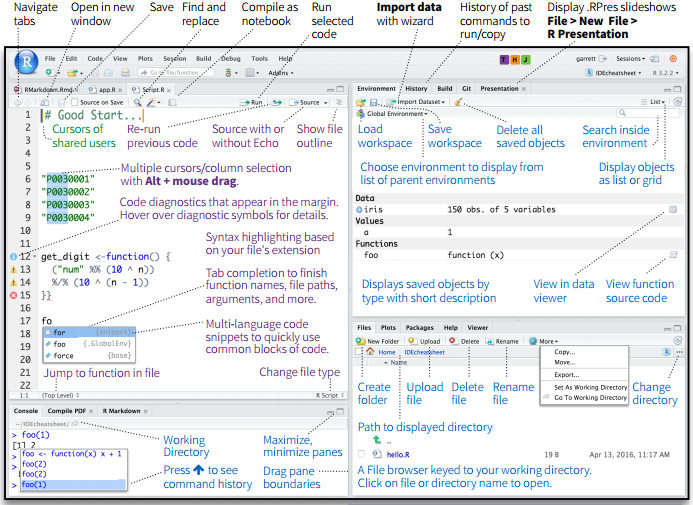
\includegraphics{figuras/rstudio_ide.png}
\caption{Fonte:
\href{https://github.com/rstudio/cheatsheets/raw/master/rstudio-ide.pdf}{RStudio
IDE Cheatsheet}}
\end{figure}

Além de poder baixar o programa utilizado nesse curso, você também pode
acessar muitos materiais como as
\href{https://www.rstudio.com/resources/cheatsheets/}{Cheatsheets} e
\href{https://www.rstudio.com/resources/webinars/}{Webnários} que cobrem
desde itens básicos como funções essenciais do RStudio até
desenvolvimento de páginas para Web ou apps com Shiny. Explore o máximo
que puder!

\textbf{Dicas:}

\begin{itemize}
\tightlist
\item
  Se não souber usar uma função, escreva: \texttt{?função}
\item
  As funções tem argumentos, use \textbf{TAB} para vê-los numa função
\end{itemize}

\section{IMPORTANTE}\label{importante}

\begin{itemize}
\tightlist
\item
  \textbf{TAB} no \textbf{RStudio}
\end{itemize}

Isso te ajudará a evitar coisas como: grafia errada da função, verificar
se a função existe, verificar argumentos, etc\ldots{} Use sempre!


\includegraphics{figuras/tab-key-.jpeg}

\begin{itemize}
\tightlist
\item
  \textbf{Stack Overflow}
  (\href{https://stackoverflow.com/questions/tagged/r}{Veja as últimas
  das mais de 240000 (!!!) perguntas sobre R})
\end{itemize}

Melhor forma de resolver problemas! Acredite, é praticamente impossível
existir um problema que outra pessoa não tenha resolvido pelo Stack
Overflow.

\begin{quote}
\emph{Eu mesma só precisei fazer \textbf{uma} pergunta no Stack Overflow
(e acabei respondendo eu mesma depois de resolver) usando R há uns 5
anos!} - Camila.
\end{quote}

\textbf{Vamos começar!}

\chapter{R!}\label{r}

A linguagem R pode ser usada desde uma simples calculadora até uma
poderosa ferramenta estatística, seja para análise de dados, seja para
machine learning.

Nesse capítulo veremos o básico da linguagem. Como a ideia é cobrir o
máximo de conteúdo possível, passaremos bem rápido pelos conceitos
básicos, com alguns exercícios para melhor entendimento.

\section{Variáveis Básicas}\label{variaveis-basicas}

Podemos armazenar valores, strings ou operadores lógicos nas chamadas
variáveis básicas. É com elas que podemos fazer operações básicas e
transformar o RStudio em uma calculadora superpoderosa. Existem 5 tipos
de variáveis básicas, sendo elas:

\begin{itemize}
\tightlist
\item
  Numeric (1): valores numéricos com ou sem casa decimal
\end{itemize}

\begin{Shaded}
\begin{Highlighting}[]
\DecValTok{5}\OperatorTok{+}\FloatTok{2.3}
\end{Highlighting}
\end{Shaded}

\begin{verbatim}
## [1] 7.3
\end{verbatim}

\begin{Shaded}
\begin{Highlighting}[]
\NormalTok{pi}
\end{Highlighting}
\end{Shaded}

\begin{verbatim}
## [1] 3.141593
\end{verbatim}

\begin{itemize}
\tightlist
\item
  \emph{Character} (a): com eles podemos armazenar strings, como o
  título de um gráfico
\end{itemize}

\begin{Shaded}
\begin{Highlighting}[]
\NormalTok{titulo <-}\StringTok{ "Isso é uma string"}
\NormalTok{titulo}
\end{Highlighting}
\end{Shaded}

\begin{verbatim}
## [1] "Isso é uma string"
\end{verbatim}

\begin{itemize}
\item
  \emph{Integer} (1): são valores inteiros
\item
  \emph{Complex} (0+1i): também é possível armazenar valores complexos
  nas variáveis básicas
\end{itemize}

\begin{Shaded}
\begin{Highlighting}[]
\DecValTok{3} \OperatorTok{+}\StringTok{ }\NormalTok{4i}
\end{Highlighting}
\end{Shaded}

\begin{verbatim}
## [1] 3+4i
\end{verbatim}

\begin{itemize}
\tightlist
\item
  \emph{Logical} (TRUE): são os famosos operadores Booleanos, que
  permitem realizar comparações entre variáveis ou dados (\textbf{Você
  não pode criar uma variável com os nomes TRUE ou FALSE, esses nomes
  são reservados pelo R})
\end{itemize}

\begin{Shaded}
\begin{Highlighting}[]
\DecValTok{1} \OperatorTok{==}\StringTok{ }\DecValTok{2}
\end{Highlighting}
\end{Shaded}

\begin{verbatim}
## [1] FALSE
\end{verbatim}

\section{Vetores}\label{vetores}

Vetores permitem que você armazene dados em uma sequência 1D de qualquer
um dos tipos listados nas variáveis básicas, mais o formato ``cru''
(raw) que é o modo de armazenamento de bytes. Por exemplo:

\begin{itemize}
\tightlist
\item
  c(``A'', ``C'', ``D'')
\item
  1:5 = c(1, 2, 3, 4, 5)
\item
  c(TRUE, FALSE)
\item
  c(1i, -1i)
\end{itemize}

\textbf{Importante: ao contrário do C ou do Python, na linguagem R, a
contagem das posições dos vetores começa do 1 e NÃO do zero!}

\section{Classe}\label{classe}

Como foi possível notar, todas as variáveis pertencem a alguma classe,
dessa forma, a função \texttt{class} permite descobrir qual a classe da
variável que se está utilizando:

\begin{Shaded}
\begin{Highlighting}[]
\NormalTok{x <-}\StringTok{ }\KeywordTok{c}\NormalTok{(}\DecValTok{1}\NormalTok{,}\DecValTok{2}\NormalTok{,}\DecValTok{3}\NormalTok{)}
\KeywordTok{class}\NormalTok{(x)}
\end{Highlighting}
\end{Shaded}

\begin{verbatim}
## [1] "numeric"
\end{verbatim}

\begin{center}\rule{0.5\linewidth}{\linethickness}\end{center}

{\textbf{Exercício}: Qual a classe dos seguintes vetores?}

\texttt{c(1,\ “C”,\ “D”)}\\
\texttt{c(1,\ NA,\ “D”)}\\
\texttt{c(1,\ NA,\ NaN)}

\begin{center}\rule{0.5\linewidth}{\linethickness}\end{center}

\section{Converter objetos}\label{converter-objetos}

Às vezes quando trabalhamos com dados, podemos precisar ``arredondar''
valores ou converter vetores em listas, para isso existem algumas
funções especiais.

\subsection{\texorpdfstring{\texttt{as}}{as}}\label{as}

Um modo de forçar um objeto a assumir outra classe é por meio da função
\texttt{as}:

\begin{Shaded}
\begin{Highlighting}[]
\KeywordTok{as.integer}\NormalTok{(}\KeywordTok{c}\NormalTok{(}\FloatTok{1.5}\NormalTok{, }\FloatTok{2.9}\NormalTok{, }\DecValTok{1}\NormalTok{))}
\end{Highlighting}
\end{Shaded}

\begin{verbatim}
## [1] 1 2 1
\end{verbatim}

Note que a função apenas converte os números de decimais para inteiros,
sem arredondar para o número mais próximo.

\begin{center}\rule{0.5\linewidth}{\linethickness}\end{center}

{\textbf{Pergunta}: O que acontece quando se tenta converter o seguinte
vetor?}

\texttt{as.numeric(c(1,\ "C",\ "D"))}

\begin{center}\rule{0.5\linewidth}{\linethickness}\end{center}

\hypertarget{convert_df}{\subsection{\texorpdfstring{\texttt{merge} e
\texttt{melt}}{merge e melt}}\label{convert_df}}

Nem sempre os conjuntos de dados que você encontrar pela vida estarão no
formato desejado para plotar e/ou analisar estatisticamente, dessa
forma, essas duas funções poderão ajudar na sua jornada:

\begin{itemize}
\tightlist
\item
  \texttt{merge}: permite a união entre dois
  \protect\hyperlink{dataframes}{data frames}, seja por colunas em comum
  ou linhas em comum
\item
  \texttt{melt}: do pacote
  \href{https://cran.r-project.org/web/packages/reshape2/reshape2.pdf}{reshape2},
  permite que você agrupe várias colunas em função de outra coluna em
  comum, de acordo com o nome especificado
\end{itemize}

\section{Array}\label{array}

Ao contrário do vetor unidimensional, arrays permietm que você armazene
dados em diversas dimensões, sendo todas com o mesmo comprimento.

Vamos dar uma olhada nos argumentos da função:

\begin{Shaded}
\begin{Highlighting}[]
\KeywordTok{args}\NormalTok{(array)}
\end{Highlighting}
\end{Shaded}

\begin{verbatim}
## function (data = NA, dim = length(data), dimnames = NULL) 
## NULL
\end{verbatim}

Dessa forma, é preciso ``informar'' ao R qual o número de dimensões que
você quer no seu array:

\begin{Shaded}
\begin{Highlighting}[]
\NormalTok{a <-}\StringTok{ }\KeywordTok{array}\NormalTok{(}\DataTypeTok{data =} \DecValTok{0}\NormalTok{, }\DataTypeTok{dim =} \KeywordTok{c}\NormalTok{(}\DecValTok{1}\NormalTok{,}\DecValTok{1}\NormalTok{))}
\KeywordTok{class}\NormalTok{(a)}
\end{Highlighting}
\end{Shaded}

\begin{verbatim}
## [1] "matrix"
\end{verbatim}

No caso acima, como só foram desiginadas duas dimensões, o array é igual
a uma matriz.

\begin{Shaded}
\begin{Highlighting}[]
\NormalTok{a <-}\StringTok{ }\KeywordTok{array}\NormalTok{(}\DataTypeTok{data =} \DecValTok{0}\NormalTok{, }\DataTypeTok{dim =} \KeywordTok{c}\NormalTok{(}\DecValTok{3}\NormalTok{,}\DecValTok{3}\NormalTok{,}\DecValTok{1}\NormalTok{))}
\KeywordTok{class}\NormalTok{(a)}
\end{Highlighting}
\end{Shaded}

\begin{verbatim}
## [1] "array"
\end{verbatim}

Como dá pra ver acima, é possível armazenar diversos elementos em um
array, como por exemplo as dimensões que utilizamos no dia-a-dia de
modelos numéricos: espaço (x,y,z) e tempo (z). Dessa forma, podemos
criar arrays a partir de vetores e armazená-los em diverssas dimensões.

\begin{Shaded}
\begin{Highlighting}[]
\NormalTok{vetor1 <-}\StringTok{ }\KeywordTok{c}\NormalTok{(}\DecValTok{1}\NormalTok{,}\DecValTok{2}\NormalTok{,}\DecValTok{3}\NormalTok{,}\DecValTok{4}\NormalTok{,}\DecValTok{5}\NormalTok{)}
\NormalTok{vetor2 <-}\StringTok{ }\KeywordTok{c}\NormalTok{(}\DecValTok{10}\NormalTok{,}\DecValTok{12}\NormalTok{,}\DecValTok{14}\NormalTok{,}\DecValTok{16}\NormalTok{,}\DecValTok{18}\NormalTok{,}\DecValTok{20}\NormalTok{,}\DecValTok{22}\NormalTok{,}\DecValTok{24}\NormalTok{)}

\NormalTok{a <-}\StringTok{ }\KeywordTok{array}\NormalTok{(}\DataTypeTok{data =} \KeywordTok{c}\NormalTok{(vetor1,vetor2), }\DataTypeTok{dim =} \KeywordTok{c}\NormalTok{(}\DecValTok{3}\NormalTok{,}\DecValTok{3}\NormalTok{,}\DecValTok{2}\NormalTok{))}
\KeywordTok{class}\NormalTok{(a)}
\end{Highlighting}
\end{Shaded}

\begin{verbatim}
## [1] "array"
\end{verbatim}

Se você quiser, também é possível nomear as colunas e linhas do seu
array:

\begin{Shaded}
\begin{Highlighting}[]
\NormalTok{colunas <-}\StringTok{ }\KeywordTok{c}\NormalTok{(}\StringTok{"col1"}\NormalTok{, }\StringTok{"col2"}\NormalTok{, }\StringTok{"col3"}\NormalTok{)}
\NormalTok{linhas <-}\StringTok{ }\KeywordTok{c}\NormalTok{(}\StringTok{"lin1"}\NormalTok{, }\StringTok{"lin2"}\NormalTok{, }\StringTok{"lin3"}\NormalTok{)}

\KeywordTok{array}\NormalTok{(}\DataTypeTok{data =} \KeywordTok{c}\NormalTok{(vetor1, vetor2), }\DataTypeTok{dim =} \KeywordTok{c}\NormalTok{(}\DecValTok{3}\NormalTok{, }\DecValTok{3}\NormalTok{, }\DecValTok{2}\NormalTok{), }\DataTypeTok{dimnames =} \KeywordTok{list}\NormalTok{(linhas, colunas))}
\end{Highlighting}
\end{Shaded}

\begin{verbatim}
## , , 1
## 
##      col1 col2 col3
## lin1    1    4   12
## lin2    2    5   14
## lin3    3   10   16
## 
## , , 2
## 
##      col1 col2 col3
## lin1   18   24    3
## lin2   20    1    4
## lin3   22    2    5
\end{verbatim}

Além disso, sempre que precisar acessar elementos do seu array é só
especificar aas dimensões como para mostrar o elemento de um vetor.

\begin{Shaded}
\begin{Highlighting}[]
\NormalTok{a[}\DecValTok{1}\NormalTok{,}\DecValTok{2}\NormalTok{,}\DecValTok{2}\NormalTok{] }\CommentTok{#(linha, coluna, matriz)}
\end{Highlighting}
\end{Shaded}

\begin{verbatim}
## [1] 24
\end{verbatim}

\begin{center}\rule{0.5\linewidth}{\linethickness}\end{center}

{\textbf{Exercício}: Crie um array com 3 dimensões, contendo três linhas
e 4 quatro colunas. Acesse o elemento da segunda linha e terceira coluna
desse array. Não esqueça de verificar a classe desse objeto!}

\begin{center}\rule{0.5\linewidth}{\linethickness}\end{center}

\section{\texorpdfstring{Matrizes e a função
\texttt{matrix}}{Matrizes e a função matrix}}\label{matrizes-e-a-funcao-matrix}

Uma matriz é um array com duas dimensões, sendo necessário informar o
número de colunas e linhas, mas não o de dimensões.

Assim como em arrays, só são permitidos elementos \textbf{da mesma
clase}!

Argumentos da função \texttt{matrix}:

\begin{Shaded}
\begin{Highlighting}[]
\KeywordTok{args}\NormalTok{(matrix)}
\end{Highlighting}
\end{Shaded}

\begin{verbatim}
## function (data = NA, nrow = 1, ncol = 1, byrow = FALSE, dimnames = NULL) 
## NULL
\end{verbatim}

Colocando dados em uma matriz:

\begin{Shaded}
\begin{Highlighting}[]
\NormalTok{m1 <-}\StringTok{ }\KeywordTok{matrix}\NormalTok{(}\DataTypeTok{data =} \DecValTok{1}\OperatorTok{:}\NormalTok{(}\DecValTok{4}\OperatorTok{*}\DecValTok{4}\NormalTok{), }\DataTypeTok{nrow =} \DecValTok{4}\NormalTok{, }\DataTypeTok{ncol =} \DecValTok{4}\NormalTok{)}
\KeywordTok{dim}\NormalTok{(m1)}
\end{Highlighting}
\end{Shaded}

\begin{verbatim}
## [1] 4 4
\end{verbatim}

Por padrão, a opção ``byrow'' é igual a \textbf{FALSE}. Quando passamos
para \textbf{TRUE}, é possível organizar os dados por linha.

\begin{Shaded}
\begin{Highlighting}[]
\NormalTok{m2 <-}\StringTok{ }\KeywordTok{matrix}\NormalTok{(}\DataTypeTok{data =} \DecValTok{1}\OperatorTok{:}\NormalTok{(}\DecValTok{4}\OperatorTok{*}\DecValTok{4}\NormalTok{), }\DataTypeTok{nrow =} \DecValTok{4}\NormalTok{, }\DataTypeTok{ncol =} \DecValTok{4}\NormalTok{, }\DataTypeTok{byrow =} \OtherTok{TRUE}\NormalTok{)}
\end{Highlighting}
\end{Shaded}

\begin{center}\rule{0.5\linewidth}{\linethickness}\end{center}

{\textbf{Exercício}: Construa uma matriz com três linhas que contenha os
números de 1 a 9.}

\begin{center}\rule{0.5\linewidth}{\linethickness}\end{center}

\section{Listas}\label{listas}

Já as listas permitem que você armazene qualquer tipo de variável
básica, independente da classe. Dessa forma, podemos colocar numa lista:
número, caracteres, argumentos lógicos, ou que você quiser:

\begin{Shaded}
\begin{Highlighting}[]
\KeywordTok{list}\NormalTok{(}\KeywordTok{list}\NormalTok{(}\KeywordTok{list}\NormalTok{(}\KeywordTok{list}\NormalTok{(}\DecValTok{1}\NormalTok{))))}
\end{Highlighting}
\end{Shaded}

\begin{verbatim}
## [[1]]
## [[1]][[1]]
## [[1]][[1]][[1]]
## [[1]][[1]][[1]][[1]]
## [1] 1
\end{verbatim}

Isso faz com que elas sejam bastante versáteis e sirvam para armazenar o
que você precisar, mas elas só podem ter uma dimensão, como uma fila. Já
os objetos armazenados dentro da lista não precisam ter a mesma
dimensão.

\begin{Shaded}
\begin{Highlighting}[]
\NormalTok{x <-}\StringTok{ }\KeywordTok{list}\NormalTok{(}\DecValTok{1}\NormalTok{, }\StringTok{"a"}\NormalTok{, }\OtherTok{TRUE}\NormalTok{, }\DecValTok{1} \OperatorTok{+}\StringTok{ }\NormalTok{4i)}
\end{Highlighting}
\end{Shaded}

\begin{center}\rule{0.5\linewidth}{\linethickness}\end{center}

{\textbf{Exercício}: Crie uma lista contendo um vetor, uma matriz e um
data frame e acesse o segundo elemento dela.}

{Para facilitar, já vamos te dar o data frame:}

\begin{Shaded}
\begin{Highlighting}[]
\NormalTok{my_df <-}\StringTok{ }\NormalTok{mtcars[}\DecValTok{1}\OperatorTok{:}\DecValTok{10}\NormalTok{,]}
\end{Highlighting}
\end{Shaded}

\begin{center}\rule{0.5\linewidth}{\linethickness}\end{center}

\hypertarget{dataframes}{\section{Data Frames}\label{dataframes}}

Os data frames são uma forma de armazenar seus dados em um formato
parecido com uma planilha de excel. Você pode pensar em um data frame
como uma matriz que armazena em cada coluna um dado diferente, ou como
uma lista onde todos os elementos tem o mesmo comprimento.

\begin{Shaded}
\begin{Highlighting}[]
\NormalTok{df <-}\StringTok{ }\KeywordTok{data.frame}\NormalTok{(}\DataTypeTok{a =} \DecValTok{1}\OperatorTok{:}\DecValTok{3}\NormalTok{)}
\KeywordTok{names}\NormalTok{(df)}
\end{Highlighting}
\end{Shaded}

\begin{verbatim}
## [1] "a"
\end{verbatim}

\begin{Shaded}
\begin{Highlighting}[]
\KeywordTok{class}\NormalTok{(df)}
\end{Highlighting}
\end{Shaded}

\begin{verbatim}
## [1] "data.frame"
\end{verbatim}

\begin{Shaded}
\begin{Highlighting}[]
\KeywordTok{mode}\NormalTok{(df)}
\end{Highlighting}
\end{Shaded}

\begin{verbatim}
## [1] "list"
\end{verbatim}

É normalmente em um data frame que você importará os seus dados e vale
saber como visualizar algumas informações básicas sobre ele direto no
seu console. Para isso, vamos pegar como exemplo o conjunto
\texttt{mtcars} da base de dados do R:

\begin{Shaded}
\begin{Highlighting}[]
\NormalTok{df <-}\StringTok{ }\NormalTok{mtcars}
\KeywordTok{head}\NormalTok{(df) }\CommentTok{#mostra as sete primeiras linhas do data frame}
\end{Highlighting}
\end{Shaded}

\begin{verbatim}
##                    mpg cyl disp  hp drat    wt  qsec vs am gear carb
## Mazda RX4         21.0   6  160 110 3.90 2.620 16.46  0  1    4    4
## Mazda RX4 Wag     21.0   6  160 110 3.90 2.875 17.02  0  1    4    4
## Datsun 710        22.8   4  108  93 3.85 2.320 18.61  1  1    4    1
## Hornet 4 Drive    21.4   6  258 110 3.08 3.215 19.44  1  0    3    1
## Hornet Sportabout 18.7   8  360 175 3.15 3.440 17.02  0  0    3    2
## Valiant           18.1   6  225 105 2.76 3.460 20.22  1  0    3    1
\end{verbatim}

Para ver as últimas linhas do data frame basta usar a função
\texttt{tail}. Já uma função muito útil é a \texttt{summary}, que
apresenta um ``resumo'' dos seus dados, como média, mediana, mínimos e
máximos para cada \textbf{coluna} do data frame.

\begin{Shaded}
\begin{Highlighting}[]
\KeywordTok{summary}\NormalTok{(df)}
\end{Highlighting}
\end{Shaded}

\begin{verbatim}
##       mpg             cyl             disp             hp       
##  Min.   :10.40   Min.   :4.000   Min.   : 71.1   Min.   : 52.0  
##  1st Qu.:15.43   1st Qu.:4.000   1st Qu.:120.8   1st Qu.: 96.5  
##  Median :19.20   Median :6.000   Median :196.3   Median :123.0  
##  Mean   :20.09   Mean   :6.188   Mean   :230.7   Mean   :146.7  
##  3rd Qu.:22.80   3rd Qu.:8.000   3rd Qu.:326.0   3rd Qu.:180.0  
##  Max.   :33.90   Max.   :8.000   Max.   :472.0   Max.   :335.0  
##       drat             wt             qsec             vs        
##  Min.   :2.760   Min.   :1.513   Min.   :14.50   Min.   :0.0000  
##  1st Qu.:3.080   1st Qu.:2.581   1st Qu.:16.89   1st Qu.:0.0000  
##  Median :3.695   Median :3.325   Median :17.71   Median :0.0000  
##  Mean   :3.597   Mean   :3.217   Mean   :17.85   Mean   :0.4375  
##  3rd Qu.:3.920   3rd Qu.:3.610   3rd Qu.:18.90   3rd Qu.:1.0000  
##  Max.   :4.930   Max.   :5.424   Max.   :22.90   Max.   :1.0000  
##        am              gear            carb      
##  Min.   :0.0000   Min.   :3.000   Min.   :1.000  
##  1st Qu.:0.0000   1st Qu.:3.000   1st Qu.:2.000  
##  Median :0.0000   Median :4.000   Median :2.000  
##  Mean   :0.4062   Mean   :3.688   Mean   :2.812  
##  3rd Qu.:1.0000   3rd Qu.:4.000   3rd Qu.:4.000  
##  Max.   :1.0000   Max.   :5.000   Max.   :8.000
\end{verbatim}

Iremos trabalhar bastante com data frames daqui pra frente, eles se
tornarão aliados muito poderosos.

\section{Tempo e Data}\label{tempo-e-data}

O R trabalha com três classe de tempo: \texttt{POSIXct},
\texttt{POSIXlt} e \texttt{Date}, sendo que \texttt{POSIXct} se refere
ao número de segundos desde o início de 1970 no modo UTC, enquanto que
\texttt{POSIXlt} armazena as datas como uma lista, contendo segundos,
minutos, horas, dias, meses, etc.

\begin{Shaded}
\begin{Highlighting}[]
\NormalTok{a <-}\StringTok{ }\KeywordTok{ISOdate}\NormalTok{(}\DataTypeTok{year =} \DecValTok{2018}\NormalTok{, }\DataTypeTok{month =} \DecValTok{4}\NormalTok{, }\DataTypeTok{day =} \DecValTok{5}\NormalTok{)}
\KeywordTok{class}\NormalTok{(a)}
\end{Highlighting}
\end{Shaded}

\begin{verbatim}
## [1] "POSIXct" "POSIXt"
\end{verbatim}

\begin{Shaded}
\begin{Highlighting}[]
\NormalTok{b <-}\StringTok{ }\KeywordTok{ISOdate}\NormalTok{(}\DataTypeTok{year =} \DecValTok{2018}\NormalTok{, }\DataTypeTok{month =} \DecValTok{4}\NormalTok{, }\DataTypeTok{day =} \DecValTok{5}\NormalTok{, }\DataTypeTok{tz =} \StringTok{"Americas/Sao_Paulo"}\NormalTok{)}
\end{Highlighting}
\end{Shaded}

\begin{verbatim}
## Warning in strptime(x, "%Y-%m-%d-%H-%M-%OS", tz = tz): unknown timezone
## 'Americas/Sao_Paulo'
\end{verbatim}

\begin{verbatim}
## Warning in as.POSIXct.POSIXlt(strptime(x, "%Y-%m-%d-%H-%M-%OS", tz = tz), :
## unknown timezone 'Americas/Sao_Paulo'
\end{verbatim}

Já a classe \texttt{Date}, armazena as datas como o número de dias
contados a partir de 1970.

\begin{Shaded}
\begin{Highlighting}[]
\NormalTok{c <-}\StringTok{ }\KeywordTok{as.Date}\NormalTok{(}\KeywordTok{Sys.time}\NormalTok{())}
\KeywordTok{class}\NormalTok{(c)}
\end{Highlighting}
\end{Shaded}

\begin{verbatim}
## [1] "Date"
\end{verbatim}

Caso você precise, o pacote
\href{https://github.com/eddelbuettel/nanotime}{nanotime} permite
trabalhar com nano segundos.

Também é possível fazer sequências:

\begin{Shaded}
\begin{Highlighting}[]
\NormalTok{hoje <-}\StringTok{ }\KeywordTok{Sys.time}\NormalTok{()}
\NormalTok{a <-}\StringTok{ }\KeywordTok{seq.POSIXt}\NormalTok{(}\DataTypeTok{from =}\NormalTok{ hoje, }\DataTypeTok{by =} \DecValTok{3600}\NormalTok{, }\DataTypeTok{length.out =} \DecValTok{24}\NormalTok{)}
\end{Highlighting}
\end{Shaded}

Funções úteis: \texttt{weekdays}, \texttt{month} e
\href{https://en.wikipedia.org/wiki/Julian_day}{\texttt{julian}}

\begin{Shaded}
\begin{Highlighting}[]
\KeywordTok{weekdays}\NormalTok{(a)}
\end{Highlighting}
\end{Shaded}

\begin{verbatim}
##  [1] "terça-feira"  "terça-feira"  "terça-feira"  "terça-feira" 
##  [5] "terça-feira"  "terça-feira"  "terça-feira"  "terça-feira" 
##  [9] "terça-feira"  "terça-feira"  "terça-feira"  "terça-feira" 
## [13] "terça-feira"  "quarta-feira" "quarta-feira" "quarta-feira"
## [17] "quarta-feira" "quarta-feira" "quarta-feira" "quarta-feira"
## [21] "quarta-feira" "quarta-feira" "quarta-feira" "quarta-feira"
\end{verbatim}

\begin{Shaded}
\begin{Highlighting}[]
\KeywordTok{months}\NormalTok{(a)}
\end{Highlighting}
\end{Shaded}

\begin{verbatim}
##  [1] "junho" "junho" "junho" "junho" "junho" "junho" "junho" "junho"
##  [9] "junho" "junho" "junho" "junho" "junho" "junho" "junho" "junho"
## [17] "junho" "junho" "junho" "junho" "junho" "junho" "junho" "junho"
\end{verbatim}

\begin{Shaded}
\begin{Highlighting}[]
\KeywordTok{julian}\NormalTok{(a) }\CommentTok{#dia Juliano}
\end{Highlighting}
\end{Shaded}

\begin{verbatim}
## Time differences in days
##  [1] 17687.62 17687.66 17687.70 17687.74 17687.78 17687.83 17687.87
##  [8] 17687.91 17687.95 17687.99 17688.03 17688.08 17688.12 17688.16
## [15] 17688.20 17688.24 17688.28 17688.33 17688.37 17688.41 17688.45
## [22] 17688.49 17688.53 17688.58
## attr(,"origin")
## [1] "1970-01-01 GMT"
\end{verbatim}

O formato \texttt{POSIXct} é o mais comumente usado principalmente se os
dados analisados serão plotados.

\section{Fatores}\label{fatores}

Os \texttt{factors} podem ser um pouco infernais. Dê uma olhada em
\href{http://www.burns-stat.com/documents/books/the-r-inferno/}{R
INFERNO}.\\
Usados em análise estatísica, fatores são usados para armazenar
variáveis categóricas, ou seja, é uma variável que pode pertencer a um
número limitado de categorias, como por exemplo, dias da semana. Já uma
variável contínua pode assumir um um número infinito de valores.

\begin{Shaded}
\begin{Highlighting}[]
\NormalTok{a <-}\StringTok{ }\KeywordTok{seq.POSIXt}\NormalTok{(}\DataTypeTok{from =}\NormalTok{ hoje , }\DataTypeTok{by =} \DecValTok{3600}\NormalTok{, }\DataTypeTok{length.out =} \DecValTok{24}\OperatorTok{*}\DecValTok{7}\NormalTok{)}
\NormalTok{aa <-}\StringTok{ }\KeywordTok{weekdays}\NormalTok{(a)}
\KeywordTok{class}\NormalTok{(aa)}
\end{Highlighting}
\end{Shaded}

\begin{verbatim}
## [1] "character"
\end{verbatim}

\begin{Shaded}
\begin{Highlighting}[]
\KeywordTok{factor}\NormalTok{(aa)}
\end{Highlighting}
\end{Shaded}

\begin{verbatim}
##   [1] terça-feira   terça-feira   terça-feira   terça-feira   terça-feira  
##   [6] terça-feira   terça-feira   terça-feira   terça-feira   terça-feira  
##  [11] terça-feira   terça-feira   terça-feira   quarta-feira  quarta-feira 
##  [16] quarta-feira  quarta-feira  quarta-feira  quarta-feira  quarta-feira 
##  [21] quarta-feira  quarta-feira  quarta-feira  quarta-feira  quarta-feira 
##  [26] quarta-feira  quarta-feira  quarta-feira  quarta-feira  quarta-feira 
##  [31] quarta-feira  quarta-feira  quarta-feira  quarta-feira  quarta-feira 
##  [36] quarta-feira  quarta-feira  quinta-feira  quinta-feira  quinta-feira 
##  [41] quinta-feira  quinta-feira  quinta-feira  quinta-feira  quinta-feira 
##  [46] quinta-feira  quinta-feira  quinta-feira  quinta-feira  quinta-feira 
##  [51] quinta-feira  quinta-feira  quinta-feira  quinta-feira  quinta-feira 
##  [56] quinta-feira  quinta-feira  quinta-feira  quinta-feira  quinta-feira 
##  [61] quinta-feira  sexta-feira   sexta-feira   sexta-feira   sexta-feira  
##  [66] sexta-feira   sexta-feira   sexta-feira   sexta-feira   sexta-feira  
##  [71] sexta-feira   sexta-feira   sexta-feira   sexta-feira   sexta-feira  
##  [76] sexta-feira   sexta-feira   sexta-feira   sexta-feira   sexta-feira  
##  [81] sexta-feira   sexta-feira   sexta-feira   sexta-feira   sexta-feira  
##  [86] sábado        sábado        sábado        sábado        sábado       
##  [91] sábado        sábado        sábado        sábado        sábado       
##  [96] sábado        sábado        sábado        sábado        sábado       
## [101] sábado        sábado        sábado        sábado        sábado       
## [106] sábado        sábado        sábado        sábado        domingo      
## [111] domingo       domingo       domingo       domingo       domingo      
## [116] domingo       domingo       domingo       domingo       domingo      
## [121] domingo       domingo       domingo       domingo       domingo      
## [126] domingo       domingo       domingo       domingo       domingo      
## [131] domingo       domingo       domingo       segunda-feira segunda-feira
## [136] segunda-feira segunda-feira segunda-feira segunda-feira segunda-feira
## [141] segunda-feira segunda-feira segunda-feira segunda-feira segunda-feira
## [146] segunda-feira segunda-feira segunda-feira segunda-feira segunda-feira
## [151] segunda-feira segunda-feira segunda-feira segunda-feira segunda-feira
## [156] segunda-feira segunda-feira terça-feira   terça-feira   terça-feira  
## [161] terça-feira   terça-feira   terça-feira   terça-feira   terça-feira  
## [166] terça-feira   terça-feira   terça-feira  
## 7 Levels: domingo quarta-feira quinta-feira sábado ... terça-feira
\end{verbatim}

São muito úteis para regressões, gráficos e resumos estatísitcos, uma
vez que limita o número de possibilidades para a qual o dado pertença.
Além disso, é possível estabelecer ``níveis'' que vão designar a
categoria do seu dado.

\begin{Shaded}
\begin{Highlighting}[]
\NormalTok{ab <-}\StringTok{ }\KeywordTok{factor}\NormalTok{(}\DataTypeTok{x =}\NormalTok{ aa,}
             \DataTypeTok{levels =} \KeywordTok{c}\NormalTok{(}\StringTok{"Monday"}\NormalTok{, }\StringTok{"Tuesday"}\NormalTok{,  }\StringTok{"Wednesday"}\NormalTok{,  }\StringTok{"Thursday"}\NormalTok{,}
                        \StringTok{"Friday"}\NormalTok{, }\StringTok{"Saturday"}\NormalTok{, }\StringTok{"Sunday"}\NormalTok{))}
\KeywordTok{levels}\NormalTok{(ab)}
\end{Highlighting}
\end{Shaded}

\begin{verbatim}
## [1] "Monday"    "Tuesday"   "Wednesday" "Thursday"  "Friday"    "Saturday" 
## [7] "Sunday"
\end{verbatim}

\begin{center}\rule{0.5\linewidth}{\linethickness}\end{center}

{\textbf{Exercício}: Converta o vetor abaixo em um fator e mostre os
seus níveis}

\texttt{genero\ \textless{}-\ c("Masculino",\ "Masculino",\ "Feminino",\ "Masculino",\ "Feminino",\ "Feminino")}

\begin{center}\rule{0.5\linewidth}{\linethickness}\end{center}

Se tudo pareceu muito corrido, não se preocupe, todos esses conceitos
serão praticados mais adiante!

\begin{Shaded}
\begin{Highlighting}[]
\CommentTok{#-- Opção para deixar possível visualizar erros}
\NormalTok{knitr}\OperatorTok{::}\NormalTok{opts_chunk}\OperatorTok{$}\KeywordTok{set}\NormalTok{(}\DataTypeTok{error =} \OtherTok{TRUE}\NormalTok{)}
\end{Highlighting}
\end{Shaded}

\chapter{Importando e Exportando
Dados}\label{importando-e-exportando-dados}

\section{Base}\label{base}

\subsection{\texorpdfstring{Importando com
\texttt{read.*}}{Importando com read.*}}\label{importando-com-read.}

Como vimos anteriormente, na maioria dos casos, iremos usar data frames
par lidar com dados em R, sendo assim, podemos utilizar os seguintes
modos de leitura:

\begin{itemize}
\tightlist
\item
  \texttt{read.csv}\\
\item
  \texttt{read.csv2}\\
\item
  \texttt{read.table}
\end{itemize}

Vamos ler alguns dados usando \texttt{read.table}. Para saber o que a
função faz, use \texttt{?read.table}.\\
Os argumentos da função são:

\begin{Shaded}
\begin{Highlighting}[]
\KeywordTok{args}\NormalTok{(read.table)}
\end{Highlighting}
\end{Shaded}

\begin{verbatim}
## function (file, header = FALSE, sep = "", quote = "\"'", dec = ".", 
##     numerals = c("allow.loss", "warn.loss", "no.loss"), row.names, 
##     col.names, as.is = !stringsAsFactors, na.strings = "NA", 
##     colClasses = NA, nrows = -1, skip = 0, check.names = TRUE, 
##     fill = !blank.lines.skip, strip.white = FALSE, blank.lines.skip = TRUE, 
##     comment.char = "#", allowEscapes = FALSE, flush = FALSE, 
##     stringsAsFactors = default.stringsAsFactors(), fileEncoding = "", 
##     encoding = "unknown", text, skipNul = FALSE) 
## NULL
\end{verbatim}

O terceiro argumento é \texttt{sep}, definido como \texttt{""} por
padrão. Esse argumento indica para o R qual o tipo de separador
utilizado entre as colunas dos dados.

\begin{Shaded}
\begin{Highlighting}[]
\NormalTok{df <-}\StringTok{ }\KeywordTok{read.table}\NormalTok{(}\StringTok{"dados/NOXIPEN2014.txt"}\NormalTok{)}
\end{Highlighting}
\end{Shaded}

Lembre-se que as funções \texttt{head} e \texttt{tail} permitem que você
veja as primeiras ou últimas linhas do data frame.

\begin{Shaded}
\begin{Highlighting}[]
\KeywordTok{head}\NormalTok{(df)}
\end{Highlighting}
\end{Shaded}

\begin{verbatim}
##    TipodeRede TipodeMonitoramento             Tipo       Data  Hora
## 2 Automático              CETESB Dados Primários 01/01/2014 01:00
## 3 Automático              CETESB Dados Primários 01/01/2014 02:00
## 4 Automático              CETESB Dados Primários 01/01/2014 03:00
## 5 Automático              CETESB Dados Primários 01/01/2014 04:00
## 6 Automático              CETESB Dados Primários 01/01/2014 05:00
## 7 Automático              CETESB Dados Primários 01/01/2014 06:00
##   CodigoEstaÃ.Ã.o               NomeEstaÃ.Ã.o               NomeParÃ.metro
## 2              95 Cid.Universitária-USP-Ipen NOx (Óxidos de Nitrogênio)
## 3              95 Cid.Universitária-USP-Ipen NOx (Óxidos de Nitrogênio)
## 4              95 Cid.Universitária-USP-Ipen NOx (Óxidos de Nitrogênio)
## 5              95 Cid.Universitária-USP-Ipen NOx (Óxidos de Nitrogênio)
## 6              95 Cid.Universitária-USP-Ipen NOx (Óxidos de Nitrogênio)
## 7              95 Cid.Universitária-USP-Ipen NOx (Óxidos de Nitrogênio)
##   UnidadedeMedida MediaHoraria MediaMovel Valido
## 2             ppb            9          -   Não
## 3             ppb            9          -    Sim
## 4             ppb            5          -    Sim
## 5             ppb            4          -    Sim
## 6             ppb            5          -    Sim
## 7             ppb            5          -    Sim
\end{verbatim}

\begin{Shaded}
\begin{Highlighting}[]
\KeywordTok{tail}\NormalTok{(df)}
\end{Highlighting}
\end{Shaded}

\begin{verbatim}
##       TipodeRede TipodeMonitoramento             Tipo       Data  Hora
## 8577 Automático              CETESB Dados Primários 01/01/2015 19:00
## 8578 Automático              CETESB Dados Primários 01/01/2015 20:00
## 8579 Automático              CETESB Dados Primários 01/01/2015 21:00
## 8580 Automático              CETESB Dados Primários 01/01/2015 22:00
## 8581 Automático              CETESB Dados Primários 01/01/2015 23:00
## 8582 Automático              CETESB Dados Primários 01/01/2015 24:00
##      CodigoEstaÃ.Ã.o               NomeEstaÃ.Ã.o
## 8577              95 Cid.Universitária-USP-Ipen
## 8578              95 Cid.Universitária-USP-Ipen
## 8579              95 Cid.Universitária-USP-Ipen
## 8580              95 Cid.Universitária-USP-Ipen
## 8581              95 Cid.Universitária-USP-Ipen
## 8582              95 Cid.Universitária-USP-Ipen
##                    NomeParÃ.metro UnidadedeMedida MediaHoraria MediaMovel
## 8577 NOx (Óxidos de Nitrogênio)             ppb            3          -
## 8578 NOx (Óxidos de Nitrogênio)             ppb            8          -
## 8579 NOx (Óxidos de Nitrogênio)             ppb           11          -
## 8580 NOx (Óxidos de Nitrogênio)             ppb           11          -
## 8581 NOx (Óxidos de Nitrogênio)             ppb           16          -
## 8582 NOx (Óxidos de Nitrogênio)             ppb           NA          -
##      Valido
## 8577    Sim
## 8578    Sim
## 8579    Sim
## 8580    Sim
## 8581    Sim
## 8582    Sim
\end{verbatim}

Vamos tentar ler outra versão dos mesmos dados utilizando a mesma função
\texttt{read.table}:

\begin{Shaded}
\begin{Highlighting}[]
\NormalTok{df2 <-}\StringTok{ }\KeywordTok{read.table}\NormalTok{(}\StringTok{"dados/NOXIPEN2014v2.txt"}\NormalTok{)}
\end{Highlighting}
\end{Shaded}

\begin{verbatim}
## Error in scan(file = file, what = what, sep = sep, quote = quote, dec = dec, : linha 1 não tinha 6 elementos
\end{verbatim}

Apareceu uma mensagem de erro, {você saberia dizer o porquê?}

\textbf{Caso você trabalhe com algum banco de dados em formato .txt e
quiser abrir no R\ldots{} Abra-os no bloco de notas primeiro!}

Vamos dar uma olhada em alguns dados, o primeiro tem uma cara assim:

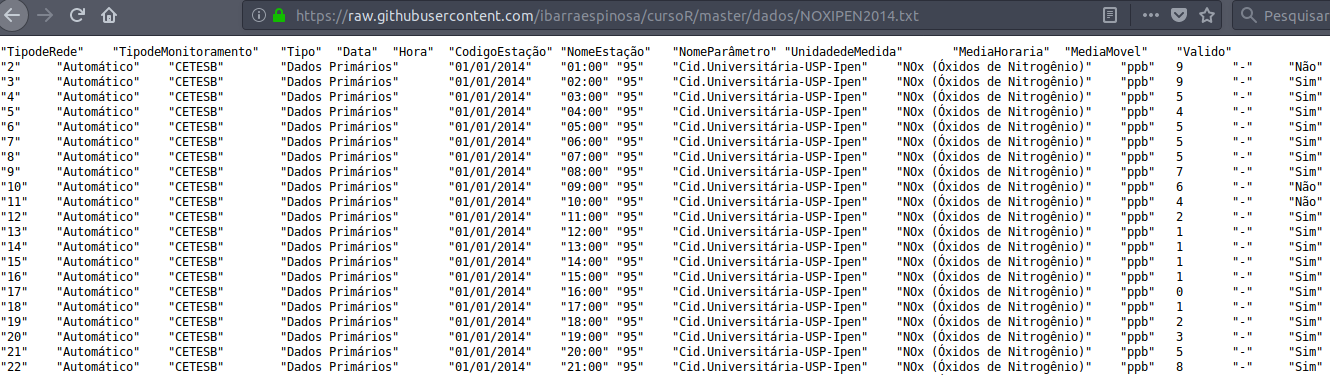
\includegraphics[width=18.47in]{figuras/f1}

Já o segundo arquivo é assim:

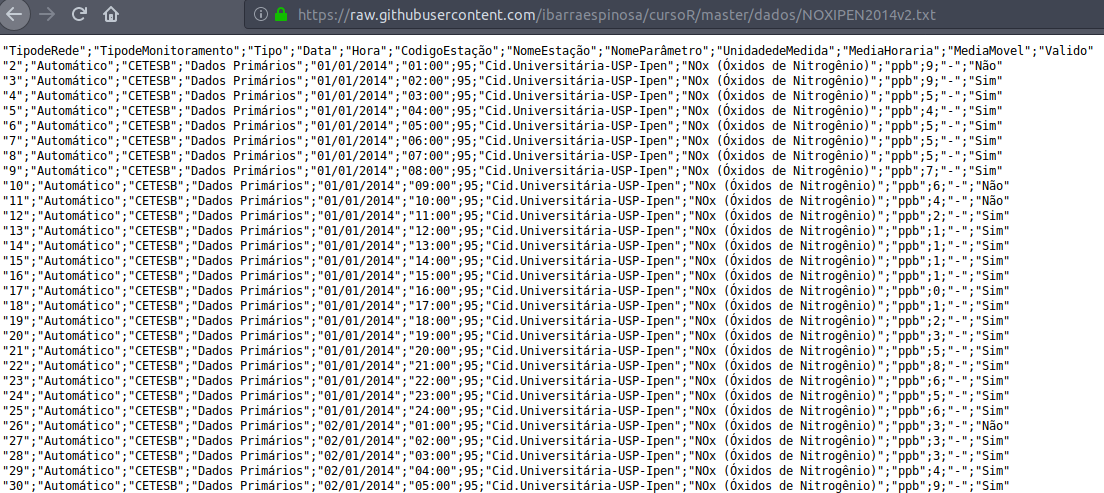
\includegraphics[width=15.33in]{figuras/f2}

Você notou a diferença? Como vimos anteriormente, para importar os dados
no R é super importante que você especifique o tipo de separador
utilizado. Como o segundo arquivo é separado por ``;'', precisamos
espercificar o argumento \texttt{sep} na hora de usar o comando
\texttt{read.table}:

\begin{Shaded}
\begin{Highlighting}[]
\NormalTok{df2 <-}\StringTok{ }\KeywordTok{read.table}\NormalTok{(}\StringTok{"dados/NOXIPEN2014v2.txt"}\NormalTok{, }\DataTypeTok{sep =} \StringTok{";"}\NormalTok{)}
\KeywordTok{head}\NormalTok{(df2)}
\end{Highlighting}
\end{Shaded}

\begin{verbatim}
##    TipodeRede TipodeMonitoramento             Tipo       Data  Hora
## 2 Automático              CETESB Dados Primários 01/01/2014 01:00
## 3 Automático              CETESB Dados Primários 01/01/2014 02:00
## 4 Automático              CETESB Dados Primários 01/01/2014 03:00
## 5 Automático              CETESB Dados Primários 01/01/2014 04:00
## 6 Automático              CETESB Dados Primários 01/01/2014 05:00
## 7 Automático              CETESB Dados Primários 01/01/2014 06:00
##   CodigoEstaÃ.Ã.o               NomeEstaÃ.Ã.o               NomeParÃ.metro
## 2              95 Cid.Universitária-USP-Ipen NOx (Óxidos de Nitrogênio)
## 3              95 Cid.Universitária-USP-Ipen NOx (Óxidos de Nitrogênio)
## 4              95 Cid.Universitária-USP-Ipen NOx (Óxidos de Nitrogênio)
## 5              95 Cid.Universitária-USP-Ipen NOx (Óxidos de Nitrogênio)
## 6              95 Cid.Universitária-USP-Ipen NOx (Óxidos de Nitrogênio)
## 7              95 Cid.Universitária-USP-Ipen NOx (Óxidos de Nitrogênio)
##   UnidadedeMedida MediaHoraria MediaMovel Valido
## 2             ppb            9          -   Não
## 3             ppb            9          -    Sim
## 4             ppb            5          -    Sim
## 5             ppb            4          -    Sim
## 6             ppb            5          -    Sim
## 7             ppb            5          -    Sim
\end{verbatim}

\begin{Shaded}
\begin{Highlighting}[]
\KeywordTok{tail}\NormalTok{(df2)}
\end{Highlighting}
\end{Shaded}

\begin{verbatim}
##       TipodeRede TipodeMonitoramento             Tipo       Data  Hora
## 8577 Automático              CETESB Dados Primários 01/01/2015 19:00
## 8578 Automático              CETESB Dados Primários 01/01/2015 20:00
## 8579 Automático              CETESB Dados Primários 01/01/2015 21:00
## 8580 Automático              CETESB Dados Primários 01/01/2015 22:00
## 8581 Automático              CETESB Dados Primários 01/01/2015 23:00
## 8582 Automático              CETESB Dados Primários 01/01/2015 24:00
##      CodigoEstaÃ.Ã.o               NomeEstaÃ.Ã.o
## 8577              95 Cid.Universitária-USP-Ipen
## 8578              95 Cid.Universitária-USP-Ipen
## 8579              95 Cid.Universitária-USP-Ipen
## 8580              95 Cid.Universitária-USP-Ipen
## 8581              95 Cid.Universitária-USP-Ipen
## 8582              95 Cid.Universitária-USP-Ipen
##                    NomeParÃ.metro UnidadedeMedida MediaHoraria MediaMovel
## 8577 NOx (Óxidos de Nitrogênio)             ppb            3          -
## 8578 NOx (Óxidos de Nitrogênio)             ppb            8          -
## 8579 NOx (Óxidos de Nitrogênio)             ppb           11          -
## 8580 NOx (Óxidos de Nitrogênio)             ppb           11          -
## 8581 NOx (Óxidos de Nitrogênio)             ppb           16          -
## 8582 NOx (Óxidos de Nitrogênio)             ppb           NA          -
##      Valido
## 8577    Sim
## 8578    Sim
## 8579    Sim
## 8580    Sim
## 8581    Sim
## 8582    Sim
\end{verbatim}

Além desses comandos, vocês também pode utilizar a opção \textbf{Import
Dataset} do RStudio, permitindo que você tenha um ``preview'' dos dados
- como no Excel, mas melhor!

Para mais informações sobre importar dados no R, dê uma olha nesse
\href{https://www.rstudio.com/resources/webinars/importing-data-into-r/}{webnário}.

\subsection{\texorpdfstring{Exportando com
\texttt{write.table}}{Exportando com write.table}}\label{exportando-com-write.table}

Exportar é bem facil. Vamos dar uma olhada nos argumentos da função
\texttt{write.table}:

\begin{Shaded}
\begin{Highlighting}[]
\KeywordTok{args}\NormalTok{(write.table)}
\end{Highlighting}
\end{Shaded}

\begin{verbatim}
## function (x, file = "", append = FALSE, quote = TRUE, sep = " ", 
##     eol = "\n", na = "NA", dec = ".", row.names = TRUE, col.names = TRUE, 
##     qmethod = c("escape", "double"), fileEncoding = "") 
## NULL
\end{verbatim}

Se temos um data frame com colunas de classe character,
\texttt{quote\ =\ TRUE} quer dizer que o arquivo de texto resultante vai
ter aspas nas colunas de caractere. Novamente, o argumento \texttt{sep}
indica como podemos separar as colunas. Se você quiser abrir esses dados
no excel, uma boa opção é utilizar os separadores ``,''/``;''/"
``/''\t``, sendo o último o separador que indica o espaçamento criado
pela tecla TAB.

Já o argumento \texttt{eol} quer dizer \emph{end of line}, e é uma forma
de dizer ao R que a linha acaba ali. Por padrão, a opção
\texttt{row.names} vem com a opção TRUE, mas sempre coloque a opção
FALSE, caso contrário, será adicionada uma coluna com os índices das
linhas. O argumento \texttt{col.names} indica se você quer nomear as
suas colunas, o que é sempre uma boa ideia.

\begin{center}\rule{0.5\linewidth}{\linethickness}\end{center}

\textbf{Exercício}: Usando o conjunto de dados \texttt{mtcars} da base
do R, exporte-o de uma forma que ele possa ser lido em algum Excel
genérico. Não esqueça de usar o que foi ensinado acima.

\begin{center}\rule{0.5\linewidth}{\linethickness}\end{center}

\subsection{\texorpdfstring{Exportando objetos com
\texttt{save}}{Exportando objetos com save}}\label{exportando-objetos-com-save}

Podemos salvar objetos do R com o comando \texttt{save}. Ele permite que
você recarregue o objeto mais tarde.

\begin{Shaded}
\begin{Highlighting}[]
\KeywordTok{args}\NormalTok{(save)}
\end{Highlighting}
\end{Shaded}

\begin{verbatim}
## function (..., list = character(), file = stop("'file' must be specified"), 
##     ascii = FALSE, version = NULL, envir = parent.frame(), compress = isTRUE(!ascii), 
##     compression_level, eval.promises = TRUE, precheck = TRUE) 
## NULL
\end{verbatim}

Essa função salva o objeto com a extensão .rda sendo que para carregá-lo
de volta usamos a função \texttt{load}

\begin{Shaded}
\begin{Highlighting}[]
\KeywordTok{args}\NormalTok{(load)}
\end{Highlighting}
\end{Shaded}

\begin{verbatim}
## function (file, envir = parent.frame(), verbose = FALSE) 
## NULL
\end{verbatim}

Muito cuidado ao utilizar esse comando, pois é bem possível cometer
alguns deslizes, como trocar o nome do objeto. Veja esse exemplo abaixo:

\begin{Shaded}
\begin{Highlighting}[]
\CommentTok{#Primeiro vamos ler os dados do dia 01/06/2016 para uma estação automática do INMET de Paracatu:}
\NormalTok{paracatu <-}\StringTok{ }\KeywordTok{read.csv}\NormalTok{(}\DataTypeTok{file =} \StringTok{"dados/paracatu.csv"}\NormalTok{, }\DataTypeTok{sep =} \StringTok{","}\NormalTok{) }\CommentTok{#lendo como csv}

\CommentTok{# Vamos dizer que queremos salvar apenas a coluna correspondente à temperatura máxima horária:}
\NormalTok{paracatu_temp <-}\StringTok{ }\NormalTok{paracatu}\OperatorTok{$}\NormalTok{temp_max  }

\CommentTok{#Agora vamos salvar o objeto do tipo numeric com o nome especificado:}
\KeywordTok{save}\NormalTok{(paracatu_temp, }\DataTypeTok{file =} \StringTok{"Temp_max.rda"}\NormalTok{)}
\end{Highlighting}
\end{Shaded}

Passado um tempo, queremos acessar de volta esse objeto, mas não
lembramos se salvamos a temperatura máxima ou mínima, vamos confiar que
foi a mínima:

\begin{Shaded}
\begin{Highlighting}[]
\KeywordTok{load}\NormalTok{(}\StringTok{"Temp_min.rda"}\NormalTok{)}
\end{Highlighting}
\end{Shaded}

E assim descobrimos que não era\ldots{} O que nos ensina a sempre
guardar na memória quais variáveis que salvamos no ambiente R. O bom
dessa função é que ela permite salvar com tipos de compressão, por
exemplo \texttt{compress\ =\ "xz"}.

\subsection{\texorpdfstring{Exportando objetos com
\texttt{saveRDS}}{Exportando objetos com saveRDS}}\label{exportando-objetos-com-saverds}

Esta é uma das minhas funçoes favoritas no R, veja só o porquê:

\begin{Shaded}
\begin{Highlighting}[]
\KeywordTok{saveRDS}\NormalTok{(paracatu_temp, }\StringTok{"Temperatura.rds"}\NormalTok{)}
\end{Highlighting}
\end{Shaded}

\begin{Shaded}
\begin{Highlighting}[]
\NormalTok{frenteQ <-}\StringTok{ }\KeywordTok{readRDS}\NormalTok{(}\StringTok{"Temperatura.rds"}\NormalTok{)}
\end{Highlighting}
\end{Shaded}

Você pode salvar seu objeto R de forma serializada e compactada com o
argumento \texttt{compress} e na hora de chamar o objeto de volta é só
usar \texttt{readRDS} e colocar o nome que você quiser.

\hypertarget{processing_dfs}{\subsection{Processando nossa data
frame}\label{processing_dfs}}

Vamos revisar a classe de cada coluna do nosso data-frame com a função
\texttt{sapply}, que será explicada em outro capítulo. Lembre-se,
qualquer dúvida é só usar \texttt{?sapply}.

\begin{Shaded}
\begin{Highlighting}[]
\KeywordTok{sapply}\NormalTok{(df, class)}
\end{Highlighting}
\end{Shaded}

\begin{verbatim}
##          TipodeRede TipodeMonitoramento                Tipo 
##            "factor"            "factor"            "factor" 
##                Data                Hora     CodigoEstaÃ.Ã.o 
##            "factor"            "factor"           "integer" 
##       NomeEstaÃ.Ã.o      NomeParÃ.metro     UnidadedeMedida 
##            "factor"            "factor"            "factor" 
##        MediaHoraria          MediaMovel              Valido 
##           "integer"            "factor"            "factor"
\end{verbatim}

Quando trabalhamos com séries temporais, é importante ter a variável
tempo reconhecida como ``tempo'', especificamente como classe
``POSIXct''. Porém, a classe do tipo Data é ``factor'' assim como a
Hora, o que pode ser ruim. Então, vamos criar uma variável de tempo mais
padronizada com o formato 2018-06-05 11:49:27.

Para isso temos que juntar as variáveis Data e Hora. Faremos isso numa
nova varável chamada ``tempo\_char'', adicionando-a diretamente no data
frame com o cifrão (``\$''). Podemos fazer isso com as funções
\texttt{paste} ou \texttt{paste0}.

\begin{Shaded}
\begin{Highlighting}[]
\NormalTok{df}\OperatorTok{$}\NormalTok{tempo_char <-}\StringTok{ }\KeywordTok{paste}\NormalTok{(df}\OperatorTok{$}\NormalTok{Data, df}\OperatorTok{$}\NormalTok{Hora)}
\KeywordTok{head}\NormalTok{(df}\OperatorTok{$}\NormalTok{tempo_char)}
\end{Highlighting}
\end{Shaded}

\begin{verbatim}
## [1] "01/01/2014 01:00" "01/01/2014 02:00" "01/01/2014 03:00"
## [4] "01/01/2014 04:00" "01/01/2014 05:00" "01/01/2014 06:00"
\end{verbatim}

\begin{Shaded}
\begin{Highlighting}[]
\KeywordTok{class}\NormalTok{(df}\OperatorTok{$}\NormalTok{tempo_char)}
\end{Highlighting}
\end{Shaded}

\begin{verbatim}
## [1] "character"
\end{verbatim}

Melhorou, mas ainda tem clase character.

Para converter a nossa classe para POSIXct podemos usar a função
\texttt{as.POSIXct} (olhe\\
\texttt{?as.POSIXct}). Seus argumentos são:

\begin{Shaded}
\begin{Highlighting}[]
\KeywordTok{args}\NormalTok{(as.POSIXct)}
\end{Highlighting}
\end{Shaded}

\begin{verbatim}
## function (x, tz = "", ...) 
## NULL
\end{verbatim}

Então, vamos criar outra variável tempo com o formato POSIXct:

\begin{Shaded}
\begin{Highlighting}[]
\NormalTok{df}\OperatorTok{$}\NormalTok{tempo <-}\StringTok{ }\KeywordTok{as.POSIXct}\NormalTok{(}\DataTypeTok{x =}\NormalTok{ df}\OperatorTok{$}\NormalTok{tempo_char, }\DataTypeTok{tz =} \StringTok{"Americas/Sao_Paulo"}\NormalTok{, }
                       \DataTypeTok{format =} \StringTok{"%d/%m/%Y %H:%M"}\NormalTok{)}
\end{Highlighting}
\end{Shaded}

\begin{verbatim}
## Warning in strptime(x, format, tz = tz): unknown timezone 'Americas/
## Sao_Paulo'
\end{verbatim}

\begin{verbatim}
## Warning in as.POSIXct.POSIXlt(as.POSIXlt(x, tz, ...), tz, ...): unknown
## timezone 'Americas/Sao_Paulo'
\end{verbatim}

\begin{Shaded}
\begin{Highlighting}[]
\KeywordTok{head}\NormalTok{(df}\OperatorTok{$}\NormalTok{tempo)}
\end{Highlighting}
\end{Shaded}

\begin{verbatim}
## Warning in as.POSIXlt.POSIXct(x, tz): unknown timezone 'Americas/Sao_Paulo'
\end{verbatim}

\begin{verbatim}
## [1] "2014-01-01 01:00:00 GMT" "2014-01-01 02:00:00 GMT"
## [3] "2014-01-01 03:00:00 GMT" "2014-01-01 04:00:00 GMT"
## [5] "2014-01-01 05:00:00 GMT" "2014-01-01 06:00:00 GMT"
\end{verbatim}

\begin{Shaded}
\begin{Highlighting}[]
\KeywordTok{class}\NormalTok{(df}\OperatorTok{$}\NormalTok{tempo)}
\end{Highlighting}
\end{Shaded}

\begin{verbatim}
## [1] "POSIXct" "POSIXt"
\end{verbatim}

Agora, vamos extrair os dias da semana do tempo, mes e dia juliano:

\begin{Shaded}
\begin{Highlighting}[]
\NormalTok{df}\OperatorTok{$}\NormalTok{weekdays <-}\StringTok{ }\KeywordTok{format}\NormalTok{(df}\OperatorTok{$}\NormalTok{tempo, }\StringTok{"%A"}\NormalTok{)}
\end{Highlighting}
\end{Shaded}

\begin{verbatim}
## Warning in as.POSIXlt.POSIXct(x, tz): unknown timezone 'Americas/Sao_Paulo'
\end{verbatim}

\begin{Shaded}
\begin{Highlighting}[]
\KeywordTok{head}\NormalTok{(df}\OperatorTok{$}\NormalTok{weekdays)}
\end{Highlighting}
\end{Shaded}

\begin{verbatim}
## [1] "quarta-feira" "quarta-feira" "quarta-feira" "quarta-feira"
## [5] "quarta-feira" "quarta-feira"
\end{verbatim}

\begin{Shaded}
\begin{Highlighting}[]
\NormalTok{df}\OperatorTok{$}\NormalTok{mes <-}\StringTok{ }\KeywordTok{format}\NormalTok{(df}\OperatorTok{$}\NormalTok{tempo, }\StringTok{"%B"}\NormalTok{)}
\end{Highlighting}
\end{Shaded}

\begin{verbatim}
## Warning in as.POSIXlt.POSIXct(x, tz): unknown timezone 'Americas/Sao_Paulo'
\end{verbatim}

\begin{Shaded}
\begin{Highlighting}[]
\KeywordTok{head}\NormalTok{(df}\OperatorTok{$}\NormalTok{mes)}
\end{Highlighting}
\end{Shaded}

\begin{verbatim}
## [1] "janeiro" "janeiro" "janeiro" "janeiro" "janeiro" "janeiro"
\end{verbatim}

\begin{Shaded}
\begin{Highlighting}[]
\NormalTok{df}\OperatorTok{$}\NormalTok{diajuliano <-}\StringTok{ }\KeywordTok{julian}\NormalTok{(df}\OperatorTok{$}\NormalTok{tempo)}
\KeywordTok{head}\NormalTok{(df}\OperatorTok{$}\NormalTok{diajuliano)}
\end{Highlighting}
\end{Shaded}

\begin{verbatim}
## Time differences in days
## [1] 16071.04 16071.08 16071.12 16071.17 16071.21 16071.25
\end{verbatim}

\begin{Shaded}
\begin{Highlighting}[]
\NormalTok{df}\OperatorTok{$}\NormalTok{ano <-}\StringTok{ }\KeywordTok{format}\NormalTok{(df}\OperatorTok{$}\NormalTok{tempo, }\StringTok{"%Y"}\NormalTok{)}
\end{Highlighting}
\end{Shaded}

\begin{verbatim}
## Warning in as.POSIXlt.POSIXct(x, tz): unknown timezone 'Americas/Sao_Paulo'
\end{verbatim}

Pronto! Agora temos o tempo no formato que desejamos.

\subsubsection{\texorpdfstring{\texttt{aggregate}}{aggregate}}\label{aggregate}

Vamos dar uma olhada no nosso data frame:

\begin{Shaded}
\begin{Highlighting}[]
\KeywordTok{head}\NormalTok{(df)}
\end{Highlighting}
\end{Shaded}

\begin{verbatim}
## Warning in as.POSIXlt.POSIXct(x, tz): unknown timezone 'Americas/Sao_Paulo'
\end{verbatim}

\begin{verbatim}
##    TipodeRede TipodeMonitoramento             Tipo       Data  Hora
## 2 Automático              CETESB Dados Primários 01/01/2014 01:00
## 3 Automático              CETESB Dados Primários 01/01/2014 02:00
## 4 Automático              CETESB Dados Primários 01/01/2014 03:00
## 5 Automático              CETESB Dados Primários 01/01/2014 04:00
## 6 Automático              CETESB Dados Primários 01/01/2014 05:00
## 7 Automático              CETESB Dados Primários 01/01/2014 06:00
##   CodigoEstaÃ.Ã.o               NomeEstaÃ.Ã.o               NomeParÃ.metro
## 2              95 Cid.Universitária-USP-Ipen NOx (Óxidos de Nitrogênio)
## 3              95 Cid.Universitária-USP-Ipen NOx (Óxidos de Nitrogênio)
## 4              95 Cid.Universitária-USP-Ipen NOx (Óxidos de Nitrogênio)
## 5              95 Cid.Universitária-USP-Ipen NOx (Óxidos de Nitrogênio)
## 6              95 Cid.Universitária-USP-Ipen NOx (Óxidos de Nitrogênio)
## 7              95 Cid.Universitária-USP-Ipen NOx (Óxidos de Nitrogênio)
##   UnidadedeMedida MediaHoraria MediaMovel Valido       tempo_char
## 2             ppb            9          -   Não 01/01/2014 01:00
## 3             ppb            9          -    Sim 01/01/2014 02:00
## 4             ppb            5          -    Sim 01/01/2014 03:00
## 5             ppb            4          -    Sim 01/01/2014 04:00
## 6             ppb            5          -    Sim 01/01/2014 05:00
## 7             ppb            5          -    Sim 01/01/2014 06:00
##                 tempo     weekdays     mes    diajuliano  ano
## 2 2014-01-01 01:00:00 quarta-feira janeiro 16071.04 days 2014
## 3 2014-01-01 02:00:00 quarta-feira janeiro 16071.08 days 2014
## 4 2014-01-01 03:00:00 quarta-feira janeiro 16071.12 days 2014
## 5 2014-01-01 04:00:00 quarta-feira janeiro 16071.17 days 2014
## 6 2014-01-01 05:00:00 quarta-feira janeiro 16071.21 days 2014
## 7 2014-01-01 06:00:00 quarta-feira janeiro 16071.25 days 2014
\end{verbatim}

Com a função \texttt{aggregate}, podemos agregar os dados de diversas
formas. Por exemplo, a média horaria por dia da semana é:

\begin{Shaded}
\begin{Highlighting}[]
\NormalTok{dff <-}\StringTok{ }\KeywordTok{aggregate}\NormalTok{(df}\OperatorTok{$}\NormalTok{MediaHoraria, }\DataTypeTok{by =} \KeywordTok{list}\NormalTok{(df}\OperatorTok{$}\NormalTok{weekdays), mean, }\DataTypeTok{na.rm =}\NormalTok{ T)}
\KeywordTok{names}\NormalTok{(dff) <-}\StringTok{ }\KeywordTok{c}\NormalTok{(}\StringTok{"dias"}\NormalTok{, }\StringTok{"MediaHoraria"}\NormalTok{)}
\NormalTok{dff}
\end{Highlighting}
\end{Shaded}

\begin{verbatim}
##            dias MediaHoraria
## 1       domingo     17.32907
## 2  quarta-feira     34.07973
## 3  quinta-feira     33.65931
## 4        sábado     27.30178
## 5 segunda-feira     28.93543
## 6   sexta-feira     35.40599
## 7   terça-feira     32.04057
\end{verbatim}

E o desvio-padrão é:

\begin{Shaded}
\begin{Highlighting}[]
\NormalTok{dff}\OperatorTok{$}\NormalTok{sd <-}\StringTok{ }\KeywordTok{aggregate}\NormalTok{(df}\OperatorTok{$}\NormalTok{MediaHoraria, }\DataTypeTok{by =} \KeywordTok{list}\NormalTok{(df}\OperatorTok{$}\NormalTok{weekdays), sd, }\DataTypeTok{na.rm =}\NormalTok{ T)}\OperatorTok{$}\NormalTok{x}
\NormalTok{dff}
\end{Highlighting}
\end{Shaded}

\begin{verbatim}
##            dias MediaHoraria       sd
## 1       domingo     17.32907 22.11278
## 2  quarta-feira     34.07973 41.26901
## 3  quinta-feira     33.65931 42.14773
## 4        sábado     27.30178 35.08044
## 5 segunda-feira     28.93543 32.15303
## 6   sexta-feira     35.40599 44.44488
## 7   terça-feira     32.04057 33.87323
\end{verbatim}

\begin{center}\rule{0.5\linewidth}{\linethickness}\end{center}

{\textbf{Exercício}: \textbf{Em média}, como o NOx varia ao longo do dia
de acordo com esses dados? Qual a amplitude diária?}

\begin{center}\rule{0.5\linewidth}{\linethickness}\end{center}

\subsubsection{\texorpdfstring{\texttt{subset}}{subset}}\label{subset}

Como podemos escolher só o mês de janeiro??

\begin{Shaded}
\begin{Highlighting}[]
\CommentTok{#[ LINHAS , COLUNAS ]}
\KeywordTok{head}\NormalTok{(df[df}\OperatorTok{$}\NormalTok{mes }\OperatorTok{==}\StringTok{ "janeiro"}\NormalTok{, ]) }\CommentTok{#TODAS AS COLUNAS}
\end{Highlighting}
\end{Shaded}

\begin{verbatim}
## Warning in as.POSIXlt.POSIXct(x, tz): unknown timezone 'Americas/Sao_Paulo'
\end{verbatim}

\begin{verbatim}
##    TipodeRede TipodeMonitoramento             Tipo       Data  Hora
## 2 Automático              CETESB Dados Primários 01/01/2014 01:00
## 3 Automático              CETESB Dados Primários 01/01/2014 02:00
## 4 Automático              CETESB Dados Primários 01/01/2014 03:00
## 5 Automático              CETESB Dados Primários 01/01/2014 04:00
## 6 Automático              CETESB Dados Primários 01/01/2014 05:00
## 7 Automático              CETESB Dados Primários 01/01/2014 06:00
##   CodigoEstaÃ.Ã.o               NomeEstaÃ.Ã.o               NomeParÃ.metro
## 2              95 Cid.Universitária-USP-Ipen NOx (Óxidos de Nitrogênio)
## 3              95 Cid.Universitária-USP-Ipen NOx (Óxidos de Nitrogênio)
## 4              95 Cid.Universitária-USP-Ipen NOx (Óxidos de Nitrogênio)
## 5              95 Cid.Universitária-USP-Ipen NOx (Óxidos de Nitrogênio)
## 6              95 Cid.Universitária-USP-Ipen NOx (Óxidos de Nitrogênio)
## 7              95 Cid.Universitária-USP-Ipen NOx (Óxidos de Nitrogênio)
##   UnidadedeMedida MediaHoraria MediaMovel Valido       tempo_char
## 2             ppb            9          -   Não 01/01/2014 01:00
## 3             ppb            9          -    Sim 01/01/2014 02:00
## 4             ppb            5          -    Sim 01/01/2014 03:00
## 5             ppb            4          -    Sim 01/01/2014 04:00
## 6             ppb            5          -    Sim 01/01/2014 05:00
## 7             ppb            5          -    Sim 01/01/2014 06:00
##                 tempo     weekdays     mes    diajuliano  ano
## 2 2014-01-01 01:00:00 quarta-feira janeiro 16071.04 days 2014
## 3 2014-01-01 02:00:00 quarta-feira janeiro 16071.08 days 2014
## 4 2014-01-01 03:00:00 quarta-feira janeiro 16071.12 days 2014
## 5 2014-01-01 04:00:00 quarta-feira janeiro 16071.17 days 2014
## 6 2014-01-01 05:00:00 quarta-feira janeiro 16071.21 days 2014
## 7 2014-01-01 06:00:00 quarta-feira janeiro 16071.25 days 2014
\end{verbatim}

Só que agora temos só a média horária para esse mês, que retorna um
vetor numérico:

\begin{Shaded}
\begin{Highlighting}[]
\KeywordTok{names}\NormalTok{(df)}
\end{Highlighting}
\end{Shaded}

\begin{verbatim}
##  [1] "TipodeRede"          "TipodeMonitoramento" "Tipo"               
##  [4] "Data"                "Hora"                "CodigoEstaÃ.Ã.o"    
##  [7] "NomeEstaÃ.Ã.o"       "NomeParÃ.metro"      "UnidadedeMedida"    
## [10] "MediaHoraria"        "MediaMovel"          "Valido"             
## [13] "tempo_char"          "tempo"               "weekdays"           
## [16] "mes"                 "diajuliano"          "ano"
\end{verbatim}

\begin{Shaded}
\begin{Highlighting}[]
\KeywordTok{head}\NormalTok{(df[df}\OperatorTok{$}\NormalTok{mes }\OperatorTok{==}\StringTok{ "janeiro"}\NormalTok{, }\DecValTok{10}\NormalTok{]) }
\end{Highlighting}
\end{Shaded}

\begin{verbatim}
## [1] 9 9 5 4 5 5
\end{verbatim}

\begin{Shaded}
\begin{Highlighting}[]
\KeywordTok{head}\NormalTok{(df[df}\OperatorTok{$}\NormalTok{mes }\OperatorTok{==}\StringTok{ "janeiro"}\NormalTok{, }\StringTok{"MediaHoraria"}\NormalTok{])}
\end{Highlighting}
\end{Shaded}

\begin{verbatim}
## [1] 9 9 5 4 5 5
\end{verbatim}

\begin{Shaded}
\begin{Highlighting}[]
\KeywordTok{class}\NormalTok{(df[df}\OperatorTok{$}\NormalTok{mes }\OperatorTok{==}\StringTok{ "janeiro"}\NormalTok{, }\StringTok{"MediaHoraria"}\NormalTok{])}
\end{Highlighting}
\end{Shaded}

\begin{verbatim}
## [1] "integer"
\end{verbatim}

\begin{center}\rule{0.5\linewidth}{\linethickness}\end{center}

{\textbf{Exercício}: \textbf{Em média}, como o NOx varia ao longo do dia
em Julho? E em Dezembro?}

\begin{center}\rule{0.5\linewidth}{\linethickness}\end{center}

Vamos salvar nosso data frame para depois fazer gráficos:

\begin{Shaded}
\begin{Highlighting}[]
\KeywordTok{saveRDS}\NormalTok{(df, }\StringTok{"dados/df.rds"}\NormalTok{)}
\end{Highlighting}
\end{Shaded}

\subsection{Data.Table e mais}\label{data.table-e-mais}

O data.table é um pacote que apresenta a classe \texttt{data.table}, que
é como uma versão melhorada da classe \texttt{data.frame} O termo
especifico é que \texttt{data.table} tem um ``parentesco'' (inherits)
com a classe \texttt{data.frame}.

Vamos ver como funciona data.table lendo os dois arquivos e comparar
quanto tempo demora cada um. A função de leitura do data.table é
\texttt{fread}.

\begin{Shaded}
\begin{Highlighting}[]
\NormalTok{df1 <-}\StringTok{ }\KeywordTok{print}\NormalTok{(}\KeywordTok{system.time}\NormalTok{(}\KeywordTok{read.table}\NormalTok{(}\StringTok{"dados/NOXIPEN2014.txt"}\NormalTok{, }\DataTypeTok{h =}\NormalTok{ T)))}
\end{Highlighting}
\end{Shaded}

\begin{verbatim}
##    user  system elapsed 
##    0.02    0.00    0.02
\end{verbatim}

\begin{Shaded}
\begin{Highlighting}[]
\KeywordTok{library}\NormalTok{(data.table)}
\NormalTok{df2 <-}\StringTok{ }\KeywordTok{print}\NormalTok{(}\KeywordTok{system.time}\NormalTok{(}\KeywordTok{fread}\NormalTok{(}\StringTok{"dados/NOXIPEN2014.txt"}\NormalTok{, }\DataTypeTok{h =}\NormalTok{ T)))}
\end{Highlighting}
\end{Shaded}

\begin{verbatim}
##    user  system elapsed 
##       0       0       0
\end{verbatim}

\hypertarget{tidyverse}{\section{Tidyverse}\label{tidyverse}}

Um método mais recente (e muito interessante!) de tratar data frames é
usando os pacotes dentro do
\href{https://www.tidyverse.org/}{Tidyverse}.\\
Usando diversas funções dos pacotes \textbf{readr}, \textbf{tidyr} e
\textbf{dplyr}, por exemplo, é possível ler e processar dados de uma
maneira mais \emph{user-friendly} devido à sintaxe das funções e de como
elas podem ser usadas em conjunto.\\
Assim como o data.table tem uma classe própria, as funções dentro do
tidyverse costumam trabalhar com sua própria classe, que é o
\texttt{tibble} (ou \texttt{tbl\_df}) - \emph{que segundo
\href{https://github.com/tidyverse/tibble}{os desenvolvedores} são
\texttt{data.frames} preguiçosos e mal-humorados. Isso pode parecer
ruim, mas na verdade é bom pois exige funções ``mais espertas'' para
lidar com eles}. Ainda assim é possível trabalhar com data frames sem
dificuldades.\\
Note que muitas das funções usadas abaixo podem ser encontradas em Base
ou em outros pacotes associados.

\subsection{Importando dados}\label{importando-dados}

Todas as funções de leitura possuem a mesma estrutura:

\begin{Shaded}
\begin{Highlighting}[]
\NormalTok{read_}\OperatorTok{*}\NormalTok{(arquivo, }
       \DataTypeTok{col_names =} \OtherTok{TRUE}\NormalTok{, }
       \DataTypeTok{col_types =} \OtherTok{NULL}\NormalTok{, }
       \DataTypeTok{locale =} \KeywordTok{default_locale}\NormalTok{(), }
       \DataTypeTok{na =} \KeywordTok{c}\NormalTok{(}\StringTok{""}\NormalTok{, }\StringTok{"NA"}\NormalTok{),}
       \DataTypeTok{quoted_na =} \OtherTok{TRUE}\NormalTok{, }
       \DataTypeTok{comment =} \StringTok{""}\NormalTok{, }
       \DataTypeTok{trim_ws =} \OtherTok{TRUE}\NormalTok{, }
       \DataTypeTok{skip =} \DecValTok{0}\NormalTok{, }
       \DataTypeTok{n_max =} \OtherTok{Inf}\NormalTok{, }
       \DataTypeTok{guess_max =} \KeywordTok{min}\NormalTok{(}\DecValTok{1000}\NormalTok{, n_max), }\DataTypeTok{progress =} \KeywordTok{interactive}\NormalTok{())}
\end{Highlighting}
\end{Shaded}

\emph{Dica/Lembrete: Quando a descrição de uma função mostra os
argumentos já definidos (\texttt{col\_names\ =\ TRUE}), isso significa
que esses são os valores padrão e que você não precisa escrever os
argumentos se não quiser mudá-los}

Assim, todas as funções de leitura só precisam do nome do arquivo!

Então como ler diferentes arquivos? Usando diferentes funções.

\begin{itemize}
\tightlist
\item
  \texttt{read\_csv} lê arquivos .csv \textbf{separados por \(,\)}\\
\item
  \texttt{read\_csv2} lê arquivos .csv \textbf{separados por \(;\)}\\
\item
  \texttt{read\_delim} lê arquivos \textbf{com outros separadores}
  (definidos com o argumento \texttt{delim})\\
\item
  \texttt{read\_fwf} lê arquivos \textbf{com delimitação fixa}
  (definidos com o argumento \texttt{col\_positions})\\
\item
  \texttt{read\_xl} lê arquivos \textbf{Excel} (.xls e .xlsx)
\end{itemize}

Assim, para ler os dados de Paracatu do INMET:

\begin{Shaded}
\begin{Highlighting}[]
\KeywordTok{library}\NormalTok{(tidyverse)}
\NormalTok{paracatu <-}\StringTok{ }\KeywordTok{read_csv}\NormalTok{(}\StringTok{"dados/paracatu.csv"}\NormalTok{)}
\KeywordTok{summary}\NormalTok{(paracatu)}
\end{Highlighting}
\end{Shaded}

\begin{verbatim}
##  codigo_estacao         data               hora             temp_inst    
##  Length:24          Length:24          Length:24          Min.   :14.50  
##  Class :character   Class :character   Class :character   1st Qu.:16.25  
##  Mode  :character   Mode  :character   Mode  :character   Median :19.40  
##                                                           Mean   :20.04  
##                                                           3rd Qu.:24.32  
##                                                           Max.   :26.40  
##     temp_max        temp_min      umid_inst           umid_max        
##  Min.   :15.50   Min.   :14.20   Length:24          Length:24         
##  1st Qu.:17.15   1st Qu.:15.38   Class :character   Class :character  
##  Median :19.75   Median :18.15   Mode  :character   Mode  :character  
##  Mean   :20.78   Mean   :19.26                                        
##  3rd Qu.:24.98   3rd Qu.:23.38                                        
##  Max.   :27.20   Max.   :26.20                                        
##    umid_min         pto_orvalho_inst   pto_orvalho_max   
##  Length:24          Length:24          Length:24         
##  Class :character   Class :character   Class :character  
##  Mode  :character   Mode  :character   Mode  :character  
##                                                          
##                                                          
##                                                          
##  pto_orvalho_min       pressao       pressao_max     pressao_min   
##  Length:24          Min.   :934.0   Min.   :934.1   Min.   :933.9  
##  Class :character   1st Qu.:934.7   1st Qu.:934.8   1st Qu.:934.4  
##  Mode  :character   Median :935.1   Median :935.4   Median :934.9  
##                     Mean   :935.3   Mean   :935.6   Mean   :935.1  
##                     3rd Qu.:935.6   3rd Qu.:936.0   3rd Qu.:935.4  
##                     Max.   :937.6   Max.   :937.7   Max.   :937.4  
##  vento_direcao     vento_vel       vento_rajada     radiacao      
##  Min.   :0.300   Min.   : 14.00   Min.   :0.80   Min.   :  -3.60  
##  1st Qu.:0.600   1st Qu.: 77.75   1st Qu.:1.85   1st Qu.:  -3.60  
##  Median :1.350   Median :209.00   Median :2.80   Median :  21.03  
##  Mean   :1.567   Mean   :177.96   Mean   :3.30   Mean   : 713.77  
##  3rd Qu.:2.450   3rd Qu.:256.00   3rd Qu.:4.60   3rd Qu.:1483.50  
##  Max.   :4.100   Max.   :355.00   Max.   :6.70   Max.   :2642.00  
##   precipitacao
##  Min.   :0    
##  1st Qu.:0    
##  Median :0    
##  Mean   :0    
##  3rd Qu.:0    
##  Max.   :0
\end{verbatim}

\subsection{\texorpdfstring{Leitura \texttt{\%\textgreater{}\%}
Processamento}{Leitura \%\textgreater{}\% Processamento}}\label{leitura-processamento}

Existem funções de leitura e modificação de data frames. Muitas vezes,
você precisa lidar com dados ``brutos'' e que precisam de um certo
processamento antes de serem utilizados em cálculos e gráficos. Como
vimos anteriormente, isso exige no mínimo duas funções em duas linhas de
código (uma para ler e outra para modificar), mas em geral esse processo
precisa de bem mais do que isso.

O operador
\href{http://r4ds.had.co.nz/pipes.html}{\texttt{\%\textgreater{}\%}})
(chamada de \emph{pipe}) está dentro do pacote magnittr (dentro do
Tidyverse) e é muito útil nesse processo!
(\href{https://www.datacamp.com/community/tutorials/pipe-r-tutorial}{Leia
um pouco sobre ele aqui})

Como ele funciona?

\begin{quote}
variável \%\textgreater{}\% função1(., faz a modificação 1)
\%\textgreater{}\% função2(., faz a modificação 2) \%\textgreater{}\%
\ldots{} \%\textgreater{}\% funçãon(., faz a modificação n)
\end{quote}

O ponto (.) acima indica que a função será aplicada na versão da
variável que chega nela.\\
Em notação matemática, podemos dizer que
\(x \ \ \%>\% \ \ f(y) = f(x,y)\).\\
Por exemplo, observe o código abaixo:

\begin{Shaded}
\begin{Highlighting}[]
\KeywordTok{library}\NormalTok{(}\StringTok{"tidyverse"}\NormalTok{)}

\KeywordTok{seq}\NormalTok{(}\DecValTok{1}\NormalTok{, }\DecValTok{10}\NormalTok{) }\OperatorTok\StringTok{ }\KeywordTok{order}\NormalTok{(., }\DataTypeTok{decreasing =}\NormalTok{ T) }\OperatorTok\StringTok{ }\KeywordTok{paste}\NormalTok{(., }\StringTok{"n"}\NormalTok{)}
\end{Highlighting}
\end{Shaded}

\begin{verbatim}
##  [1] "10 n" "9 n"  "8 n"  "7 n"  "6 n"  "5 n"  "4 n"  "3 n"  "2 n"  "1 n"
\end{verbatim}

O vetor (que não precisa necessariamente ser definido como uma variável)
é primeiro ordenado de forma decrescente e, a partir dessa modificação,
é transformado em um vetor de caracteres ao colar a string ``n'' a ele.

Uma forma de fazer isso sem usar \texttt{\%\textgreater{}\%} seria:

\begin{Shaded}
\begin{Highlighting}[]
\KeywordTok{paste}\NormalTok{(}\KeywordTok{order}\NormalTok{(}\KeywordTok{seq}\NormalTok{(}\DecValTok{1}\NormalTok{, }\DecValTok{10}\NormalTok{), }\DataTypeTok{decreasing =}\NormalTok{ T), }\StringTok{"vezes"}\NormalTok{)}
\end{Highlighting}
\end{Shaded}

\begin{verbatim}
##  [1] "10 vezes" "9 vezes"  "8 vezes"  "7 vezes"  "6 vezes"  "5 vezes" 
##  [7] "4 vezes"  "3 vezes"  "2 vezes"  "1 vezes"
\end{verbatim}

{\textbf{Pergunta}: Na sua opinião, qual é o código mais fácil e rápido
de ser entendido?}

Como isso pode ser aplicado a data frames?

Voltando aos dados de Paracatu, vamos supor que você ainda não tenha
lido esses dados, mas já saiba que o dia e a hora estão em colunas
separadas e que você precisa juntá-los para calcular médias em períodos
específicos. Além disso, você quer comparar a temperatura instantânea
``temp\_inst'' com a média entre temperatura máxima ``temp\_max'' e
mínima ``temp\_min''. Então, precisamos:

\begin{enumerate}
\def\labelenumi{\arabic{enumi}.}
\tightlist
\item
  Ler os dados\\
\item
  Juntas as colunas ``data'' e ``hora''\\
\item
  Transformar a coluna resultante em \texttt{POSIXct}\\
\item
  Calcular a média entre ``temp\_max'' e ``temp\_min''\\
\item
  Comparar o que foi calculado com ``temp\_inst''
\end{enumerate}

Sem \texttt{\%\textgreater{}\%}:

\begin{Shaded}
\begin{Highlighting}[]
\KeywordTok{library}\NormalTok{(tidyverse)}
\NormalTok{paracatu <-}\StringTok{ }\KeywordTok{read_csv}\NormalTok{(}\StringTok{"dados/paracatu.csv"}\NormalTok{) }\CommentTok{#-- 1.}
\NormalTok{paracatu <-}\StringTok{ }\KeywordTok{mutate}\NormalTok{(paracatu, }\DataTypeTok{data_completa =} \KeywordTok{paste}\NormalTok{(data, hora, }\DataTypeTok{sep =} \StringTok{"-"}\NormalTok{)) }\CommentTok{#-- 2.}
\NormalTok{paracatu <-}\StringTok{ }\KeywordTok{mutate}\NormalTok{(paracatu, }\DataTypeTok{data_completa =} \KeywordTok{as.POSIXct}\NormalTok{(data_completa, }\DataTypeTok{format =} \StringTok{"%d/%m/%Y-%H"}\NormalTok{)) }\CommentTok{#-- 3.}
\NormalTok{paracatu <-}\StringTok{ }\KeywordTok{mutate}\NormalTok{(paracatu, }\DataTypeTok{temp_med =}\NormalTok{ (temp_max }\OperatorTok{+}\StringTok{ }\NormalTok{temp_min)}\OperatorTok{/}\DecValTok{2}\NormalTok{) }\CommentTok{#-- 4.}
\NormalTok{paracatu <-}\StringTok{ }\KeywordTok{mutate}\NormalTok{(paracatu, }\DataTypeTok{temp_residuo =}\NormalTok{ temp_inst }\OperatorTok{-}\StringTok{ }\NormalTok{temp_med) }\CommentTok{#-- 5.}
\KeywordTok{summary}\NormalTok{(paracatu)}
\end{Highlighting}
\end{Shaded}

\begin{verbatim}
##  codigo_estacao         data               hora             temp_inst    
##  Length:24          Length:24          Length:24          Min.   :14.50  
##  Class :character   Class :character   Class :character   1st Qu.:16.25  
##  Mode  :character   Mode  :character   Mode  :character   Median :19.40  
##                                                           Mean   :20.04  
##                                                           3rd Qu.:24.32  
##                                                           Max.   :26.40  
##     temp_max        temp_min      umid_inst           umid_max        
##  Min.   :15.50   Min.   :14.20   Length:24          Length:24         
##  1st Qu.:17.15   1st Qu.:15.38   Class :character   Class :character  
##  Median :19.75   Median :18.15   Mode  :character   Mode  :character  
##  Mean   :20.78   Mean   :19.26                                        
##  3rd Qu.:24.98   3rd Qu.:23.38                                        
##  Max.   :27.20   Max.   :26.20                                        
##    umid_min         pto_orvalho_inst   pto_orvalho_max   
##  Length:24          Length:24          Length:24         
##  Class :character   Class :character   Class :character  
##  Mode  :character   Mode  :character   Mode  :character  
##                                                          
##                                                          
##                                                          
##  pto_orvalho_min       pressao       pressao_max     pressao_min   
##  Length:24          Min.   :934.0   Min.   :934.1   Min.   :933.9  
##  Class :character   1st Qu.:934.7   1st Qu.:934.8   1st Qu.:934.4  
##  Mode  :character   Median :935.1   Median :935.4   Median :934.9  
##                     Mean   :935.3   Mean   :935.6   Mean   :935.1  
##                     3rd Qu.:935.6   3rd Qu.:936.0   3rd Qu.:935.4  
##                     Max.   :937.6   Max.   :937.7   Max.   :937.4  
##  vento_direcao     vento_vel       vento_rajada     radiacao      
##  Min.   :0.300   Min.   : 14.00   Min.   :0.80   Min.   :  -3.60  
##  1st Qu.:0.600   1st Qu.: 77.75   1st Qu.:1.85   1st Qu.:  -3.60  
##  Median :1.350   Median :209.00   Median :2.80   Median :  21.03  
##  Mean   :1.567   Mean   :177.96   Mean   :3.30   Mean   : 713.77  
##  3rd Qu.:2.450   3rd Qu.:256.00   3rd Qu.:4.60   3rd Qu.:1483.50  
##  Max.   :4.100   Max.   :355.00   Max.   :6.70   Max.   :2642.00  
##   precipitacao data_completa                    temp_med    
##  Min.   :0     Min.   :2018-06-01 00:00:00   Min.   :14.85  
##  1st Qu.:0     1st Qu.:2018-06-01 05:45:00   1st Qu.:16.21  
##  Median :0     Median :2018-06-01 11:30:00   Median :18.90  
##  Mean   :0     Mean   :2018-06-01 11:30:00   Mean   :20.02  
##  3rd Qu.:0     3rd Qu.:2018-06-01 17:15:00   3rd Qu.:24.18  
##  Max.   :0     Max.   :2018-06-01 23:00:00   Max.   :26.70  
##   temp_residuo     
##  Min.   :-1.60000  
##  1st Qu.:-0.35000  
##  Median : 0.02500  
##  Mean   : 0.02292  
##  3rd Qu.: 0.55000  
##  Max.   : 1.65000
\end{verbatim}

Note que sempre se mostra necessário salvar cada passo em uma nova
variável ou, nesse caso, reciclar a mesma variável. Foi preciso uma
linha para cada operação.

Já com \texttt{\%\textgreater{}\%}:

\begin{Shaded}
\begin{Highlighting}[]
\KeywordTok{library}\NormalTok{(tidyverse)}
\NormalTok{paracatu <-}\StringTok{ }\KeywordTok{read_csv}\NormalTok{(}\StringTok{"dados/paracatu.csv"}\NormalTok{) }\OperatorTok\StringTok{ }\CommentTok{#-- 1.}
\StringTok{  }\KeywordTok{mutate}\NormalTok{(., }\DataTypeTok{data_completa =} \KeywordTok{paste}\NormalTok{(data, hora, }\DataTypeTok{sep =} \StringTok{"-"}\NormalTok{)) }\OperatorTok\StringTok{  }\CommentTok{#-- 2.}
\StringTok{  }\KeywordTok{mutate}\NormalTok{(., }\DataTypeTok{data_completa =} \KeywordTok{as.POSIXct}\NormalTok{(data_completa, }\DataTypeTok{format =} \StringTok{"%d/%m/%Y-%H"}\NormalTok{)) }\OperatorTok\StringTok{  }\CommentTok{#-- 3.}
\StringTok{  }\KeywordTok{mutate}\NormalTok{(., }\DataTypeTok{temp_med =}\NormalTok{ (temp_max }\OperatorTok{+}\StringTok{ }\NormalTok{temp_min)}\OperatorTok{/}\DecValTok{2}\NormalTok{) }\OperatorTok\StringTok{  }\CommentTok{#-- 4.}
\StringTok{  }\KeywordTok{mutate}\NormalTok{(., }\DataTypeTok{temp_residuo =}\NormalTok{ temp_inst }\OperatorTok{-}\StringTok{ }\NormalTok{temp_med) }\CommentTok{#-- 5.}
\KeywordTok{summary}\NormalTok{(paracatu)}
\end{Highlighting}
\end{Shaded}

\begin{verbatim}
##  codigo_estacao         data               hora             temp_inst    
##  Length:24          Length:24          Length:24          Min.   :14.50  
##  Class :character   Class :character   Class :character   1st Qu.:16.25  
##  Mode  :character   Mode  :character   Mode  :character   Median :19.40  
##                                                           Mean   :20.04  
##                                                           3rd Qu.:24.32  
##                                                           Max.   :26.40  
##     temp_max        temp_min      umid_inst           umid_max        
##  Min.   :15.50   Min.   :14.20   Length:24          Length:24         
##  1st Qu.:17.15   1st Qu.:15.38   Class :character   Class :character  
##  Median :19.75   Median :18.15   Mode  :character   Mode  :character  
##  Mean   :20.78   Mean   :19.26                                        
##  3rd Qu.:24.98   3rd Qu.:23.38                                        
##  Max.   :27.20   Max.   :26.20                                        
##    umid_min         pto_orvalho_inst   pto_orvalho_max   
##  Length:24          Length:24          Length:24         
##  Class :character   Class :character   Class :character  
##  Mode  :character   Mode  :character   Mode  :character  
##                                                          
##                                                          
##                                                          
##  pto_orvalho_min       pressao       pressao_max     pressao_min   
##  Length:24          Min.   :934.0   Min.   :934.1   Min.   :933.9  
##  Class :character   1st Qu.:934.7   1st Qu.:934.8   1st Qu.:934.4  
##  Mode  :character   Median :935.1   Median :935.4   Median :934.9  
##                     Mean   :935.3   Mean   :935.6   Mean   :935.1  
##                     3rd Qu.:935.6   3rd Qu.:936.0   3rd Qu.:935.4  
##                     Max.   :937.6   Max.   :937.7   Max.   :937.4  
##  vento_direcao     vento_vel       vento_rajada     radiacao      
##  Min.   :0.300   Min.   : 14.00   Min.   :0.80   Min.   :  -3.60  
##  1st Qu.:0.600   1st Qu.: 77.75   1st Qu.:1.85   1st Qu.:  -3.60  
##  Median :1.350   Median :209.00   Median :2.80   Median :  21.03  
##  Mean   :1.567   Mean   :177.96   Mean   :3.30   Mean   : 713.77  
##  3rd Qu.:2.450   3rd Qu.:256.00   3rd Qu.:4.60   3rd Qu.:1483.50  
##  Max.   :4.100   Max.   :355.00   Max.   :6.70   Max.   :2642.00  
##   precipitacao data_completa                    temp_med    
##  Min.   :0     Min.   :2018-06-01 00:00:00   Min.   :14.85  
##  1st Qu.:0     1st Qu.:2018-06-01 05:45:00   1st Qu.:16.21  
##  Median :0     Median :2018-06-01 11:30:00   Median :18.90  
##  Mean   :0     Mean   :2018-06-01 11:30:00   Mean   :20.02  
##  3rd Qu.:0     3rd Qu.:2018-06-01 17:15:00   3rd Qu.:24.18  
##  Max.   :0     Max.   :2018-06-01 23:00:00   Max.   :26.70  
##   temp_residuo     
##  Min.   :-1.60000  
##  1st Qu.:-0.35000  
##  Median : 0.02500  
##  Mean   : 0.02292  
##  3rd Qu.: 0.55000  
##  Max.   : 1.65000
\end{verbatim}

O código pode estar separado por linhas, mas perceba que, ao rodar
qualquer linha desse conjunto, todo ele é rodado de uma vez!

Assim, adicionar um passo fica fácil. Por exemplo, as colunas ``data'' e
``hora'' não são mais necessárias:

\begin{Shaded}
\begin{Highlighting}[]
\KeywordTok{library}\NormalTok{(tidyverse)}
\NormalTok{paracatu <-}\StringTok{ }\KeywordTok{read_csv}\NormalTok{(}\StringTok{"dados/paracatu.csv"}\NormalTok{) }\OperatorTok\StringTok{ }\CommentTok{#-- 1.}
\StringTok{  }\KeywordTok{mutate}\NormalTok{(., }\DataTypeTok{data_completa =} \KeywordTok{paste}\NormalTok{(data, hora, }\DataTypeTok{sep =} \StringTok{"-"}\NormalTok{)) }\OperatorTok\StringTok{  }\CommentTok{#-- 2.}
\StringTok{  }\KeywordTok{mutate}\NormalTok{(., }\DataTypeTok{data_completa =} \KeywordTok{as.POSIXct}\NormalTok{(data_completa, }\DataTypeTok{format =} \StringTok{"%d/%m/%Y-%H"}\NormalTok{)) }\OperatorTok\StringTok{  }\CommentTok{#-- 3.}
\StringTok{  }\KeywordTok{mutate}\NormalTok{(., }\DataTypeTok{temp_med =}\NormalTok{ (temp_max }\OperatorTok{+}\StringTok{ }\NormalTok{temp_min)}\OperatorTok{/}\DecValTok{2}\NormalTok{) }\OperatorTok\StringTok{  }\CommentTok{#-- 4.}
\StringTok{  }\KeywordTok{mutate}\NormalTok{(., }\DataTypeTok{temp_residuo =}\NormalTok{ temp_inst }\OperatorTok{-}\StringTok{ }\NormalTok{temp_med) }\OperatorTok\StringTok{ }\CommentTok{#-- 5.}
\StringTok{  }\KeywordTok{select}\NormalTok{(., }\OperatorTok{-}\KeywordTok{c}\NormalTok{(data, hora)) }\CommentTok{#-- 6.}
\end{Highlighting}
\end{Shaded}

\begin{verbatim}
## Error in (function (classes, fdef, mtable) : unable to find an inherited method for function 'select' for signature '"tbl_df"'
\end{verbatim}

\begin{Shaded}
\begin{Highlighting}[]
\KeywordTok{summary}\NormalTok{(paracatu)}
\end{Highlighting}
\end{Shaded}

\begin{verbatim}
##  codigo_estacao         data               hora             temp_inst    
##  Length:24          Length:24          Length:24          Min.   :14.50  
##  Class :character   Class :character   Class :character   1st Qu.:16.25  
##  Mode  :character   Mode  :character   Mode  :character   Median :19.40  
##                                                           Mean   :20.04  
##                                                           3rd Qu.:24.32  
##                                                           Max.   :26.40  
##     temp_max        temp_min      umid_inst           umid_max        
##  Min.   :15.50   Min.   :14.20   Length:24          Length:24         
##  1st Qu.:17.15   1st Qu.:15.38   Class :character   Class :character  
##  Median :19.75   Median :18.15   Mode  :character   Mode  :character  
##  Mean   :20.78   Mean   :19.26                                        
##  3rd Qu.:24.98   3rd Qu.:23.38                                        
##  Max.   :27.20   Max.   :26.20                                        
##    umid_min         pto_orvalho_inst   pto_orvalho_max   
##  Length:24          Length:24          Length:24         
##  Class :character   Class :character   Class :character  
##  Mode  :character   Mode  :character   Mode  :character  
##                                                          
##                                                          
##                                                          
##  pto_orvalho_min       pressao       pressao_max     pressao_min   
##  Length:24          Min.   :934.0   Min.   :934.1   Min.   :933.9  
##  Class :character   1st Qu.:934.7   1st Qu.:934.8   1st Qu.:934.4  
##  Mode  :character   Median :935.1   Median :935.4   Median :934.9  
##                     Mean   :935.3   Mean   :935.6   Mean   :935.1  
##                     3rd Qu.:935.6   3rd Qu.:936.0   3rd Qu.:935.4  
##                     Max.   :937.6   Max.   :937.7   Max.   :937.4  
##  vento_direcao     vento_vel       vento_rajada     radiacao      
##  Min.   :0.300   Min.   : 14.00   Min.   :0.80   Min.   :  -3.60  
##  1st Qu.:0.600   1st Qu.: 77.75   1st Qu.:1.85   1st Qu.:  -3.60  
##  Median :1.350   Median :209.00   Median :2.80   Median :  21.03  
##  Mean   :1.567   Mean   :177.96   Mean   :3.30   Mean   : 713.77  
##  3rd Qu.:2.450   3rd Qu.:256.00   3rd Qu.:4.60   3rd Qu.:1483.50  
##  Max.   :4.100   Max.   :355.00   Max.   :6.70   Max.   :2642.00  
##   precipitacao data_completa                    temp_med    
##  Min.   :0     Min.   :2018-06-01 00:00:00   Min.   :14.85  
##  1st Qu.:0     1st Qu.:2018-06-01 05:45:00   1st Qu.:16.21  
##  Median :0     Median :2018-06-01 11:30:00   Median :18.90  
##  Mean   :0     Mean   :2018-06-01 11:30:00   Mean   :20.02  
##  3rd Qu.:0     3rd Qu.:2018-06-01 17:15:00   3rd Qu.:24.18  
##  Max.   :0     Max.   :2018-06-01 23:00:00   Max.   :26.70  
##   temp_residuo     
##  Min.   :-1.60000  
##  1st Qu.:-0.35000  
##  Median : 0.02500  
##  Mean   : 0.02292  
##  3rd Qu.: 0.55000  
##  Max.   : 1.65000
\end{verbatim}

{\textbf{Pergunta}: E agora? Na sua opinião, qual é o código mais fácil
e rápido de ser entendido?}

\begin{center}\rule{0.5\linewidth}{\linethickness}\end{center}

{\textbf{Exercício}: Crie um data frame dos dados de Paracatu com a data
no formato \texttt{POSIXct} e os resíduos de temperatura, umidade e
pressão. Em geral, qual grandeza tem maior resíduo?}

\begin{center}\rule{0.5\linewidth}{\linethickness}\end{center}

\section{Outros Tipos de Dados}\label{outros-tipos-de-dados}

\subsection{NetCDF}\label{netcdf}

O NetCDF (Network Common Data Form) é um conjunto de bibliotecas de
software e formatos de dados independentes de máquina e autodescritivos
com suporte para criação, acesso e compartilhamento de dados científicos
orientados a matrizes. Arquivos NetCDF (criado por essa biblioteca ou
por programas que utilizam essa biblioteca) são arquivos compostos por
dados, atributos e metadados.

O pacote \texttt{ncdf4} é um exemplo de interface do R com a biblioteca
NetCDF 4, os comandos abaixo instalam e carregam esse pacote:

\begin{Shaded}
\begin{Highlighting}[]
\CommentTok{#install.packages("ncdf4") # instala o pacote}
\KeywordTok{library}\NormalTok{(}\StringTok{"ncdf4"}\NormalTok{)           }\CommentTok{# carrega o pacote}
\KeywordTok{nc_version}\NormalTok{()               }\CommentTok{# versão da biblioteca}
\end{Highlighting}
\end{Shaded}

\begin{verbatim}
## [1] "ncdf4_1.16_20170401"
\end{verbatim}

Um exemplo de NetCDF:

\begin{Shaded}
\begin{Highlighting}[]
\NormalTok{edgar <-}\StringTok{ }\KeywordTok{nc_open}\NormalTok{(}\DataTypeTok{filename =} \StringTok{"dados/v431_v2_REFERENCE_CO_2010_10_AGR.0.1x0.1.nc"}\NormalTok{)}
\end{Highlighting}
\end{Shaded}

O objeto \texttt{edgar} contém algumas informações sobre o conteúdo do
arquivo, com um \texttt{print(edgar)} ou simplesmente \texttt{edgar}
visualizamos o conteúdo do arquivo:

\begin{Shaded}
\begin{Highlighting}[]
\KeywordTok{class}\NormalTok{(edgar)}
\NormalTok{edgar}
\end{Highlighting}
\end{Shaded}

Isso mostra o nome do arquivo (e versão da biblioteca usada para criar),
número de variáveis (1 variável neste exemplo), uma descrição de cada
variável (incluindo atributos) as dimensões (2 para esse arquivo) e
atributos globais.

Agora vamos abrir alguma variável:

\begin{Shaded}
\begin{Highlighting}[]
\KeywordTok{names}\NormalTok{(edgar}\OperatorTok{$}\NormalTok{var)}
\NormalTok{co <-}\StringTok{ }\NormalTok{ncdf4}\OperatorTok{::}\KeywordTok{ncvar_get}\NormalTok{(edgar, }\StringTok{"emi_co"}\NormalTok{)  }
\KeywordTok{class}\NormalTok{(co)}
\end{Highlighting}
\end{Shaded}

Como o NetCDF é organizado para guardar matrizes (arrays), só sabemos
que a variável \texttt{emi\_co} é um array

\begin{Shaded}
\begin{Highlighting}[]
\KeywordTok{ncatt_get}\NormalTok{(edgar,}\StringTok{"emi_co"}\NormalTok{) }\CommentTok{# ou ncatt_get(edgar,"emi_co",verbose = T)}
\end{Highlighting}
\end{Shaded}

repete a informação do print anterior, mas sem os atributos globais:

\begin{verbatim}
# $standard_name
# [1] "tendency_of_atmosphere_mass_content_of_carbon_monoxide_due_to_emission"
# $long_name
# [1] "Emissions of CO - "
# $units
# [1] "kg m-2 s-1"
# $cell_method
# [1] "time: mean (interval: 1 month,  31 days)"
# $total_emi_co
# [1] "   6.32889e+009 kg/month"
# $comment
# [1] " (see http://edgar.jrc.ec.europa.eu/methodology.php#12sou for the definitions of the single sources)"
\end{verbatim}

A latitude de cada ponto de grade, assim como longitude níveis (tempo em
outros casos) o podem ser extraídas:

\begin{Shaded}
\begin{Highlighting}[]
\NormalTok{lat  <-}\StringTok{ }\KeywordTok{ncvar_get}\NormalTok{(wrf, }\StringTok{"lat"}\NormalTok{)}
\NormalTok{lon  <-}\StringTok{ }\KeywordTok{ncvar_get}\NormalTok{(wrf, }\StringTok{"lon"}\NormalTok{)}
\end{Highlighting}
\end{Shaded}

O metadado de Longitude também pode conter informações úteis:

\begin{Shaded}
\begin{Highlighting}[]
\KeywordTok{ncatt_get}\NormalTok{(edgar,}\StringTok{"lon"}\NormalTok{)}
\CommentTok{# $standard_name}
\CommentTok{# [1] "longitude"}
\CommentTok{# $long_name}
\CommentTok{# [1] "longitude"}
\CommentTok{# $units}
\CommentTok{# [1] "degrees_east"}
\CommentTok{# $comment}
\CommentTok{# [1] "center_of_cell"}
\end{Highlighting}
\end{Shaded}

e Latitude:

\begin{Shaded}
\begin{Highlighting}[]
\KeywordTok{ncatt_get}\NormalTok{(edgar,}\StringTok{"lat"}\NormalTok{)}
\CommentTok{# $standard_name}
\CommentTok{# [1] "latitude"}
\CommentTok{# $long_name}
\CommentTok{# [1] "latitude"}
\CommentTok{# $units}
\CommentTok{# [1] "degrees_north"}
\CommentTok{# $comment}
\CommentTok{# [1] "center_of_cell"}
\end{Highlighting}
\end{Shaded}

e também os atributos globais podem ser acessados separadamante:

\begin{Shaded}
\begin{Highlighting}[]
\KeywordTok{ncatt_get}\NormalTok{(edgar,}\DataTypeTok{varid =} \DecValTok{0}\NormalTok{)}
\CommentTok{# $Conventions}
\CommentTok{# [1] "CF-1.0"}
\CommentTok{# $title}
\CommentTok{# [1] "Monthly Mean (October) Emissions of CO - "}
\CommentTok{# $institution}
\CommentTok{# [1] "European Commission, Joint Research Centre"}
\CommentTok{# $source}
\CommentTok{# [1] "http://edgar.jrc.ec.europa.eu/"}
\CommentTok{# $history}
\CommentTok{# [1] "Created from original data (0.1x0.1 degrees) using IDL program (edgar_ascii_to_ncdf.pro) on Wed Jun 29 13:29:58 2016"}
\CommentTok{# $references}
\CommentTok{# [1] "European Commission, Joint Research Centre (JRC)/Netherlands Environmental Assessment Agency (PBL). Emission Database for Global Atmospheric Research (EDGAR),http://edgar.jrc.ec.europe.eu"}
\CommentTok{# $copyright_notice}
\CommentTok{# [1] "Reproduction of the data is authorized, except for commercial purposes, provided the source is fully acknowledged in the from\textbackslash{}"Source: European Commission, Joint Research Centre (JRC)/Netherlands Environmental Assessment Agency (PBL). Emission Databasefor Global Atmospheric Research (EDGAR), http://edgar.jrc.ec.europe.eu\textbackslash{}". Where reproduction is on a web-site,at least one link to http://edgar.jrc.ec.europa.eu, should be provided and maintained. Where prior permission must be obtained for thereproduction or use of textual and multimedia information (sound, images, software, etc.), such permission shall cancel the above-mentionedgeneral permission and shall clearly indicate any restrictions on use."}
\CommentTok{# $contact}
\CommentTok{# [1] "edgar-info@jrc.ec.europa.eu"}
\end{Highlighting}
\end{Shaded}

Da mesma forma com que podemos acessar variáveis e atributos com
\texttt{ncvar\_get} e \texttt{ncatt\_get}, podemos modificar estes
valores com \texttt{ncvar\_put} e \texttt{ncatt\_put}. Outras operações
como renomear (\texttt{ncvar\_rename}) e trocar o valor de missval
(\texttt{ncvar\_change\_missval}) também estão disponíveis.

\emph{DICA}: \texttt{ncatt\_get} e \texttt{ncatt\_put} acessam e alteram
os atributos de váriaveis e também atributos globais do NetCDF usando o
argumento \texttt{varid=0} como no código mostrado anteriormente.

Para salvar as alterações e/ou liberar o acesso ao arquivo use a função
\texttt{nc\_close} (ou a função \texttt{nc\_sync} que sincroniza o
NetCDF mas não fecha a conexão com o arquivo).

\begin{Shaded}
\begin{Highlighting}[]
\KeywordTok{nc_close}\NormalTok{(edgar) }\CommentTok{# ou nc_sync(edgar)}
\end{Highlighting}
\end{Shaded}

O pacote possue ainda funções mais específicas para a criação de
arquivos em NetCDF como \texttt{nc\_create}, funções que definem
dimenções como \texttt{ncdim\_def} e funções para colocar e tirar o
arquivo de modo de definição \texttt{nc\_redef} e \texttt{nc\_enddef}.

\emph{DICA}: o NetCDF no R funciona de forma parecida com ouma lista ou
data frame, podemos ``ver'' ou selecionar suas sub-partes
(sub-sub-partes\ldots{}) com ``\$'' e TAB.

\subsection{Dados Binários}\label{dados-binarios}

O \texttt{R} lê e escreve dados binários usando as funções
\texttt{readBin} e \texttt{writeBin}, respectivamente.

\textbf{Ler dados binários no R}

Em meteorologia, frequentemente os dados estão em formato binário. A
maior ``dificuldade'' em ler estes dados está em conhecer como eles
foram gerados. Neste curso, o arquivo binário que vamos abrir como
exemplo contém dados de temperatura de brilho obtidas com o satélite
GOES-13 (informações em:
\url{https://disc.gsfc.nasa.gov/datasets/GPM_MERGIR_1/summary}).

Lembrem-se de baixar o dado em:
\url{https://github.com/iagdevs/cursoR/tree/master/dados}

Repare que a função \texttt{readBin} requer alguns argumentos para ler
estes dados da forma correta:

\begin{Shaded}
\begin{Highlighting}[]
\CommentTok{# Ler o arquivo binário: readBin}
\KeywordTok{args}\NormalTok{(readBin)}
\end{Highlighting}
\end{Shaded}

\begin{verbatim}
## function (con, what, n = 1L, size = NA_integer_, signed = TRUE, 
##     endian = .Platform$endian) 
## NULL
\end{verbatim}

\begin{Shaded}
\begin{Highlighting}[]
\CommentTok{# Lembre-se de usar ?readBin}

\NormalTok{l1 <-}\StringTok{ }\KeywordTok{readBin}\NormalTok{(}\StringTok{"dados/gs.140422.1900g.ch4"}\NormalTok{, }
              \DataTypeTok{what=}\StringTok{"int"}\NormalTok{, }
              \DataTypeTok{n =} \DecValTok{1349}\OperatorTok{*}\DecValTok{1613}\NormalTok{,}
              \DataTypeTok{size =} \DecValTok{2}\NormalTok{,}
              \DataTypeTok{signed =}\NormalTok{ T,}
              \DataTypeTok{endian =} \StringTok{"little"}\NormalTok{)}
\KeywordTok{class}\NormalTok{(l1)}
\end{Highlighting}
\end{Shaded}

\begin{verbatim}
## [1] "integer"
\end{verbatim}

Uma forma rápida para verificarmos os nossos dados é gráfica. Logo, que
tal um plot?

\begin{Shaded}
\begin{Highlighting}[]
\NormalTok{l2 <-}\StringTok{ }\KeywordTok{matrix}\NormalTok{(l1, }\DataTypeTok{ncol=}\DecValTok{1613}\NormalTok{, }\DataTypeTok{nrow=}\DecValTok{1349}\NormalTok{)}
\KeywordTok{class}\NormalTok{(l2)}
\end{Highlighting}
\end{Shaded}

\begin{verbatim}
## [1] "matrix"
\end{verbatim}

\begin{Shaded}
\begin{Highlighting}[]
\CommentTok{# Vamos chamar o pacote cptcity para selecionar facilmente uma paleta de cores legal.}
\KeywordTok{library}\NormalTok{(cptcity)   }
\KeywordTok{image}\NormalTok{(l2,}
      \DataTypeTok{col =} \KeywordTok{cpt}\NormalTok{(}\KeywordTok{find_cpt}\NormalTok{(}\StringTok{"sat"}\NormalTok{)[}\DecValTok{8}\NormalTok{]),}
      \DataTypeTok{main =} \StringTok{"Temperatura de brilho"}\NormalTok{) }
\end{Highlighting}
\end{Shaded}

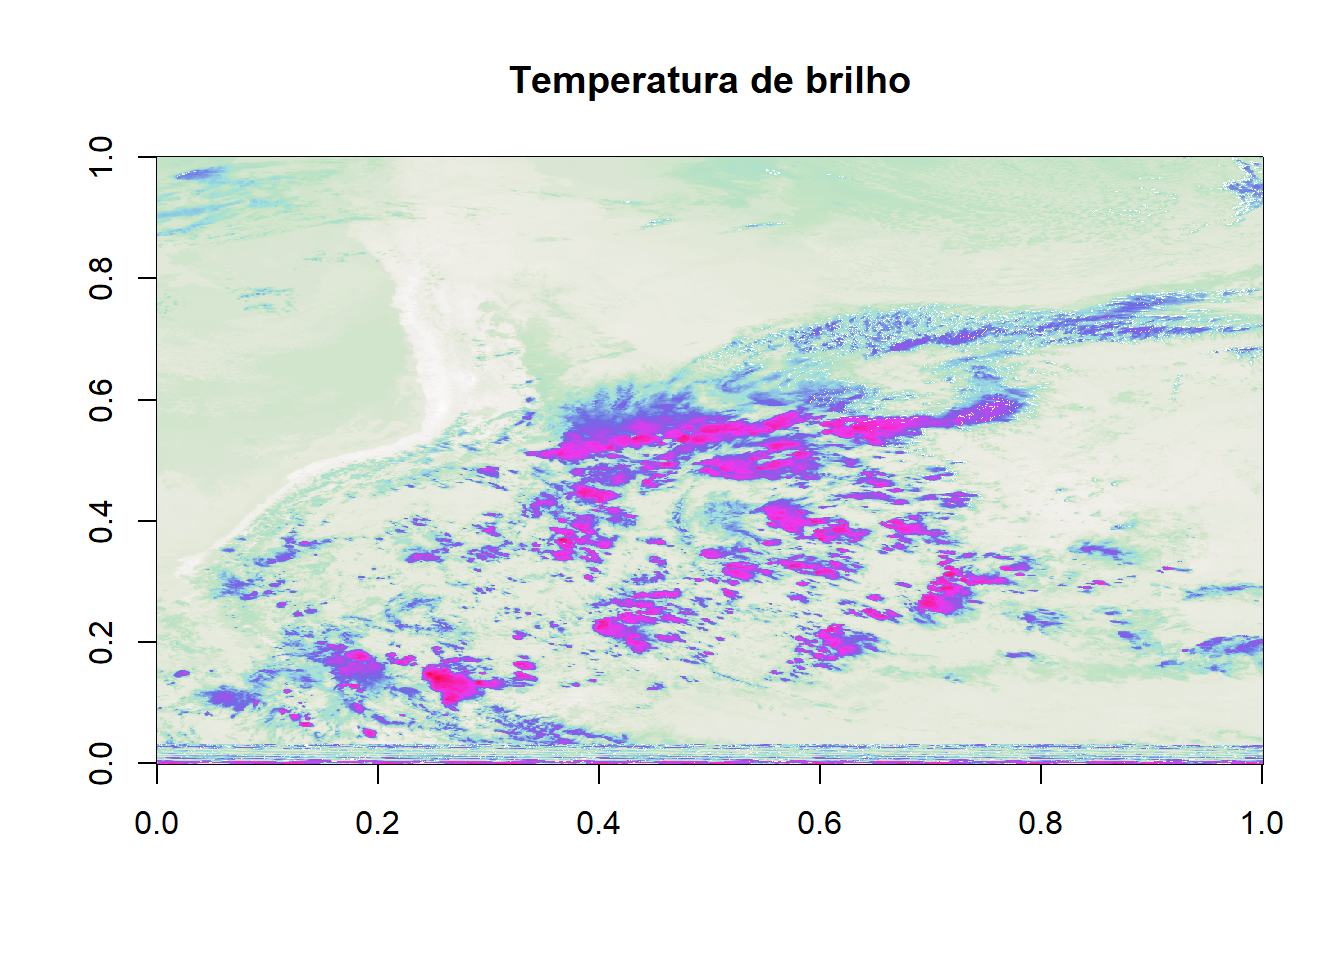
\includegraphics{cursoR_files/figure-latex/unnamed-chunk-79-1.pdf}

Tem algo estranho com esta imagem. O que é? (valendo um sticker).

\begin{Shaded}
\begin{Highlighting}[]
\KeywordTok{library}\NormalTok{(raster, }\DataTypeTok{quietly =} \OtherTok{TRUE}\NormalTok{)}
\NormalTok{l3 <-}\StringTok{ }\KeywordTok{raster}\NormalTok{(}\KeywordTok{t}\NormalTok{(l2[}\DecValTok{1}\OperatorTok{:}\DecValTok{1349}\NormalTok{,}\DecValTok{1}\OperatorTok{:}\DecValTok{1613}\NormalTok{]),}
                     \DataTypeTok{xmn=}\OperatorTok{-}\FloatTok{82.00}\NormalTok{,}
                     \DataTypeTok{ymn=}\OperatorTok{-}\FloatTok{44.96}\NormalTok{,}
                     \DataTypeTok{xmx=}\OperatorTok{-}\FloatTok{82.0}  \OperatorTok{+}\StringTok{ }\NormalTok{(}\FloatTok{0.03593245}\OperatorTok{*}\DecValTok{1349}\NormalTok{), }
                     \DataTypeTok{ymx=}\OperatorTok{-}\FloatTok{44.96} \OperatorTok{+}\StringTok{ }\NormalTok{(}\FloatTok{0.03593245}\OperatorTok{*}\DecValTok{1613}\NormalTok{),}
                     \DataTypeTok{crs =} \KeywordTok{CRS}\NormalTok{(}\StringTok{"+init=epsg:4326"}\NormalTok{))}
\KeywordTok{class}\NormalTok{(l3)}
\end{Highlighting}
\end{Shaded}

\begin{verbatim}
## [1] "RasterLayer"
## attr(,"package")
## [1] "raster"
\end{verbatim}

O capítulo geoespacial será visto no final deste curso. Porém, nesta
etapa vamos usar o pacote \texttt{raster} somente para analisar se os
dados binários foram lidos corretamente.

\begin{Shaded}
\begin{Highlighting}[]
\NormalTok{sp}\OperatorTok{::}\KeywordTok{spplot}\NormalTok{(((l3 }\OperatorTok{+}\StringTok{ }\DecValTok{75}\NormalTok{)}\OperatorTok{/}\DecValTok{100}\NormalTok{)}\OperatorTok{-}\DecValTok{273}\NormalTok{, }\CommentTok{# Estas correções são necessárias. Veja: http://www.cpc.ncep.noaa.gov/products/global_precip/html/README}
           \DataTypeTok{col.regions =} \KeywordTok{cpt}\NormalTok{(}\KeywordTok{find_cpt}\NormalTok{(}\StringTok{"sat"}\NormalTok{)[}\DecValTok{8}\NormalTok{]),}
           \DataTypeTok{at =} \KeywordTok{seq}\NormalTok{(}\OperatorTok{-}\DecValTok{80}\NormalTok{,}\DecValTok{0}\NormalTok{,}\DecValTok{1}\NormalTok{),}
           \DataTypeTok{main =} \StringTok{"Temperatura de brilho (ºC)"}\NormalTok{) }
\end{Highlighting}
\end{Shaded}

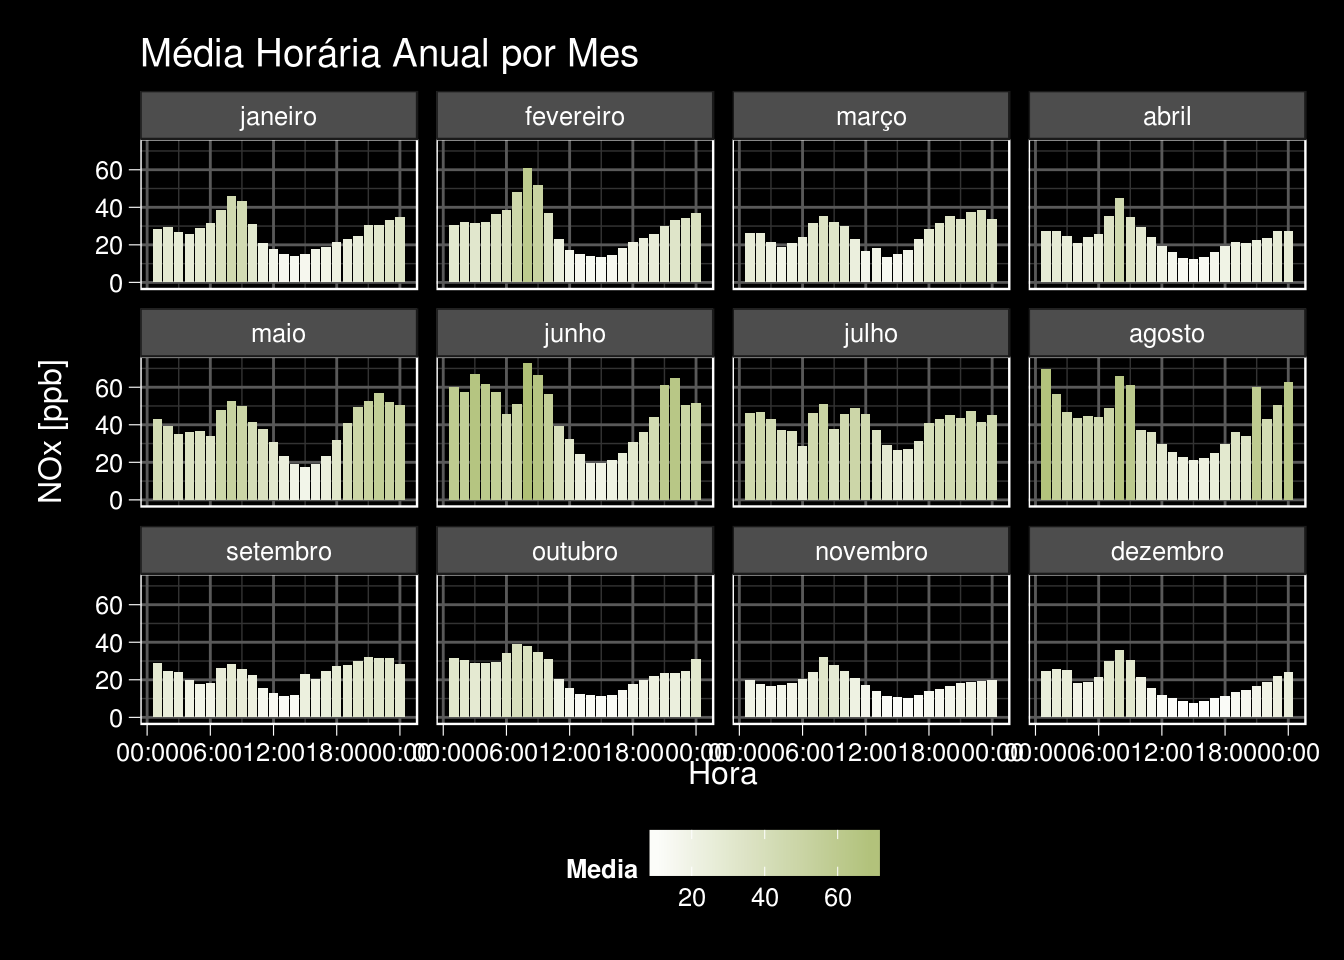
\includegraphics{cursoR_files/figure-latex/unnamed-chunk-81-1.pdf}

\textbf{Escrever dados binários no R}

\begin{Shaded}
\begin{Highlighting}[]
\CommentTok{# Escrever um arquivo binário: writeBin}
\KeywordTok{args}\NormalTok{(writeBin)}
\end{Highlighting}
\end{Shaded}

\begin{verbatim}
## function (object, con, size = NA_integer_, endian = .Platform$endian, 
##     useBytes = FALSE) 
## NULL
\end{verbatim}

\begin{Shaded}
\begin{Highlighting}[]
\CommentTok{# Lembre-se de usar ?writeBin}

\CommentTok{# Na linha abaixo vamos criar um arquivo temporário com o auxílio da função "tempfile" }
\CommentTok{# para depois escrever os dados dentro deste arquivo.}
\NormalTok{tf <-}\StringTok{ }\KeywordTok{tempfile}\NormalTok{()}
\CommentTok{# Vamos atribuir a "tb" os 20 primeiros valores de l1 (temperatura de brilho).}
\NormalTok{tb <-}\StringTok{ }\KeywordTok{c}\NormalTok{(}\DecValTok{21000}\NormalTok{, }\DecValTok{21000}\NormalTok{, }\DecValTok{20800}\NormalTok{, }\DecValTok{21000}\NormalTok{, }\DecValTok{20800}\NormalTok{, }\DecValTok{20700}\NormalTok{, }\DecValTok{20600}\NormalTok{, }\DecValTok{20600}\NormalTok{, }\DecValTok{20900}\NormalTok{, }\DecValTok{20900}\NormalTok{, }
        \DecValTok{20900}\NormalTok{, }\DecValTok{20900}\NormalTok{, }\DecValTok{20700}\NormalTok{, }\DecValTok{20500}\NormalTok{, }\DecValTok{20500}\NormalTok{, }\DecValTok{20400}\NormalTok{, }\DecValTok{20500}\NormalTok{, }\DecValTok{20700}\NormalTok{, }\DecValTok{20400}\NormalTok{, }\DecValTok{20300}\NormalTok{)}
\KeywordTok{class}\NormalTok{(tb)}
\end{Highlighting}
\end{Shaded}

\begin{verbatim}
## [1] "numeric"
\end{verbatim}

\begin{Shaded}
\begin{Highlighting}[]
\NormalTok{x <-}\StringTok{ }\KeywordTok{as.integer}\NormalTok{(tb)}
\KeywordTok{writeBin}\NormalTok{(x, }\DataTypeTok{con =}\NormalTok{ tf)}

\CommentTok{# Agora vamos ler o arquivo binário escrito acima. Você lembra quais são os argumentos para ler binário?}
\KeywordTok{readBin}\NormalTok{(tf,}
        \DataTypeTok{what =} \StringTok{"integer"}\NormalTok{,}
        \DataTypeTok{n =} \DecValTok{20}\NormalTok{)}
\end{Highlighting}
\end{Shaded}

\begin{verbatim}
##  [1] 21000 21000 20800 21000 20800 20700 20600 20600 20900 20900 20900
## [12] 20900 20700 20500 20500 20400 20500 20700 20400 20300
\end{verbatim}

\chapter{Plotando}\label{plotando}

\section{\texorpdfstring{\texttt{plot}
(base)}{plot (base)}}\label{plot-base}

\textbf{Exemplo}: Dados de qualidade do ar

\begin{Shaded}
\begin{Highlighting}[]
\NormalTok{df <-}\StringTok{ }\KeywordTok{readRDS}\NormalTok{(}\StringTok{"dados/df.rds"}\NormalTok{)}
\KeywordTok{summary}\NormalTok{(df)}
\end{Highlighting}
\end{Shaded}

\begin{verbatim}
## Warning in as.POSIXlt.POSIXct(x, tz): unknown timezone 'Americas/Sao_Paulo'
\end{verbatim}

\begin{verbatim}
##        TipodeRede   TipodeMonitoramento               Tipo     
##  Automático:8581   CETESB:8581         Dados Primários:8581  
##                                                                
##                                                                
##                                                                
##                                                                
##                                                                
##                                                                
##          Data           Hora      CodigoEstaÃ.Ã.o
##  01/01/2014:  24   16:00  : 363   Min.   :95     
##  01/01/2015:  24   12:00  : 361   1st Qu.:95     
##  01/02/2014:  24   14:00  : 361   Median :95     
##  01/04/2014:  24   18:00  : 361   Mean   :95     
##  01/05/2014:  24   13:00  : 360   3rd Qu.:95     
##  01/06/2014:  24   17:00  : 360   Max.   :95     
##  (Other)   :8437   (Other):6415                  
##                      NomeEstaÃ.Ã.o                       NomeParÃ.metro
##  Cid.Universitária-USP-Ipen:8581   NOx (Óxidos de Nitrogênio):8581  
##                                                                        
##                                                                        
##                                                                        
##                                                                        
##                                                                        
##                                                                        
##  UnidadedeMedida  MediaHoraria    MediaMovel  Valido    
##  ppb:8581        Min.   :  0.00   -:8581     Não: 907  
##                  1st Qu.:  9.00              Sim :7674  
##                  Median : 18.00                         
##                  Mean   : 29.87                         
##                  3rd Qu.: 34.00                         
##                  Max.   :306.00                         
##                  NA's   :260                            
##   tempo_char            tempo                       weekdays        
##  Length:8581        Min.   :2014-01-01 01:00:00   Length:8581       
##  Class :character   1st Qu.:2014-04-05 14:00:00   Class :character  
##  Mode  :character   Median :2014-07-05 23:00:00   Mode  :character  
##                     Mean   :2014-07-04 20:22:55                     
##                     3rd Qu.:2014-10-03 10:00:00                     
##                     Max.   :2015-01-02 00:00:00                     
##                                                                     
##      mes             diajuliano           ano           
##  Length:8581        Length:8581       Length:8581       
##  Class :character   Class :difftime   Class :character  
##  Mode  :character   Mode  :numeric    Mode  :character  
##                                                         
##                                                         
##                                                         
## 
\end{verbatim}

A função \texttt{plot} precisa dos seguintes argumentos:

\begin{Shaded}
\begin{Highlighting}[]
\KeywordTok{args}\NormalTok{(plot)}
\end{Highlighting}
\end{Shaded}

\begin{verbatim}
## function (x, y, ...) 
## NULL
\end{verbatim}

Então, a forma mais fácil de plotar uma variável em função do tempo é:

\begin{Shaded}
\begin{Highlighting}[]
\KeywordTok{plot}\NormalTok{(}\DataTypeTok{x =}\NormalTok{ df}\OperatorTok{$}\NormalTok{tempo, }\DataTypeTok{y =}\NormalTok{ df}\OperatorTok{$}\NormalTok{MediaHoraria)}
\end{Highlighting}
\end{Shaded}

\begin{verbatim}
## Warning in as.POSIXlt.POSIXct(z): unknown timezone 'Americas/Sao_Paulo'
\end{verbatim}

\begin{verbatim}
## Warning in as.POSIXct.POSIXlt(zz): unknown timezone 'Americas/Sao_Paulo'
\end{verbatim}

\begin{verbatim}
## Warning in as.POSIXlt.POSIXct(x, tz): unknown timezone 'Americas/Sao_Paulo'
\end{verbatim}

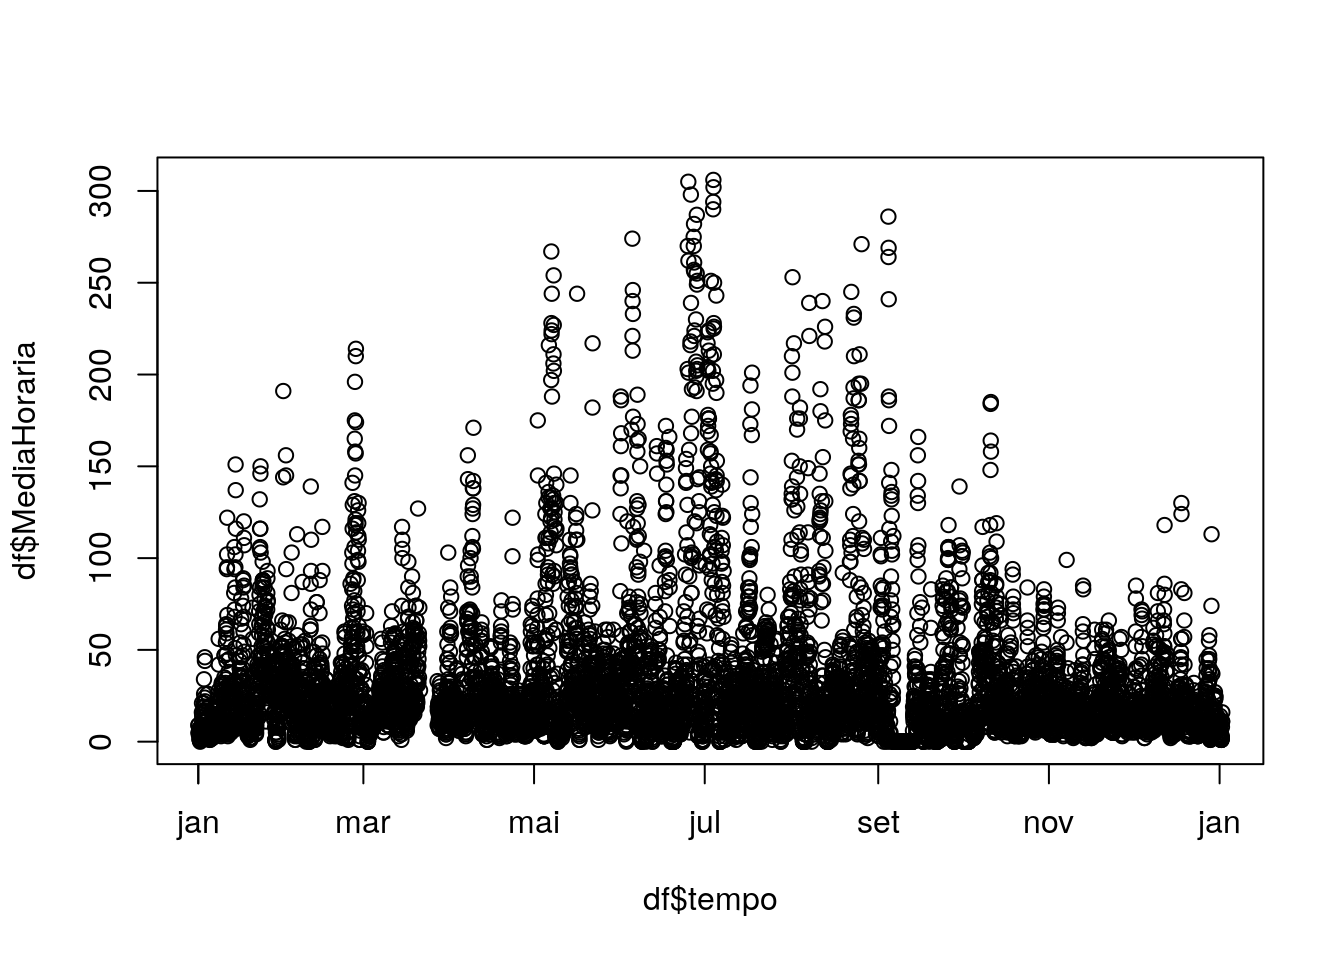
\includegraphics{cursoR_files/figure-latex/unnamed-chunk-85-1.pdf}

Feio, né?\\
Tentando deixar mais bonito\ldots{}

\begin{Shaded}
\begin{Highlighting}[]
\KeywordTok{plot}\NormalTok{(}\DataTypeTok{x =}\NormalTok{ df}\OperatorTok{$}\NormalTok{tempo[}\DecValTok{1}\OperatorTok{:}\DecValTok{100}\NormalTok{], }\DataTypeTok{y =}\NormalTok{ df}\OperatorTok{$}\NormalTok{MediaHoraria[}\DecValTok{1}\OperatorTok{:}\DecValTok{100}\NormalTok{], }\CommentTok{#-- Selecionando uma parte do df!}
     \DataTypeTok{pch =} \DecValTok{16}\NormalTok{, }\CommentTok{#-- Forma do ponto (círculo preenchido)}
     \DataTypeTok{type =} \StringTok{"b"}\NormalTok{, }\CommentTok{#-- Tipo de gráfico ("b" = both, ponto e linha)}
     \DataTypeTok{col =} \StringTok{"blue"}\NormalTok{, }\CommentTok{#-- Cor do elemento (definido pelo type)}
     \DataTypeTok{xlab =} \StringTok{"Data"}\NormalTok{, }\DataTypeTok{ylab =} \StringTok{"NOx [ppb]"}\NormalTok{, }\CommentTok{#-- Nome dos eixos x e y}
     \DataTypeTok{main =} \StringTok{"Gráfico mais Bonito"}\NormalTok{) }\CommentTok{#-- Título do gráfico}
\end{Highlighting}
\end{Shaded}

\begin{verbatim}
## Warning in as.POSIXlt.POSIXct(x): unknown timezone 'Americas/Sao_Paulo'
\end{verbatim}

\begin{verbatim}
## Warning in as.POSIXct.POSIXlt(round(z, "days")): unknown timezone
## 'Americas/Sao_Paulo'
\end{verbatim}

\begin{verbatim}
## Warning in as.POSIXlt.POSIXct(x, tz): unknown timezone 'Americas/Sao_Paulo'
\end{verbatim}

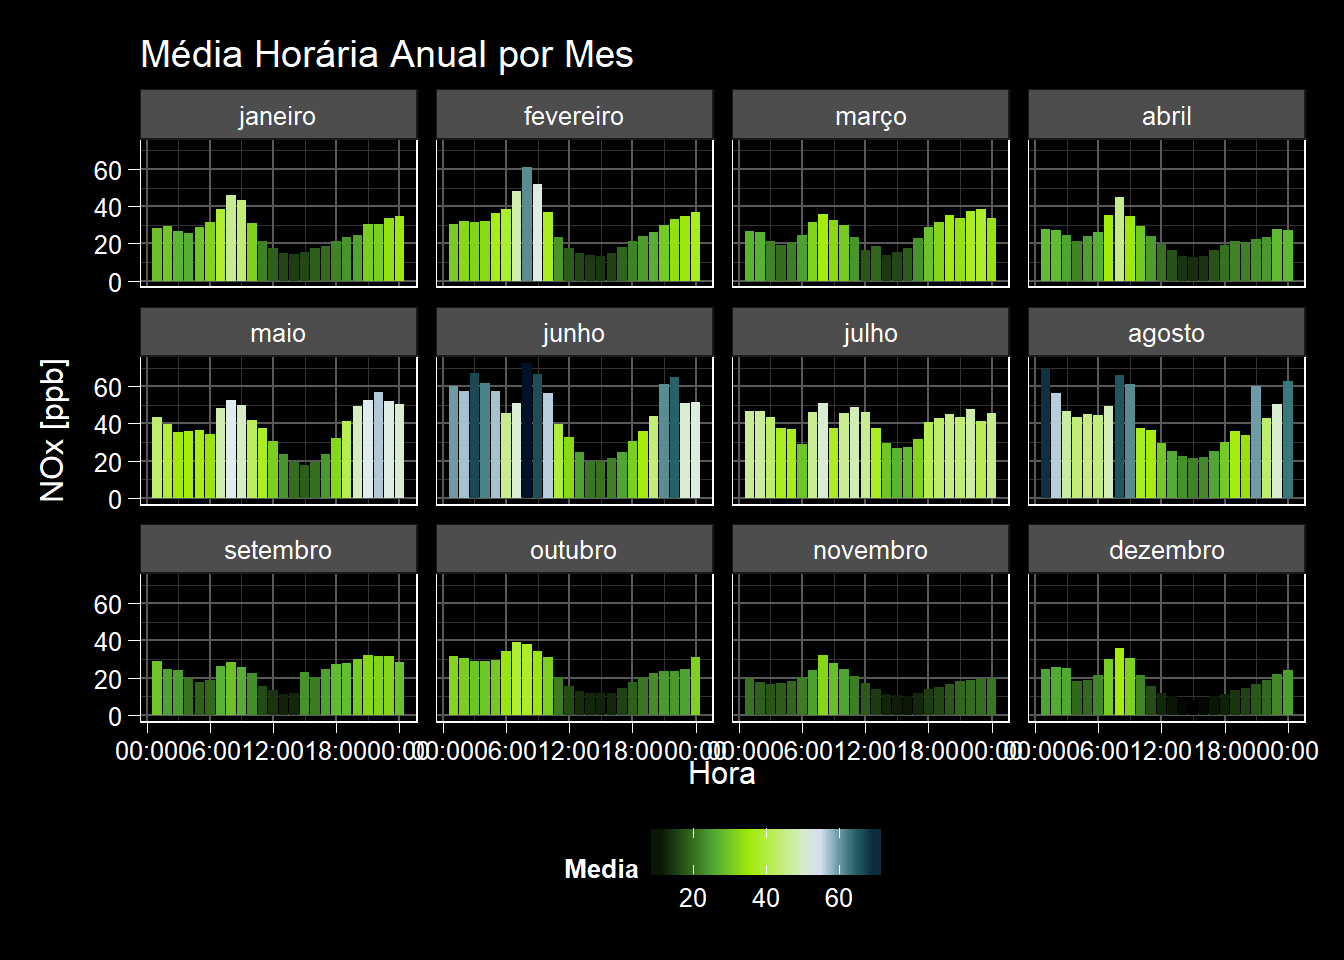
\includegraphics{cursoR_files/figure-latex/unnamed-chunk-86-1.pdf}

Colocando \textbf{DOIS} elementos no mesmo gráfico:

\begin{Shaded}
\begin{Highlighting}[]
\NormalTok{df_parcial <-}\StringTok{ }\NormalTok{df[}\DecValTok{1}\OperatorTok{:}\DecValTok{180}\NormalTok{,] }\CommentTok{#-- Selecionando uma parte do df!}
\KeywordTok{plot}\NormalTok{(}\DataTypeTok{x =}\NormalTok{ df_parcial}\OperatorTok{$}\NormalTok{tempo[df_parcial}\OperatorTok{$}\NormalTok{Valido }\OperatorTok{==}\StringTok{ "Sim"}\NormalTok{], }
     \DataTypeTok{y =}\NormalTok{ df_parcial}\OperatorTok{$}\NormalTok{MediaHoraria[df_parcial}\OperatorTok{$}\NormalTok{Valido }\OperatorTok{==}\StringTok{ "Sim"}\NormalTok{],}
     \DataTypeTok{pch =} \DecValTok{16}\NormalTok{, }\DataTypeTok{type =} \StringTok{"b"}\NormalTok{, }\DataTypeTok{col =} \StringTok{"blue"}\NormalTok{,}
     \DataTypeTok{xlab =} \StringTok{"Data"}\NormalTok{, }\DataTypeTok{ylab =} \StringTok{"NOx [ppb]"}\NormalTok{,}
     \DataTypeTok{main =} \StringTok{"Dados Válidos e Inválidos"}\NormalTok{)}
\end{Highlighting}
\end{Shaded}

\begin{verbatim}
## Warning in as.POSIXlt.POSIXct(x): unknown timezone 'Americas/Sao_Paulo'
\end{verbatim}

\begin{verbatim}
## Warning in as.POSIXct.POSIXlt(round(z, "days")): unknown timezone
## 'Americas/Sao_Paulo'
\end{verbatim}

\begin{verbatim}
## Warning in as.POSIXlt.POSIXct(x, tz): unknown timezone 'Americas/Sao_Paulo'
\end{verbatim}

\begin{Shaded}
\begin{Highlighting}[]
\KeywordTok{lines}\NormalTok{(}\DataTypeTok{x =}\NormalTok{ df_parcial}\OperatorTok{$}\NormalTok{tempo[df}\OperatorTok{$}\NormalTok{Valido }\OperatorTok{==}\StringTok{ "Não"}\NormalTok{], }
      \DataTypeTok{y =}\NormalTok{ df_parcial}\OperatorTok{$}\NormalTok{MediaHoraria[df}\OperatorTok{$}\NormalTok{Valido }\OperatorTok{==}\StringTok{ "Não"}\NormalTok{], }
      \DataTypeTok{pch =} \DecValTok{15}\NormalTok{, }\DataTypeTok{type =} \StringTok{"b"}\NormalTok{, }\DataTypeTok{col =} \StringTok{"red"}\NormalTok{)}
\end{Highlighting}
\end{Shaded}

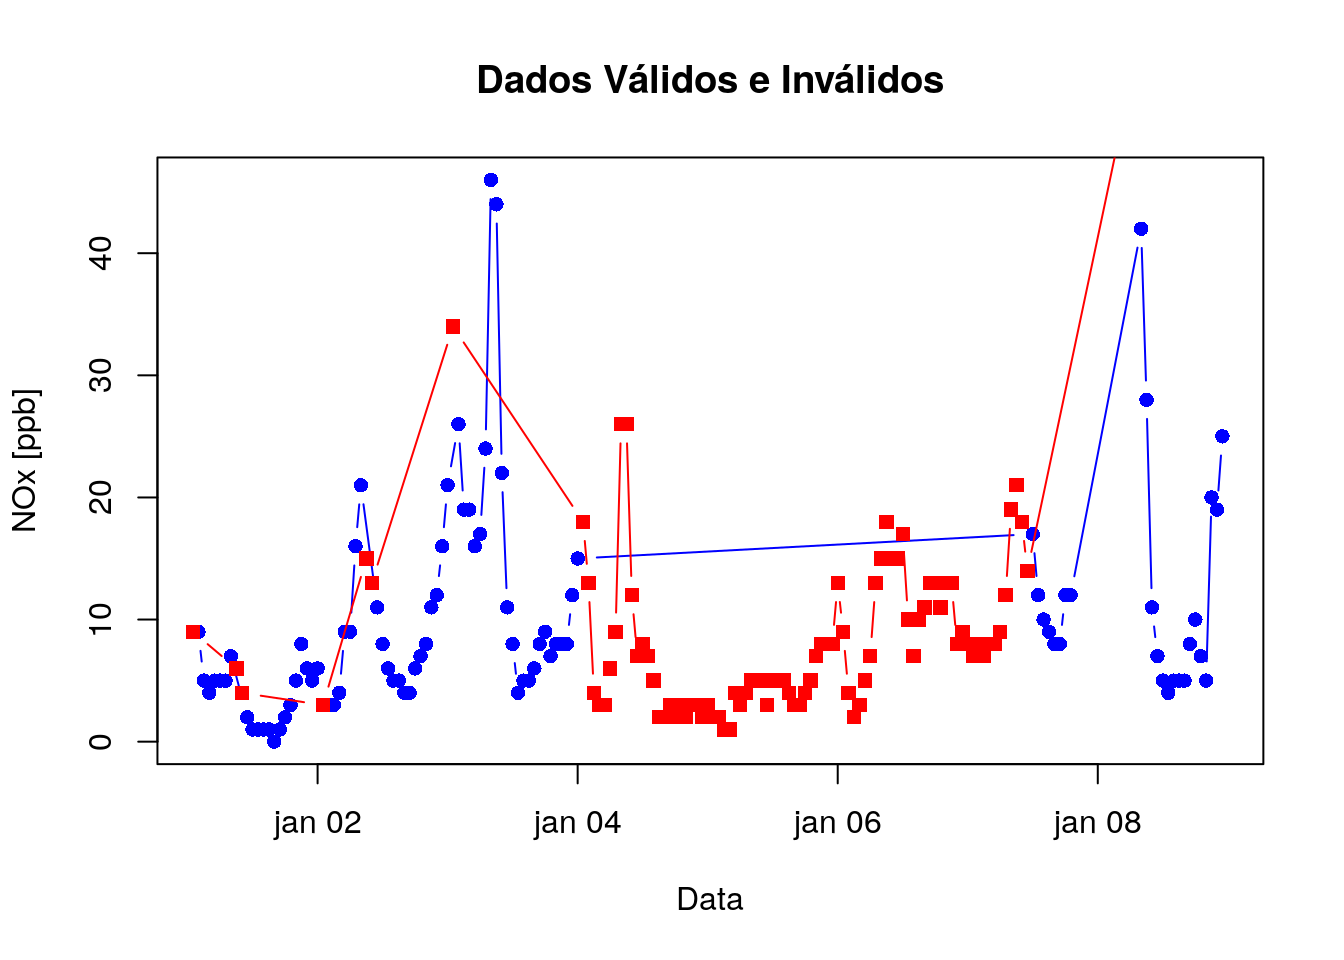
\includegraphics{cursoR_files/figure-latex/unnamed-chunk-87-1.pdf}

\begin{center}\rule{0.5\linewidth}{\linethickness}\end{center}

{\textbf{Desafio}: Coloque uma legenda na figura especificando que os
dados válidos estão em azul e os inválidos em vermelho }

\begin{center}\rule{0.5\linewidth}{\linethickness}\end{center}

A função \texttt{plot} cumpre bem o papel de gerar um gráfico simples, e
até permite algumas customizações, mas ela exige cada vez mais linhas de
código e argumentos dentro das funções para deixar o gráfico ``mais
bonito'' - ao cumprir o desafio, você irá perceber como uma coisa
``simples'' como colocar uma legenda pode exigir muito mais do que
parece!

\section{\texorpdfstring{\texttt{ggplot}
(ggplot2)}{ggplot (ggplot2)}}\label{ggplot-ggplot2}

A função \texttt{ggplot} funciona de um jeito um pouco diferente. Veja a
figura abaixo:

\begin{figure}
\centering
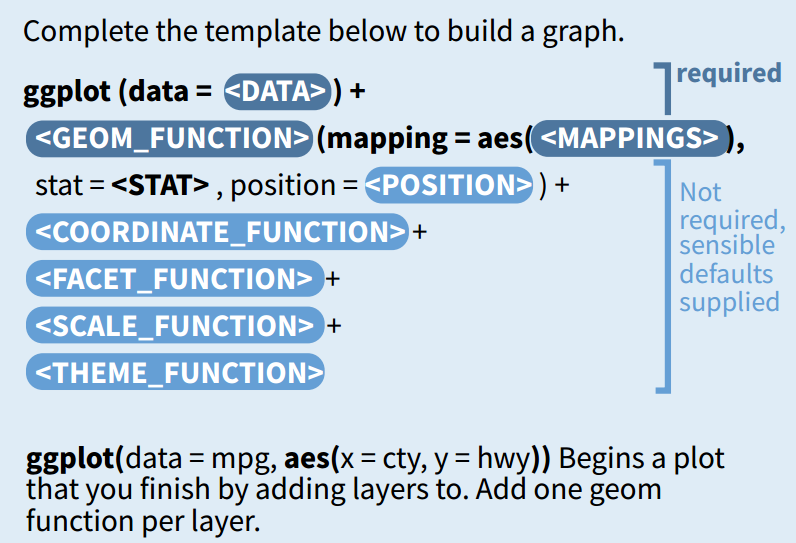
\includegraphics{figuras/ggplot_guide.png}
\caption{Fonte:
\url{https://github.com/rstudio/cheatsheets/raw/master/data-visualization-2.1.pdf}}
\end{figure}

Em vez de uma única função, o gráfico é formado por camadas, sendo que
cada camada é um elemento (\texttt{geom\_...} ou \texttt{stat\_...}) ou
configuração (\texttt{scale\_...\_...}, \texttt{coord\_...},
\texttt{theme} ou \texttt{theme\_...}, \texttt{guides}, \texttt{labs},
etc). Consulte a maioria das opções disponíveis em
\href{https://github.com/rstudio/cheatsheets/raw/master/data-visualization-2.1.pdf}{Data
Visualization Cheatsheet}.

Que tal refazermos os gráficos da seção anterior?

\begin{Shaded}
\begin{Highlighting}[]
\CommentTok{#-- Não esqueça de carregar o pacote!}
\KeywordTok{library}\NormalTok{(ggplot2)}
\end{Highlighting}
\end{Shaded}

\begin{Shaded}
\begin{Highlighting}[]
\KeywordTok{ggplot}\NormalTok{(df, }\KeywordTok{aes}\NormalTok{(}\DataTypeTok{x =}\NormalTok{ tempo, }\DataTypeTok{y =}\NormalTok{ MediaHoraria)) }\OperatorTok{+}
\StringTok{  }\KeywordTok{geom_point}\NormalTok{(}\DataTypeTok{pch =} \DecValTok{1}\NormalTok{)}
\end{Highlighting}
\end{Shaded}

\begin{verbatim}
## Warning in as.POSIXlt.POSIXct(x): unknown timezone 'Americas/Sao_Paulo'
\end{verbatim}

\begin{verbatim}
## Warning in as.POSIXct.POSIXlt(from): unknown timezone 'Americas/Sao_Paulo'
\end{verbatim}

\begin{verbatim}
## Warning in as.POSIXlt.POSIXct(to): unknown timezone 'Americas/Sao_Paulo'
\end{verbatim}

\begin{verbatim}
## Warning in as.POSIXct.POSIXlt(r1): unknown timezone 'Americas/Sao_Paulo'
\end{verbatim}

\begin{verbatim}
## Warning in as.POSIXlt.POSIXct(from): unknown timezone 'Americas/Sao_Paulo'
\end{verbatim}

\begin{verbatim}
## Warning in as.POSIXct.POSIXlt(r1): unknown timezone 'Americas/Sao_Paulo'
\end{verbatim}

\begin{verbatim}
## Warning in as.POSIXlt.POSIXct(x): unknown timezone 'Americas/Sao_Paulo'
\end{verbatim}

\begin{verbatim}
## Warning in as.POSIXct.POSIXlt(from): unknown timezone 'Americas/Sao_Paulo'
\end{verbatim}

\begin{verbatim}
## Warning in as.POSIXlt.POSIXct(to): unknown timezone 'Americas/Sao_Paulo'
\end{verbatim}

\begin{verbatim}
## Warning in as.POSIXct.POSIXlt(r1): unknown timezone 'Americas/Sao_Paulo'
\end{verbatim}

\begin{verbatim}
## Warning in as.POSIXlt.POSIXct(from): unknown timezone 'Americas/Sao_Paulo'
\end{verbatim}

\begin{verbatim}
## Warning in as.POSIXct.POSIXlt(r1): unknown timezone 'Americas/Sao_Paulo'
\end{verbatim}

\begin{verbatim}
## Warning in as.POSIXlt.POSIXct(x, tz): unknown timezone 'Americas/Sao_Paulo'
\end{verbatim}

\begin{verbatim}
## Warning: Removed 260 rows containing missing values (geom_point).
\end{verbatim}

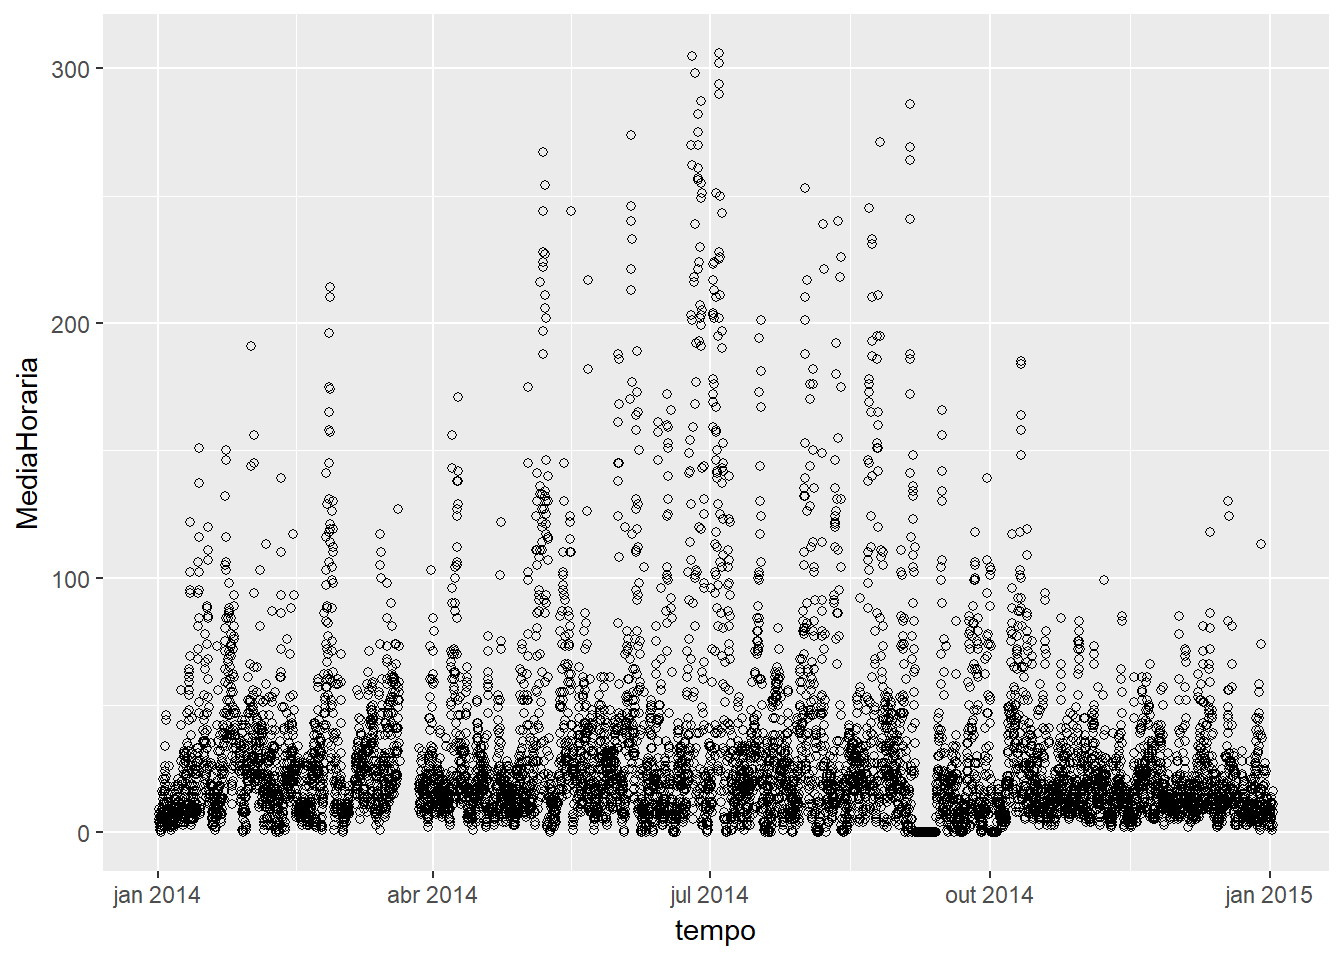
\includegraphics{cursoR_files/figure-latex/unnamed-chunk-89-1.pdf}

\begin{Shaded}
\begin{Highlighting}[]
\KeywordTok{ggplot}\NormalTok{(df[}\DecValTok{1}\OperatorTok{:}\DecValTok{100}\NormalTok{,], }\KeywordTok{aes}\NormalTok{(}\DataTypeTok{x =}\NormalTok{ tempo, }\DataTypeTok{y =}\NormalTok{ MediaHoraria)) }\OperatorTok{+}\StringTok{ }
\StringTok{  }\KeywordTok{geom_line}\NormalTok{(}\DataTypeTok{color =} \StringTok{"blue"}\NormalTok{) }\OperatorTok{+}\StringTok{ }\CommentTok{#-- Linhas...}
\StringTok{  }\KeywordTok{geom_point}\NormalTok{(}\DataTypeTok{color =} \StringTok{"blue"}\NormalTok{, }\DataTypeTok{pch =} \DecValTok{16}\NormalTok{) }\OperatorTok{+}\StringTok{ }\CommentTok{#-- ... com pontos}
\StringTok{  }\KeywordTok{labs}\NormalTok{(}\DataTypeTok{title =} \StringTok{"Gráfico mais Bonito"}\NormalTok{, }\DataTypeTok{x =} \StringTok{"Data"}\NormalTok{, }\DataTypeTok{y =} \StringTok{"NOx [ppb]"}\NormalTok{) }\OperatorTok{+}\StringTok{ }\CommentTok{#-- Títulos}
\StringTok{  }\KeywordTok{theme}\NormalTok{(}\DataTypeTok{plot.title =} \KeywordTok{element_text}\NormalTok{(}\DataTypeTok{hjust =} \FloatTok{0.5}\NormalTok{)) }\CommentTok{#-- Centralizando o título}
\end{Highlighting}
\end{Shaded}

\begin{verbatim}
## Warning in as.POSIXlt.POSIXct(x): unknown timezone 'Americas/Sao_Paulo'
\end{verbatim}

\begin{verbatim}
## Warning in as.POSIXct.POSIXlt(from): unknown timezone 'Americas/Sao_Paulo'

## Warning in as.POSIXct.POSIXlt(from): unknown timezone 'Americas/Sao_Paulo'
\end{verbatim}

\begin{verbatim}
## Warning in as.POSIXct.POSIXlt(r1): unknown timezone 'Americas/Sao_Paulo'
\end{verbatim}

\begin{verbatim}
## Warning in as.POSIXlt.POSIXct(from): unknown timezone 'Americas/Sao_Paulo'
\end{verbatim}

\begin{verbatim}
## Warning in as.POSIXct.POSIXlt(r1): unknown timezone 'Americas/Sao_Paulo'
\end{verbatim}

\begin{verbatim}
## Warning in as.POSIXlt.POSIXct(x): unknown timezone 'Americas/Sao_Paulo'
\end{verbatim}

\begin{verbatim}
## Warning in as.POSIXct.POSIXlt(from): unknown timezone 'Americas/Sao_Paulo'

## Warning in as.POSIXct.POSIXlt(from): unknown timezone 'Americas/Sao_Paulo'
\end{verbatim}

\begin{verbatim}
## Warning in as.POSIXct.POSIXlt(r1): unknown timezone 'Americas/Sao_Paulo'
\end{verbatim}

\begin{verbatim}
## Warning in as.POSIXlt.POSIXct(from): unknown timezone 'Americas/Sao_Paulo'
\end{verbatim}

\begin{verbatim}
## Warning in as.POSIXct.POSIXlt(r1): unknown timezone 'Americas/Sao_Paulo'
\end{verbatim}

\begin{verbatim}
## Warning in as.POSIXlt.POSIXct(x, tz): unknown timezone 'Americas/Sao_Paulo'
\end{verbatim}

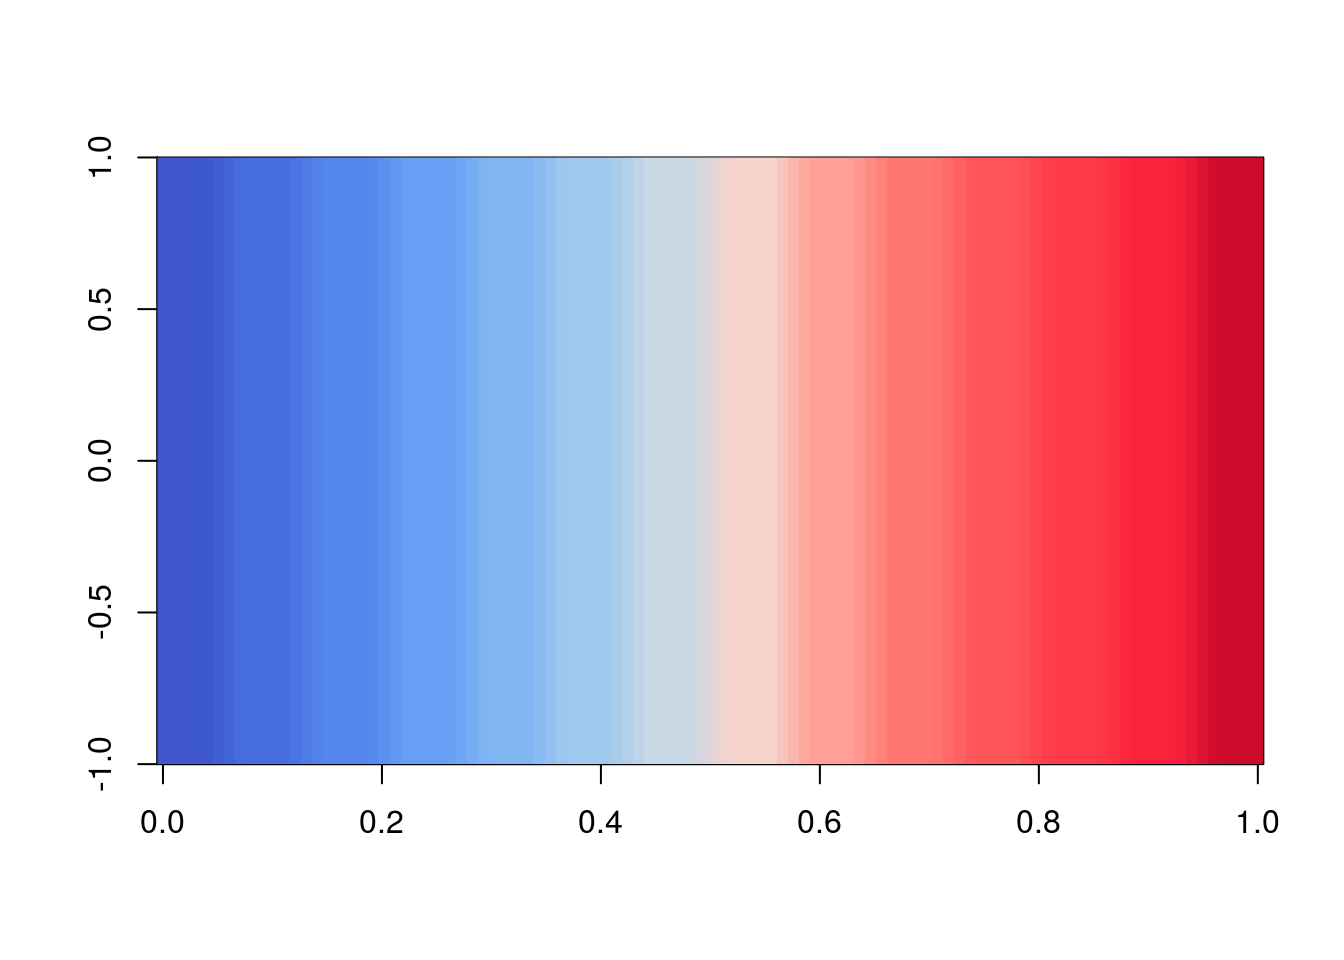
\includegraphics{cursoR_files/figure-latex/unnamed-chunk-90-1.pdf}

Agora o mais interessante:

\begin{Shaded}
\begin{Highlighting}[]
\KeywordTok{ggplot}\NormalTok{(df[}\DecValTok{1}\OperatorTok{:}\DecValTok{180}\NormalTok{,], }\KeywordTok{aes}\NormalTok{(}\DataTypeTok{x =}\NormalTok{ tempo, }\DataTypeTok{y =}\NormalTok{ MediaHoraria)) }\OperatorTok{+}\StringTok{ }
\StringTok{  }\KeywordTok{geom_line}\NormalTok{(}\KeywordTok{aes}\NormalTok{(}\DataTypeTok{color =}\NormalTok{ Valido)) }\OperatorTok{+}
\StringTok{  }\KeywordTok{geom_point}\NormalTok{(}\KeywordTok{aes}\NormalTok{(}\DataTypeTok{color =}\NormalTok{ Valido, }\DataTypeTok{shape =}\NormalTok{ Valido)) }\OperatorTok{+}
\StringTok{  }\KeywordTok{labs}\NormalTok{(}\DataTypeTok{title =} \StringTok{"Dados Válidos e Inválidos"}\NormalTok{, }\DataTypeTok{x =} \StringTok{"Data"}\NormalTok{, }\DataTypeTok{y =} \StringTok{"NOx [ppb]"}\NormalTok{) }\OperatorTok{+}
\StringTok{  }\KeywordTok{scale_color_manual}\NormalTok{(}\DataTypeTok{values =} \KeywordTok{c}\NormalTok{(}\StringTok{"red"}\NormalTok{, }\StringTok{"blue"}\NormalTok{)) }\OperatorTok{+}\StringTok{ }\CommentTok{#-- Definindo as cores manualmente}
\StringTok{  }\KeywordTok{scale_shape_manual}\NormalTok{(}\DataTypeTok{values =} \KeywordTok{c}\NormalTok{(}\DecValTok{15}\NormalTok{, }\DecValTok{16}\NormalTok{)) }\OperatorTok{+}\StringTok{ }\CommentTok{#-- Definindo as formas manualmente}
\StringTok{  }\KeywordTok{theme}\NormalTok{(}\DataTypeTok{plot.title =} \KeywordTok{element_text}\NormalTok{(}\DataTypeTok{hjust =} \FloatTok{0.5}\NormalTok{))}
\end{Highlighting}
\end{Shaded}

\begin{verbatim}
## Warning in as.POSIXlt.POSIXct(x): unknown timezone 'Americas/Sao_Paulo'
\end{verbatim}

\begin{verbatim}
## Warning in as.POSIXct.POSIXlt(from): unknown timezone 'Americas/Sao_Paulo'

## Warning in as.POSIXct.POSIXlt(from): unknown timezone 'Americas/Sao_Paulo'
\end{verbatim}

\begin{verbatim}
## Warning in as.POSIXct.POSIXlt(r1): unknown timezone 'Americas/Sao_Paulo'
\end{verbatim}

\begin{verbatim}
## Warning in as.POSIXlt.POSIXct(from): unknown timezone 'Americas/Sao_Paulo'
\end{verbatim}

\begin{verbatim}
## Warning in as.POSIXct.POSIXlt(r1): unknown timezone 'Americas/Sao_Paulo'
\end{verbatim}

\begin{verbatim}
## Warning in as.POSIXlt.POSIXct(x, tz): unknown timezone 'Americas/Sao_Paulo'
\end{verbatim}

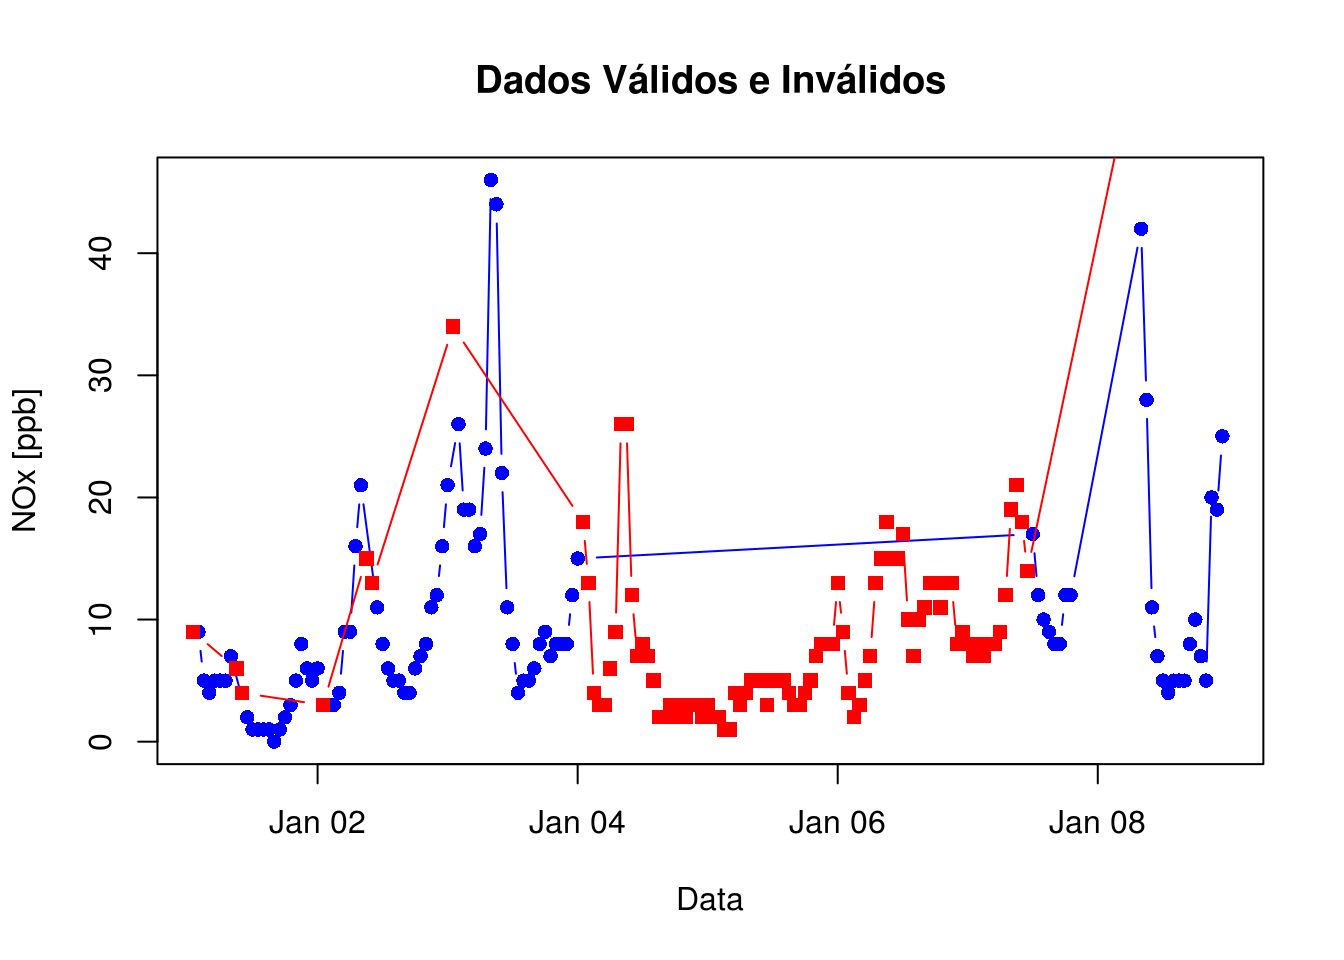
\includegraphics{cursoR_files/figure-latex/unnamed-chunk-91-1.pdf}

{\textbf{Pergunta}: Qual a principal diferença entre o código acima e o
\protect\hyperlink{plot_base}{código usando \texttt{plot}}?}

A função \texttt{ggplot} plota apenas data frames, pois ela mapeia as
variáveis por nomes de colunas. Assim, é preciso
\protect\hyperlink{convert_df}{converter matrizes ou arrays em data
frames}.\\
Uma vantagem de trabalharmos com data frames,
\protect\hyperlink{processing_dfs}{como já vimos antes}, é poder
manipular esses dados de muitas formas possíveis antes de plotá-los.

\textbf{Continuação do Exemplo}: Extraindo algumas informações sobre os
dados

Vamos analisar o ano de 2014:

\begin{itemize}
\tightlist
\item
  \emph{Em média}, como o NOx varia ao longo do dia?

  \begin{itemize}
  \tightlist
  \item
    E para cada dia da semana?\\
  \item
    E para cada mês?
  \end{itemize}
\end{itemize}

Usando algumas outras funções dentro do
\protect\hyperlink{tidyverse}{\textbf{Tidyverse}}:

\begin{Shaded}
\begin{Highlighting}[]
\KeywordTok{library}\NormalTok{(tidyverse)}

\NormalTok{df_}\DecValTok{2014}\NormalTok{ <-}\StringTok{ }\KeywordTok{filter}\NormalTok{(df, ano }\OperatorTok{==}\StringTok{ "2014"}\NormalTok{)}
\NormalTok{df_2014_hour <-}\StringTok{ }\NormalTok{df_}\DecValTok{2014} \OperatorTok\StringTok{ }\CommentTok{#-- A partir do data frame df_2014}
\StringTok{  }\KeywordTok{group_by}\NormalTok{(Hora) }\OperatorTok\StringTok{ }\CommentTok{#-- Agrupe os dados pela coluna hora}
\StringTok{  }\KeywordTok{summarise}\NormalTok{(}\DataTypeTok{Media =} \KeywordTok{mean}\NormalTok{(MediaHoraria, }\DataTypeTok{na.rm =}\NormalTok{ T)) }\OperatorTok\StringTok{ }\CommentTok{#-- E calcule as médias, }
\StringTok{                                                       }\CommentTok{#-- salvando em uma coluna nova}
\StringTok{  }\KeywordTok{mutate}\NormalTok{(}\DataTypeTok{Hora =} \KeywordTok{as.POSIXct}\NormalTok{(}\KeywordTok{strptime}\NormalTok{(Hora, }\StringTok{"%H:%M"}\NormalTok{))) }\OperatorTok\StringTok{ }\CommentTok{#-- Transformando em data}
\StringTok{  }\KeywordTok{ungroup}\NormalTok{() }\CommentTok{#-- Desagrupando}

\KeywordTok{ggplot}\NormalTok{(df_2014_hour) }\OperatorTok{+}
\StringTok{  }\KeywordTok{scale_x_datetime}\NormalTok{(}\DataTypeTok{date_labels =} \StringTok{"%H:%M"}\NormalTok{) }\OperatorTok{+}\StringTok{ }\CommentTok{#-- Formato de data que aparecerá no eixo x}
\StringTok{  }\KeywordTok{geom_line}\NormalTok{(}\KeywordTok{aes}\NormalTok{(}\DataTypeTok{x =}\NormalTok{ Hora, }\DataTypeTok{y =}\NormalTok{ Media, }\DataTypeTok{group =} \DecValTok{1}\NormalTok{), }\DataTypeTok{color =} \StringTok{"purple"}\NormalTok{) }\OperatorTok{+}
\StringTok{  }\KeywordTok{labs}\NormalTok{(}\DataTypeTok{title =} \StringTok{"Média Horária Anual"}\NormalTok{, }\DataTypeTok{y =} \StringTok{"NOx [ppb]"}\NormalTok{)}
\end{Highlighting}
\end{Shaded}

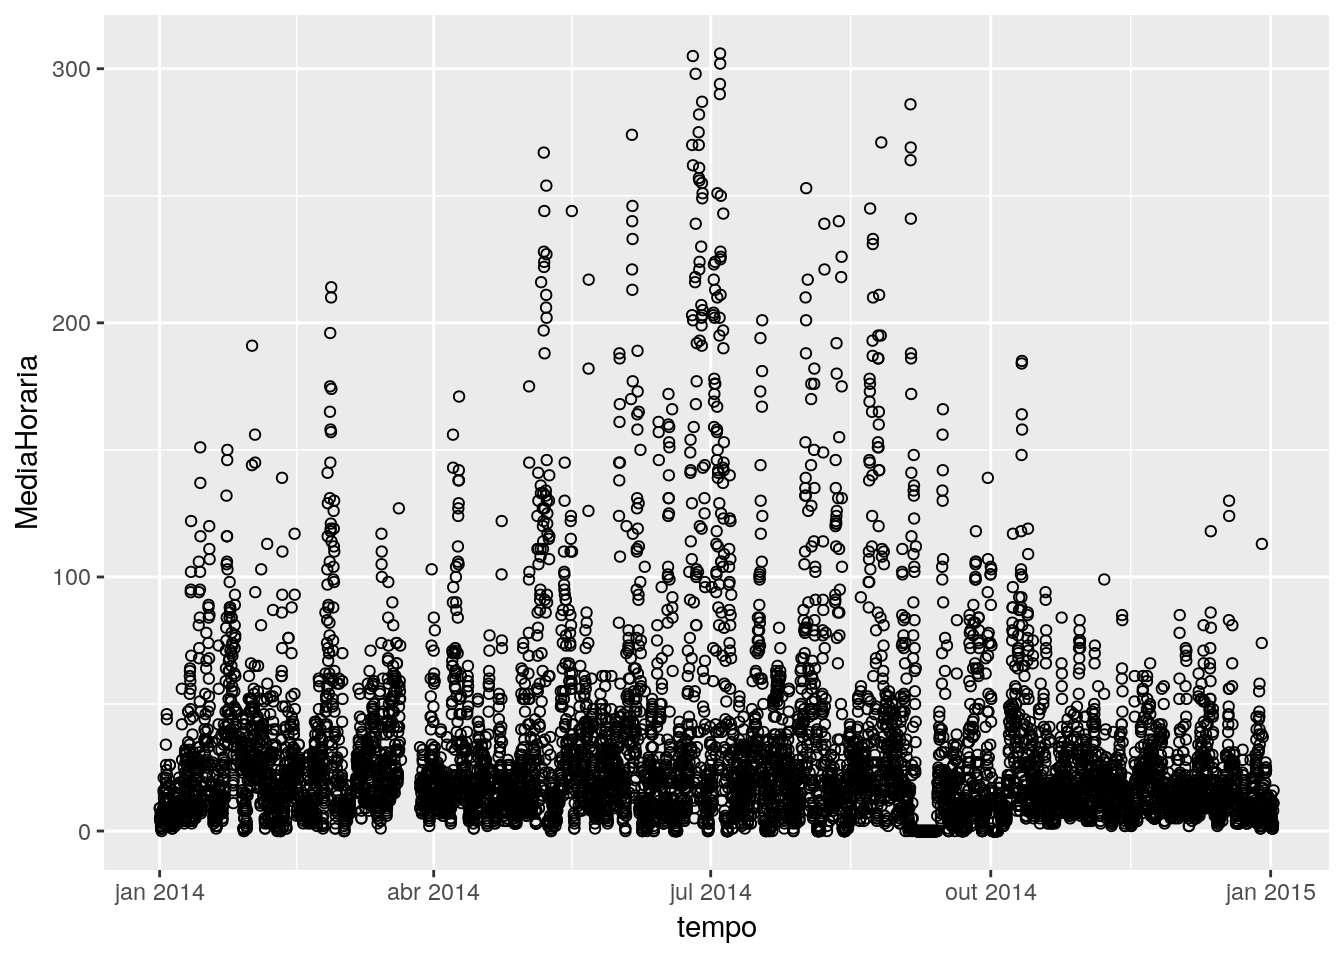
\includegraphics{cursoR_files/figure-latex/unnamed-chunk-92-1.pdf}

\begin{Shaded}
\begin{Highlighting}[]
\NormalTok{df_2014_weekly <-}\StringTok{ }\NormalTok{df_}\DecValTok{2014} \OperatorTok
\StringTok{  }\KeywordTok{group_by}\NormalTok{(Hora, weekdays) }\OperatorTok\StringTok{ }\CommentTok{#-- Agrupando os dados pelas colunas Hora e weekdays}
\StringTok{  }\KeywordTok{summarise}\NormalTok{(}\DataTypeTok{Media =} \KeywordTok{mean}\NormalTok{(MediaHoraria, }\DataTypeTok{na.rm =}\NormalTok{ T)) }\OperatorTok\StringTok{ }
\StringTok{  }\KeywordTok{ungroup}\NormalTok{() }\OperatorTok\StringTok{ }
\StringTok{  }\KeywordTok{mutate}\NormalTok{(}\DataTypeTok{Hora =} \KeywordTok{as.POSIXct}\NormalTok{(}\KeywordTok{strptime}\NormalTok{(Hora, }\StringTok{"%H:%M"}\NormalTok{))) }\OperatorTok
\StringTok{  }\KeywordTok{mutate}\NormalTok{(}\DataTypeTok{weekdays =} \KeywordTok{factor}\NormalTok{(weekdays, }\DataTypeTok{levels =} \KeywordTok{c}\NormalTok{(}\StringTok{"segunda"}\NormalTok{, }\StringTok{"terça"}\NormalTok{, }\StringTok{"quarta"}\NormalTok{,}
                                                \StringTok{"quinta"}\NormalTok{, }\StringTok{"sexta"}\NormalTok{, }\StringTok{"sábado"}\NormalTok{, }
                                                \StringTok{"domingo"}\NormalTok{))) }\CommentTok{#-- Ordenando os dias da semana}

\KeywordTok{ggplot}\NormalTok{(df_2014_weekly) }\OperatorTok{+}
\StringTok{  }\KeywordTok{scale_x_datetime}\NormalTok{(}\DataTypeTok{date_labels =} \StringTok{"%H:%M"}\NormalTok{) }\OperatorTok{+}
\StringTok{  }\KeywordTok{geom_col}\NormalTok{(}\KeywordTok{aes}\NormalTok{(}\DataTypeTok{x =}\NormalTok{ Hora, }\DataTypeTok{y =}\NormalTok{ Media), }\DataTypeTok{fill =} \StringTok{"purple"}\NormalTok{) }\OperatorTok{+}
\StringTok{  }\KeywordTok{labs}\NormalTok{(}\DataTypeTok{title =} \StringTok{"Média Horária Anual por Dia da Semana"}\NormalTok{, }\DataTypeTok{y =} \StringTok{"NOx [ppb]"}\NormalTok{) }\OperatorTok{+}
\StringTok{  }\KeywordTok{facet_wrap}\NormalTok{(}\OperatorTok{~}\StringTok{ }\NormalTok{weekdays) }\CommentTok{#-- Criando paineis em função do dia da semana}
\end{Highlighting}
\end{Shaded}

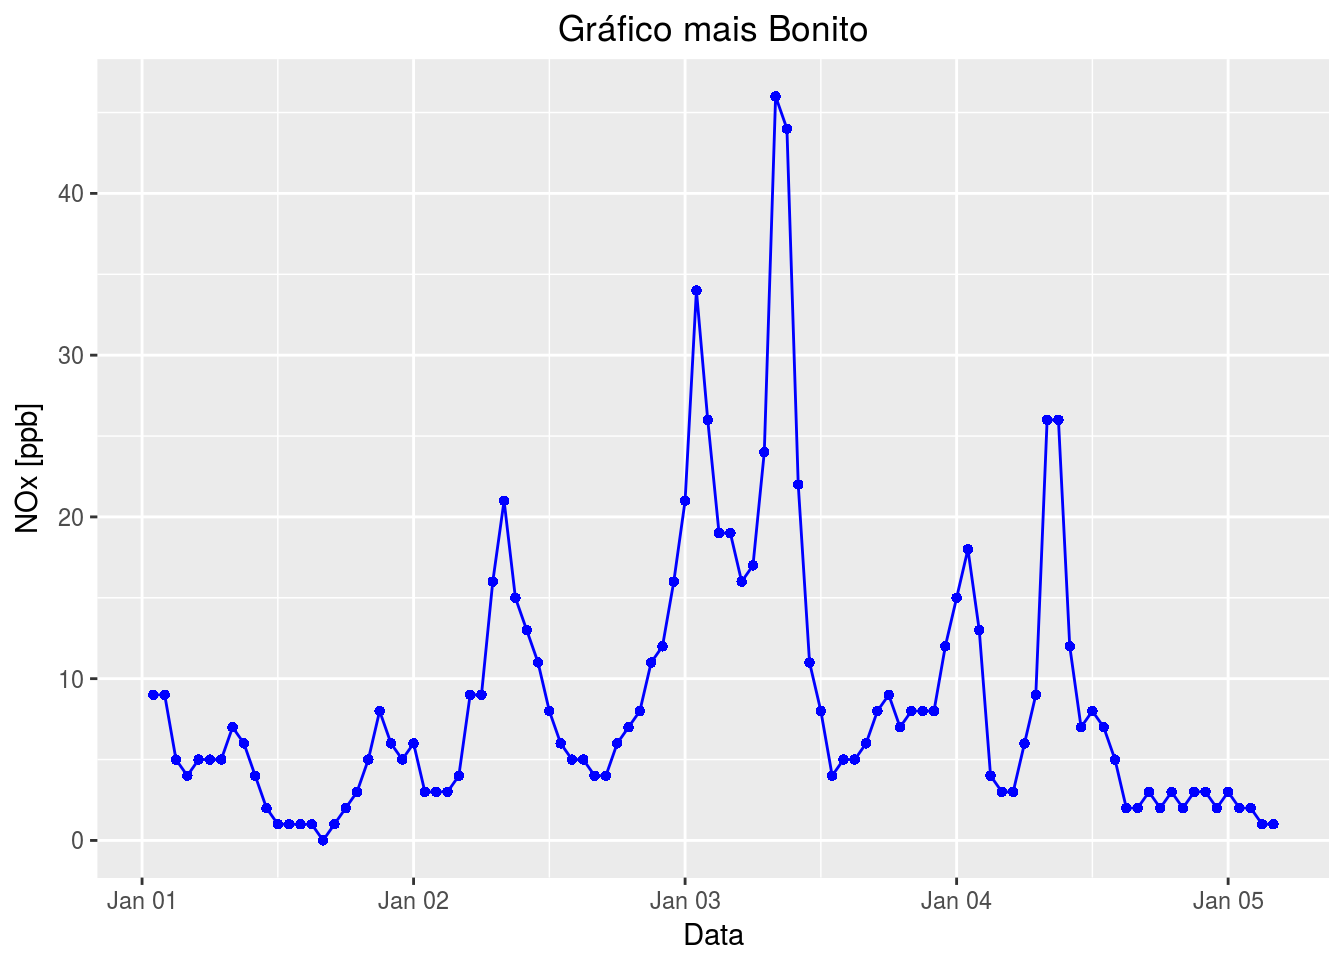
\includegraphics{cursoR_files/figure-latex/unnamed-chunk-93-1.pdf}

\begin{Shaded}
\begin{Highlighting}[]
\NormalTok{df_2014_monthly <-}\StringTok{ }\NormalTok{df_}\DecValTok{2014} \OperatorTok
\StringTok{  }\KeywordTok{group_by}\NormalTok{(Hora, mes) }\OperatorTok\StringTok{ }\CommentTok{#-- Agrupando os dados pelas colunas Hora e mes}
\StringTok{  }\KeywordTok{summarise}\NormalTok{(}\DataTypeTok{Media =} \KeywordTok{mean}\NormalTok{(MediaHoraria, }\DataTypeTok{na.rm =}\NormalTok{ T)) }\OperatorTok
\StringTok{  }\KeywordTok{ungroup}\NormalTok{() }\OperatorTok
\StringTok{  }\KeywordTok{mutate}\NormalTok{(}\DataTypeTok{Hora =} \KeywordTok{as.POSIXct}\NormalTok{(}\KeywordTok{strptime}\NormalTok{(Hora, }\StringTok{"%H:%M"}\NormalTok{))) }\OperatorTok
\StringTok{  }\KeywordTok{mutate}\NormalTok{(}\DataTypeTok{mes =} \KeywordTok{factor}\NormalTok{(mes, }\DataTypeTok{levels =} \KeywordTok{c}\NormalTok{(}\StringTok{"janeiro"}\NormalTok{, }\StringTok{"fevereiro"}\NormalTok{, }\StringTok{"março"}\NormalTok{, }
                                      \StringTok{"abril"}\NormalTok{, }\StringTok{"maio"}\NormalTok{, }\StringTok{"junho"}\NormalTok{, }\StringTok{"julho"}\NormalTok{,}
                                      \StringTok{"agosto"}\NormalTok{, }\StringTok{"setembro"}\NormalTok{, }\StringTok{"outubro"}\NormalTok{,}
                                      \StringTok{"novembro"}\NormalTok{, }\StringTok{"dezembro"}\NormalTok{))) }\CommentTok{#-- Ordenando os meses}

\KeywordTok{ggplot}\NormalTok{(df_2014_monthly) }\OperatorTok{+}
\StringTok{  }\KeywordTok{scale_x_datetime}\NormalTok{(}\DataTypeTok{date_labels =} \StringTok{"%H:%M"}\NormalTok{) }\OperatorTok{+}
\StringTok{  }\KeywordTok{geom_col}\NormalTok{(}\KeywordTok{aes}\NormalTok{(}\DataTypeTok{x =}\NormalTok{ Hora, }\DataTypeTok{y =}\NormalTok{ Media), }\DataTypeTok{fill =} \StringTok{"purple"}\NormalTok{) }\OperatorTok{+}
\StringTok{  }\KeywordTok{labs}\NormalTok{(}\DataTypeTok{title =} \StringTok{"Média Horária Anual por Mes"}\NormalTok{, }\DataTypeTok{y =} \StringTok{"NOx [ppb]"}\NormalTok{) }\OperatorTok{+}
\StringTok{  }\KeywordTok{facet_wrap}\NormalTok{(}\OperatorTok{~}\StringTok{ }\NormalTok{mes) }\CommentTok{#-- Criando paineis em função do mês}
\end{Highlighting}
\end{Shaded}

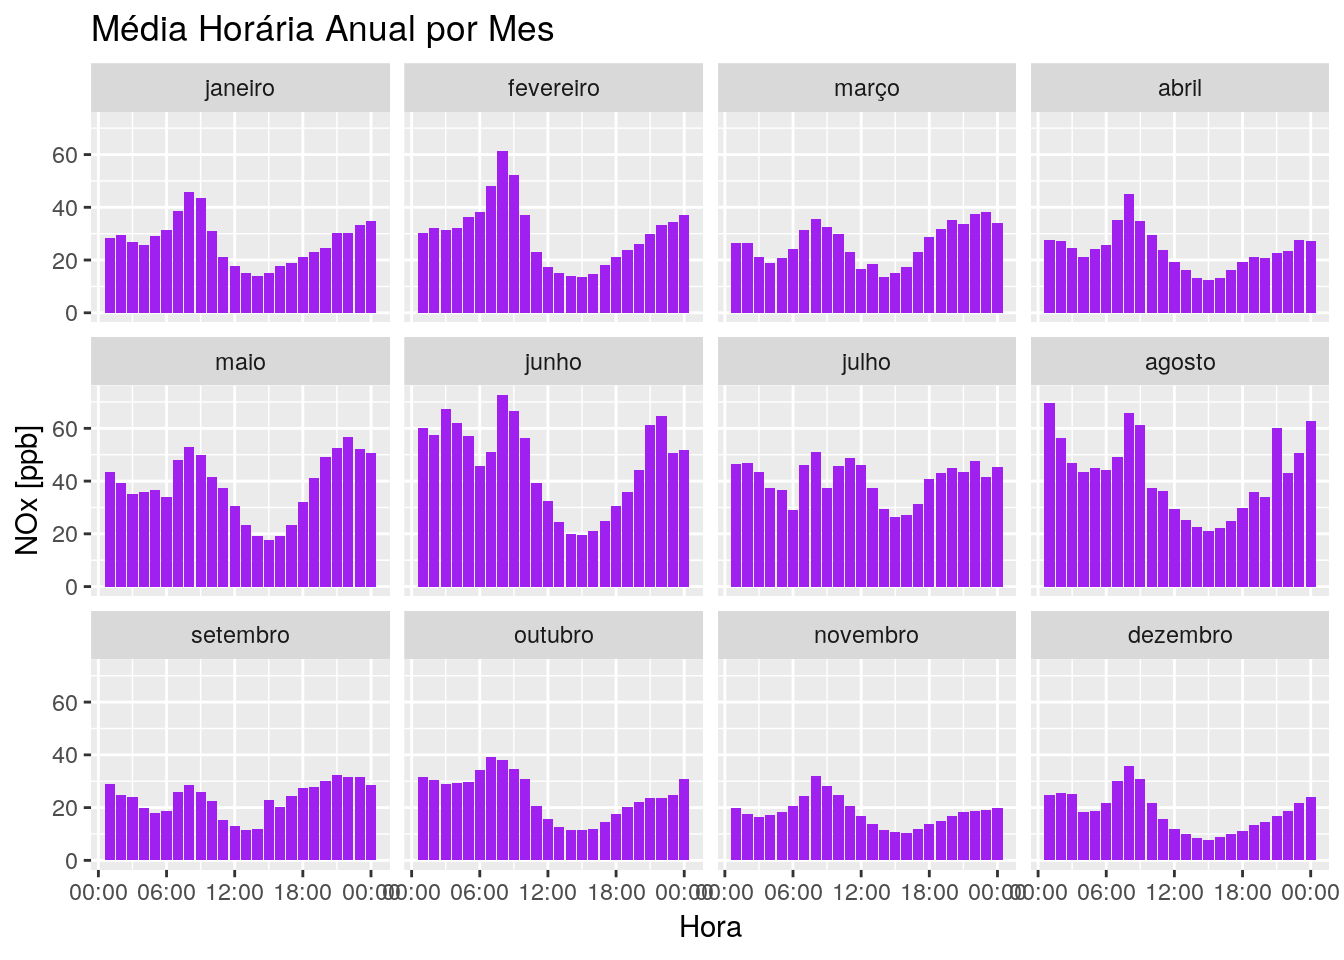
\includegraphics{cursoR_files/figure-latex/unnamed-chunk-94-1.pdf}

\begin{center}\rule{0.5\linewidth}{\linethickness}\end{center}

{\textbf{Exercício}: \emph{Em média}, como \textbf{os dados válidos} de
NOx variam mensalmente ao longo do ano de 2014? Faça um gráfico.}

{\textbf{Desafio}: Ainda é possível melhorar os gráficos acima! Pesquise
como:}

{* Diminuir a quantidade de horários no eixo x}\\
{* Separar por dias da semana e meses a partir da coluna ``tempo'', não
precisando usar as colunas de caracteres e consequentemente ordená-las
manualmente}

\begin{center}\rule{0.5\linewidth}{\linethickness}\end{center}

\subsection{Explorando outras escalas de cores e
temas}\label{explorando-outras-escalas-de-cores-e-temas}

Pacotes \textbf{veinreport} e \textbf{cptcity}

\begin{Shaded}
\begin{Highlighting}[]
\NormalTok{devtools}\OperatorTok{::}\KeywordTok{install_github}\NormalTok{(}\StringTok{"atmoschem/veinreport"}\NormalTok{)}
\end{Highlighting}
\end{Shaded}

\begin{Shaded}
\begin{Highlighting}[]
\KeywordTok{library}\NormalTok{(veinreport)}
\KeywordTok{library}\NormalTok{(cptcity)}
\end{Highlighting}
\end{Shaded}

Refazendo alguns gráficos:

\begin{Shaded}
\begin{Highlighting}[]
\KeywordTok{ggplot}\NormalTok{(df, }\KeywordTok{aes}\NormalTok{(}\DataTypeTok{x =}\NormalTok{ tempo, }\DataTypeTok{y =}\NormalTok{ MediaHoraria)) }\OperatorTok{+}\StringTok{ }
\StringTok{  }\KeywordTok{geom_line}\NormalTok{(}\KeywordTok{aes}\NormalTok{(}\DataTypeTok{color =}\NormalTok{ MediaHoraria)) }\OperatorTok{+}
\StringTok{  }\KeywordTok{labs}\NormalTok{(}\DataTypeTok{x =} \StringTok{"Data"}\NormalTok{, }\DataTypeTok{y =} \StringTok{"NOx [ppb]"}\NormalTok{) }\OperatorTok{+}
\StringTok{  }\KeywordTok{scale_color_gradientn}\NormalTok{(}\DataTypeTok{colours =} \KeywordTok{cpt}\NormalTok{()) }\OperatorTok{+}\StringTok{ }\CommentTok{#-- Definindo as cores com uma escala gradiente}
\StringTok{  }\KeywordTok{theme_black}\NormalTok{()}
\end{Highlighting}
\end{Shaded}

\begin{verbatim}
## Warning in as.POSIXlt.POSIXct(x): unknown timezone 'Americas/Sao_Paulo'
\end{verbatim}

\begin{verbatim}
## Warning in as.POSIXct.POSIXlt(from): unknown timezone 'Americas/Sao_Paulo'
\end{verbatim}

\begin{verbatim}
## Warning in as.POSIXlt.POSIXct(to): unknown timezone 'Americas/Sao_Paulo'
\end{verbatim}

\begin{verbatim}
## Warning in as.POSIXct.POSIXlt(r1): unknown timezone 'Americas/Sao_Paulo'
\end{verbatim}

\begin{verbatim}
## Warning in as.POSIXlt.POSIXct(from): unknown timezone 'Americas/Sao_Paulo'
\end{verbatim}

\begin{verbatim}
## Warning in as.POSIXct.POSIXlt(r1): unknown timezone 'Americas/Sao_Paulo'
\end{verbatim}

\begin{verbatim}
## Warning in as.POSIXlt.POSIXct(x): unknown timezone 'Americas/Sao_Paulo'
\end{verbatim}

\begin{verbatim}
## Warning in as.POSIXct.POSIXlt(from): unknown timezone 'Americas/Sao_Paulo'
\end{verbatim}

\begin{verbatim}
## Warning in as.POSIXlt.POSIXct(to): unknown timezone 'Americas/Sao_Paulo'
\end{verbatim}

\begin{verbatim}
## Warning in as.POSIXct.POSIXlt(r1): unknown timezone 'Americas/Sao_Paulo'
\end{verbatim}

\begin{verbatim}
## Warning in as.POSIXlt.POSIXct(from): unknown timezone 'Americas/Sao_Paulo'
\end{verbatim}

\begin{verbatim}
## Warning in as.POSIXct.POSIXlt(r1): unknown timezone 'Americas/Sao_Paulo'
\end{verbatim}

\begin{verbatim}
## Warning in as.POSIXlt.POSIXct(x, tz): unknown timezone 'Americas/Sao_Paulo'
\end{verbatim}

\begin{verbatim}
## Warning: Removed 1 rows containing missing values (geom_path).
\end{verbatim}

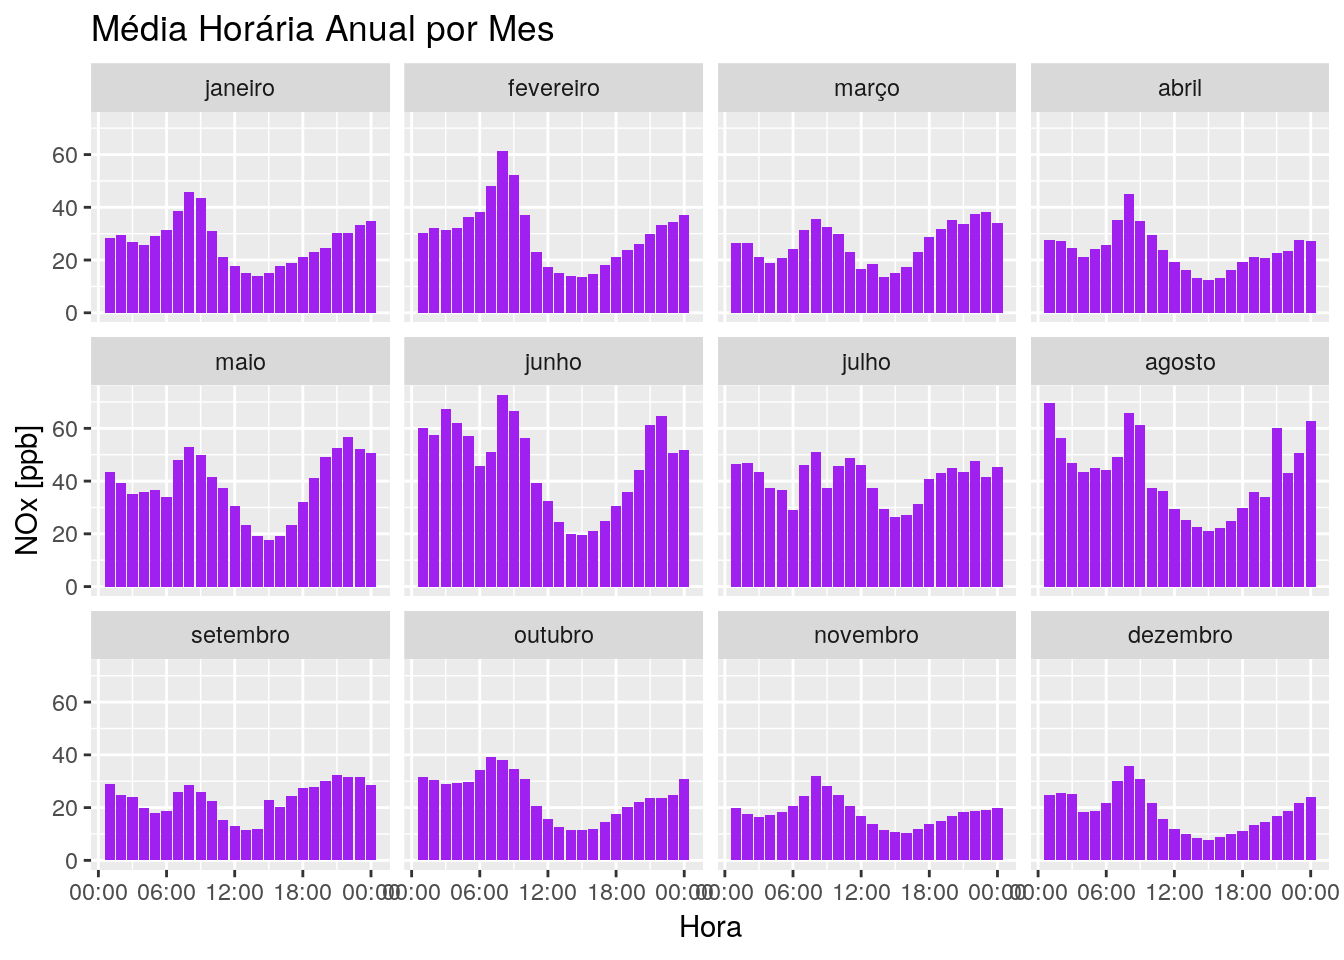
\includegraphics{cursoR_files/figure-latex/unnamed-chunk-97-1.pdf}

Experimentando escalas de cores com a função \texttt{lucky}:

\begin{Shaded}
\begin{Highlighting}[]
\KeywordTok{ggplot}\NormalTok{(df_2014_monthly) }\OperatorTok{+}
\StringTok{  }\KeywordTok{scale_x_datetime}\NormalTok{(}\DataTypeTok{date_labels =} \StringTok{"%H:%M"}\NormalTok{) }\OperatorTok{+}
\StringTok{  }\KeywordTok{geom_col}\NormalTok{(}\KeywordTok{aes}\NormalTok{(}\DataTypeTok{x =}\NormalTok{ Hora, }\DataTypeTok{y =}\NormalTok{ Media, }\DataTypeTok{fill =}\NormalTok{ Media)) }\OperatorTok{+}
\StringTok{  }\KeywordTok{labs}\NormalTok{(}\DataTypeTok{title =} \StringTok{"Média Horária Anual por Mes"}\NormalTok{, }\DataTypeTok{y =} \StringTok{"NOx [ppb]"}\NormalTok{) }\OperatorTok{+}
\StringTok{  }\KeywordTok{scale_fill_gradientn}\NormalTok{(}\DataTypeTok{colors =} \KeywordTok{lucky}\NormalTok{()) }\OperatorTok{+}\StringTok{ }\CommentTok{#-- Definindo as cores com uma escala gradiente aleatória}
\StringTok{  }\KeywordTok{theme_black}\NormalTok{() }\OperatorTok{+}
\StringTok{  }\KeywordTok{theme}\NormalTok{(}\DataTypeTok{legend.position =} \StringTok{"bottom"}\NormalTok{, }\DataTypeTok{legend.direction =} \StringTok{"horizontal"}\NormalTok{) }\OperatorTok{+}\StringTok{ }\CommentTok{#-- Colocando a legenda na parte de baixo da figura}
\StringTok{  }\KeywordTok{facet_wrap}\NormalTok{(}\OperatorTok{~}\StringTok{ }\NormalTok{mes) }\CommentTok{#-- Criando paineis em função do mês}
\end{Highlighting}
\end{Shaded}

\begin{verbatim}
## Colour gradient: go2_webtwo_grey_g0_2, number: 3263
\end{verbatim}

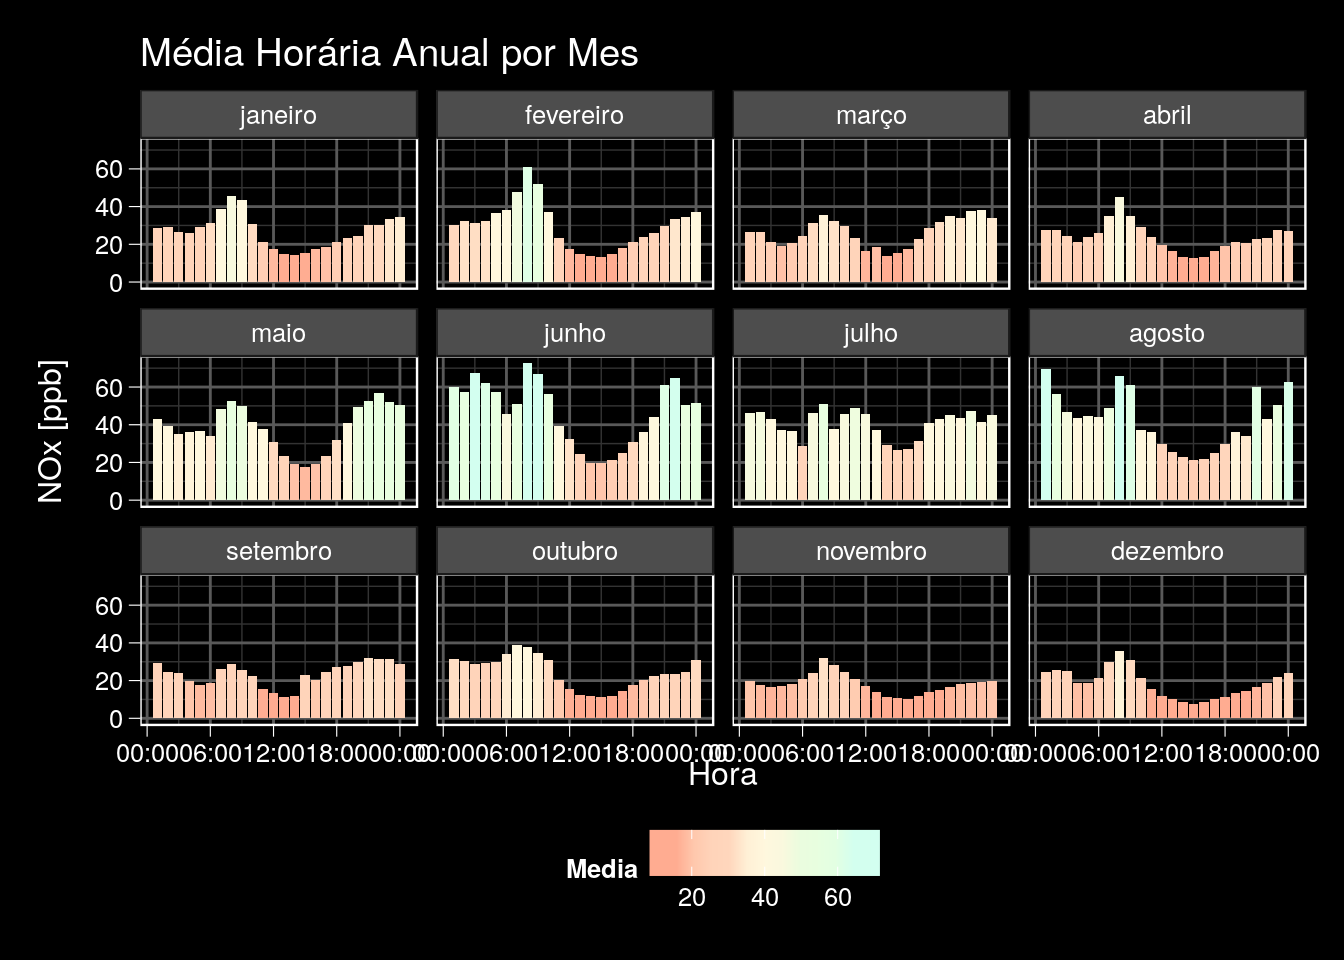
\includegraphics{cursoR_files/figure-latex/unnamed-chunk-98-1.pdf}

\textbf{Este é só o começo!}
\href{http://r-statistics.co/Top50-Ggplot2-Visualizations-MasterList-R-Code.html}{Veja
aqui um pouco mais das muitas aplicações do \texttt{ggplot}}.

\chapter{Estruturas de Controle}\label{loop}

Em breve.

\section{if-else}\label{if-else}

\section{for}\label{for}

\section{while}\label{while}

\section{repeat}\label{repeat}

\section{lapply}\label{lapply}

\section{sapply}\label{sapply}

\section{split}\label{split}

\section{tapply}\label{tapply}

\section{apply}\label{apply}

\section{mapply}\label{mapply}

\chapter{De Scripts a Funções e de Funções a Pacotes}\label{fx}

Em breve.

\chapter{\texorpdfstring{Geo Spatial: \texttt{raster}, \texttt{sf} e
\texttt{stars}}{Geo Spatial: raster, sf e stars}}\label{geo}

Em breve.

\begin{itemize}
\tightlist
\item
  \href{https://leanpub.com/rprogramming}{R Programming for Data Science
  (Leanpub)}\\
\item
  \href{http://www.cookbook-r.com/Graphs/}{R Graphics Cookbook (Cookbook
  for R)}\\
\item
  \href{https://cran.r-project.org/doc/manuals/r-release/R-intro.html}{An
  Introduction to R (CRAN)}\\
\item
  \href{https://cran.r-project.org/doc/manuals/r-release/R-data.html}{R
  Data Import/Export (CRAN)}\\
\item
  \href{https://www.rstudio.com/resources/cheatsheets/}{RStudio Cheat
  Sheets (RStudio)}\\
\item
  \href{https://www.rstudio.com/resources/webinars/}{Webinars and Videos
  On Demand (RStudio)}\\
\item
  \href{https://www.rstudio.com/online-learning/}{Online Learning
  (RStudio)}\\
\item
  \href{https://www.tidyverse.org/learn/}{Learn the tidyverse
  (Tidyverse)}
\item
  \href{https://cran.r-project.org/doc/manuals/r-release/R-exts.html}{Writing
  R Extensions (CRAN)}\\
\item
  \href{https://cran.r-project.org/doc/manuals/r-release/R-ints.html}{R
  Internals (CRAN)}\\
\item
  \href{https://cran.r-project.org/doc/manuals/r-release/R-lang.html}{R
  Language Definition (CRAN)}
\end{itemize}

\begin{center}\rule{0.5\linewidth}{\linethickness}\end{center}

\emph{Quer fazer um documento com o mesmo estilo do nosso? Leia}
\href{https://bookdown.org/yihui/bookdown/}{bookdown: Authoring Books
and Technical Documents with R Markdown (bookdown.org)}

\bibliography{book.bib,packages.bib}


\end{document}
